% !Mode:: "TeX:UTF-8"
%!TEX program = xelatex
%\expandafter\def\csname CTEX@spaceChar\endcsname{\hspace{1em}}
\documentclass[single,print]{sduthesis}
% !Mode:: "TeX:UTF-8"
% titlepageinfo.tex
% 中图分类号
\fenlei{TP391}
% 单位代号
\DWdaihao{10422}
% 密级
\miji{公开}
% 学号
\StuNum{1901-2012}
% 页眉
\ThesisHeader{山东大学硕士学位论文}
\EThesisHeader{Shandong University Master Thesis}
% 论文类型(封面) 中
\CThesisType{硕~士~学~位~论~文}
% 论文类型(封面) 英
\EThesisType{Thesis for Master Degree}
% 中文标题
\Ctitle{山东大学研究生学位论文\LaTeX{}模板}
% 英文标题
\Etitle{SDU Thesis Template For Postgraduate}
% 作者中文名
\Cauthor{德尔伯特}
% 学院
\Dpart{某某学院}
% 专业中文名
\Cmajor{某某专业}
% 年级
\Grade{2012级}
% 指导老师中文名
\Csuperver{某某~~教授}
\Ccosuperver{某某~~教授}
% 中文日期
\Cdate{\today}
\title{\the\Ctitle}
\author{\the\Cauthor}
\date{\the\Cdate}
% !Mode:: "TeX:UTF-8"
% usersettings.tex
\usepackage{paralist}
\usepackage{dtklogos}
\usepackage{xcolor}
\usepackage{listings}
\usepackage{tabularx}
\usepackage{setspace}
\usepackage{mathptmx} 

\usepackage{fontspec}
\setmainfont{Times New Roman}

%\usepackage{mathspec}
%\setallmathfont{Times New Roman}
\usepackage{array}%表格线条
% Add Chapter to TOC && Remove Contents from TOC
\usepackage[chapter, nottoc]{tocbibind}
% 允许使用子图 subfloat
\usepackage{subfig}
% 允许使用图文混排
\usepackage{wrapfig}
% picinpar 和 picins 都无法成功实现图文混排。
% \usepackage{picinpar}
% \usepackage{picins}
% 使用 ccmap,则英文和数字都正常。如果论文重复率高的话,注释掉 ccmap ,英文和数字被映射为汉字,相当于增加干扰码,降低重复率。
\usepackage{ccmap}
%\usepackage{calc}
%\usepackage{times}%%新加Times New Roman
\usepackage{ragged2e}
\usepackage{titlesec}
%\usepackage{algorithmic}
%\usepackage{algorithm}
%\usepackage[ruled,linesnumbered]{algorithm2e}
\usepackage{enumitem}
\usepackage{diagbox}

\allowdisplaybreaks[4]
% \newtheorem{环境名}[编号延续]{显示名}[编号层次]
% 在下例中,我们定义了四个环境:定义、定理、引理和推论,它们都在一个section内编号,而引理和推论会延续定理的编号。
\newtheorem{definition}{定义}[section]
\newtheorem{theorem}{定理}[section]
\newtheorem{lemma}[theorem]{引理}
\newtheorem{corollary}[theorem]{推论}
\renewcommand{\proofname}{证明}
\newtheorem{remark}{注}[section]

\definecolor{SDUred}{RGB}{135,45,36}
\lstset{language=TeX}
% \lstset{extendedchars=false}
\lstset{breaklines}	
\lstset{numbers=left,numberstyle=\tiny,%commentstyle=\color{red!50!green!50!blue!50},
frame=shadowbox,rulesepcolor=\color{red!20!green!20!blue!20},escapeinside=``,
xleftmargin=2em,xrightmargin=2em,aboveskip=1em,backgroundcolor=\color{red!3!green!3!blue!3},
basicstyle=\small\ttfamily,stringstyle=\color{purple},keywordstyle=\color{blue!80}\bfseries,
commentstyle=\color{olive}}
\numberwithin{footnote}{page}
\renewcommand{\thefootnote}{\arabic{footnote}}
\renewcommand{\CTeX}{\SHUANG{C}\TeX}


\begin{document}

% 首页及原创性声明
\maketitlepagestatement
\cleardoublepage
% 大写罗马页码
\pagenumbering{Roman}\setcounter{page}{1}

\cleardoublepage
% 中英文摘要
% !Mode:: "TeX:UTF-8"
\begin{cnabstract}

\verb|SDUthesis Template for Postgraduate|是符合山东大学研究生毕业论文格式要求的\LaTeX{}格式的模板。

\textbf{本示例文档提供了章}节、图像、表格、引用等的编写方法示例。

\cnkeywords{论文;模板;\LaTeX{}}

\end{cnabstract}

\begin{enabstract}

This is an English Abstract.

\enkeywords{English; Abstract}

\end{enabstract}

% Chinese TOC
%\pagenumbering{Roman}\setcounter{page}{1}
% \begin{KeepFromToc}
\maketableofcontents
%\end{KeepFromToc}
%\cleardoublepage
% English TOC
\tableofengcontents
\begin{symboldescription}


%	\begin{table}[h]
%		\centering
		\begin{tabularx}{\textwidth}{X X }
			 
			 $\mathbb{C}$ & 复平面 \\
			 $\mathbb{R}$ & 实数轴 \\
			 $\lambda_{1}$ & 最小特征值 \\
			 $\lambda_{N}$ & 最大特征值 \\
			 $\mathcal{E}_h$ & 离散误差 \\
			 $\mathcal{E}_R$ & 右截断误差 \\
			 $\mathcal{E}_L$ & 左截断误差 \\
			 $\mathcal{E}_Q$ & 近似误差 \\
		\end{tabularx}
%	\end{table}
\end{symboldescription}




\newpage


% 阿拉伯数字页码
\pagenumbering{arabic}\setcounter{page}{1}

% 正文
\setlength\baselineskip{20pt}\selectfont
% \input{contents/body.tex}
% !Mode:: "TeX:UTF-8"
\chapter{绪论}
\echapter{Introduction}

\section{中英文标题如何自动生成到目录当中}
\esection{How the TOC filled with Chinese and English Titles}

中英文标题如何自动生成到目录当中请自行对照各个章节源码。

本示例文档所用填充文字来自 Google 条款: \url{https://www.google.com.hk/intl/zh-CN/policies/terms/regional.html} 。
% !Mode:: "TeX:UTF-8"
\chapter{正文编写}
\echapter{How to write}

本章节介绍了如何插入公式、图片、表格、引用等。

\section{插入图片}
\esection{How to Insert a Figure}

\begin{figure}[htbp]
\centering
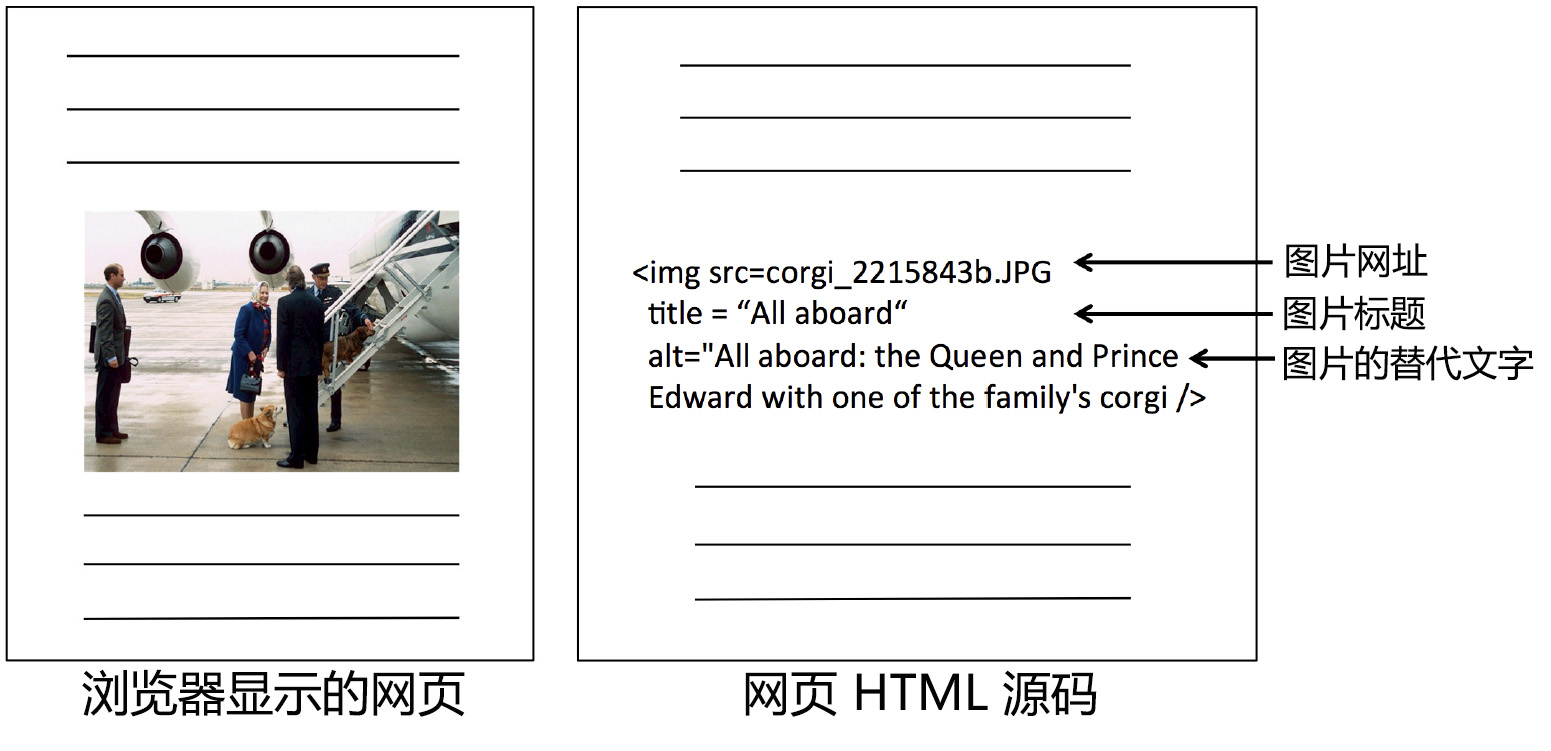
\includegraphics[width=0.8\textwidth]{htmltext.jpg}
\caption{图片在网页中的显示}
\label{FIGhtmltext}
\end{figure}

使用\verb|figure|标记,设置宽度、图片文件名、标题、标签。

插入子图片:

\begin{figure}[htbp]
\centering
\subfloat[GIST]{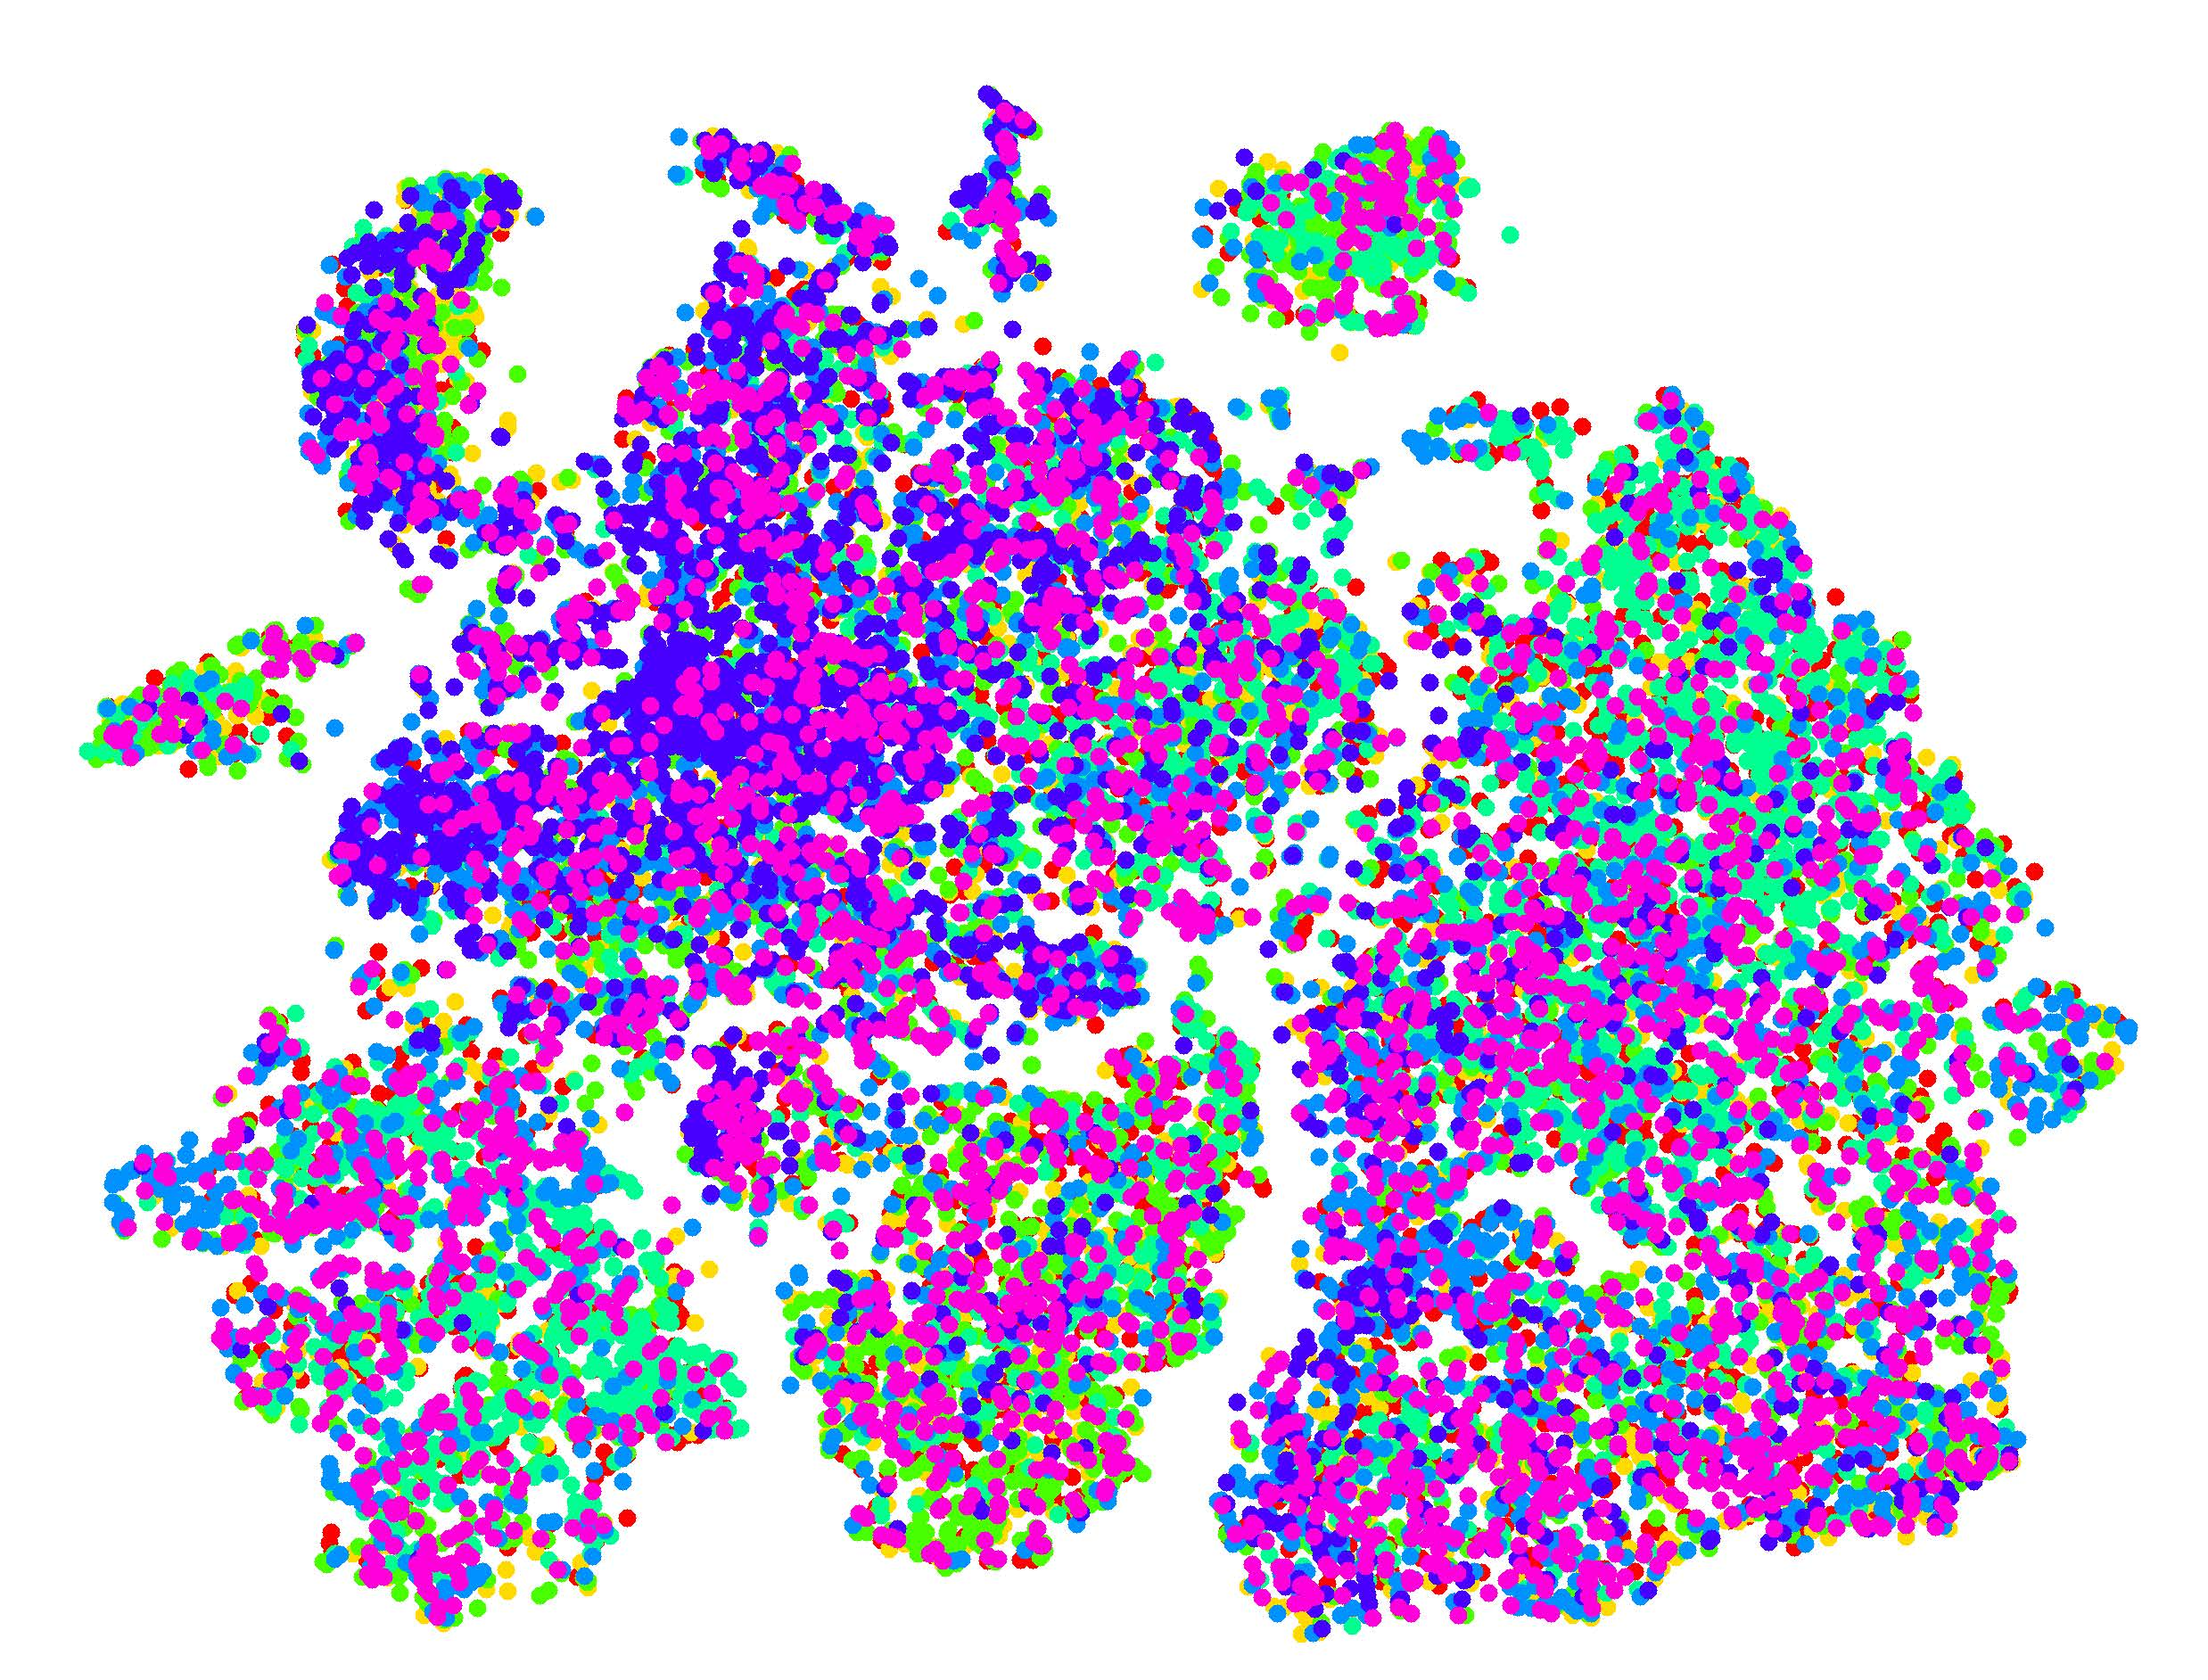
\includegraphics[width=0.3\textwidth]{GIST.jpg}}
~~
\subfloat[DeCAF$_1$]{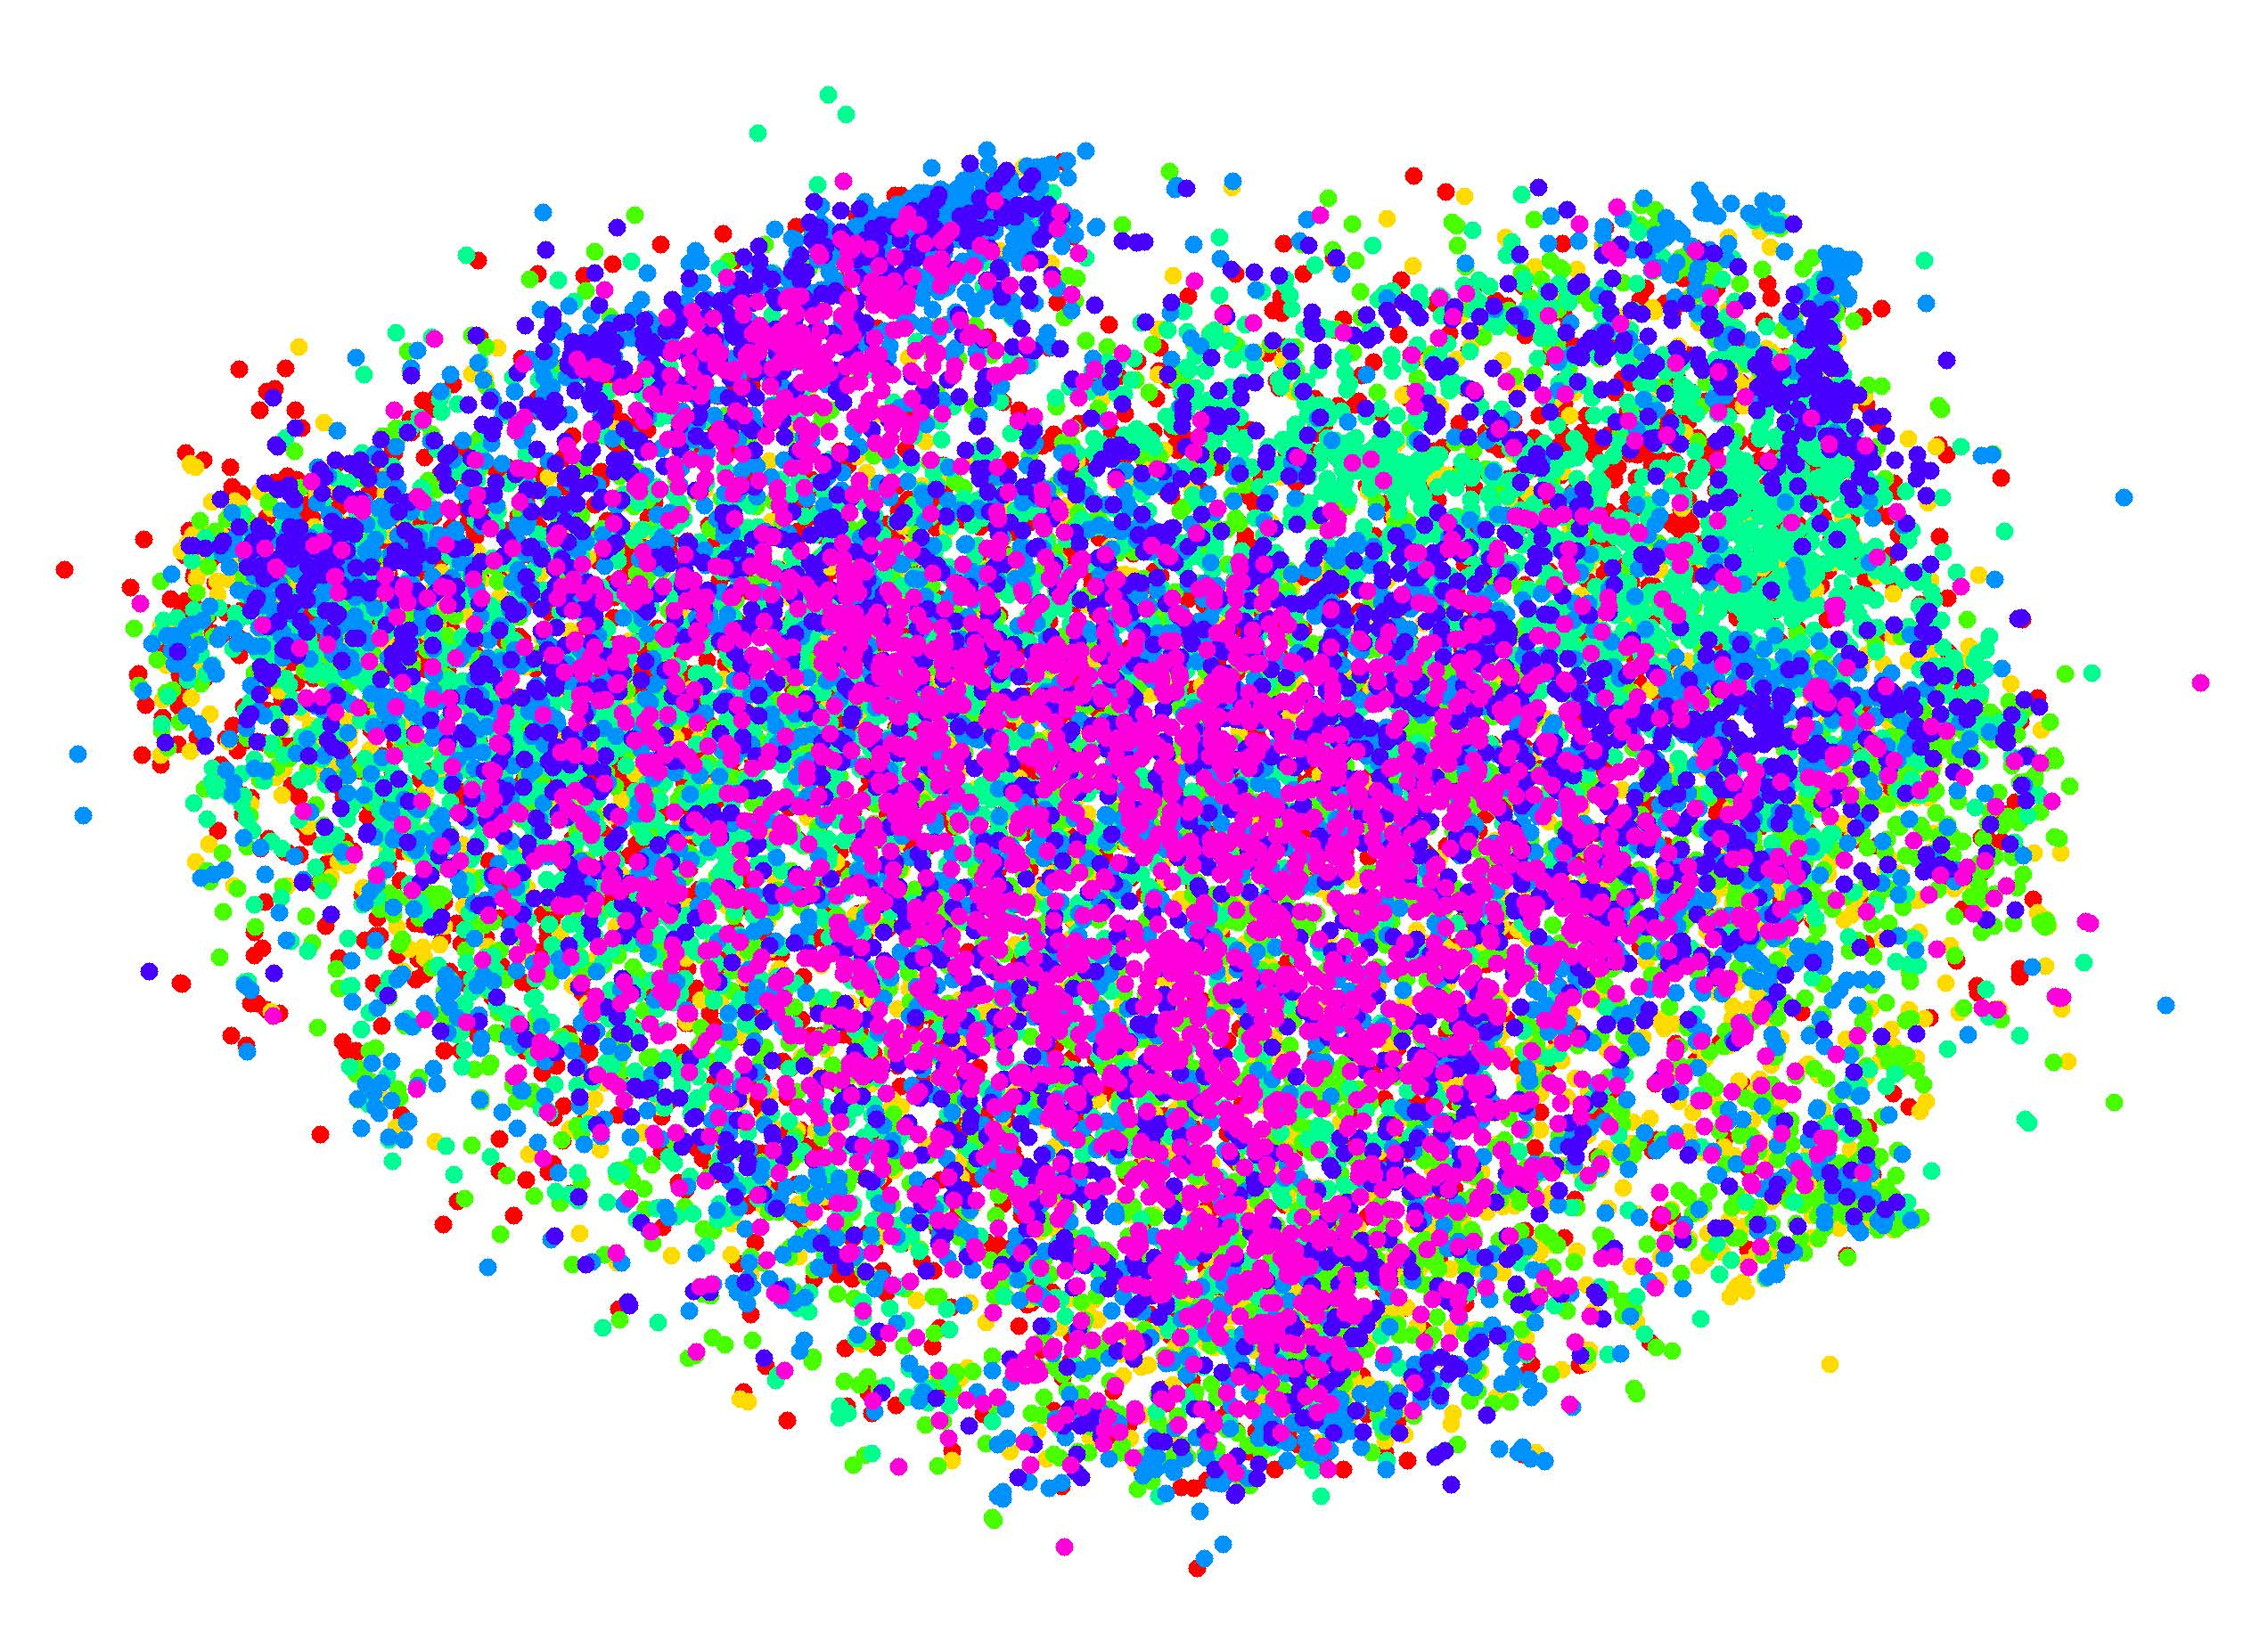
\includegraphics[width=0.3\textwidth]{DECAF1.jpg}}
~~
\subfloat[DeCAF$_6$]{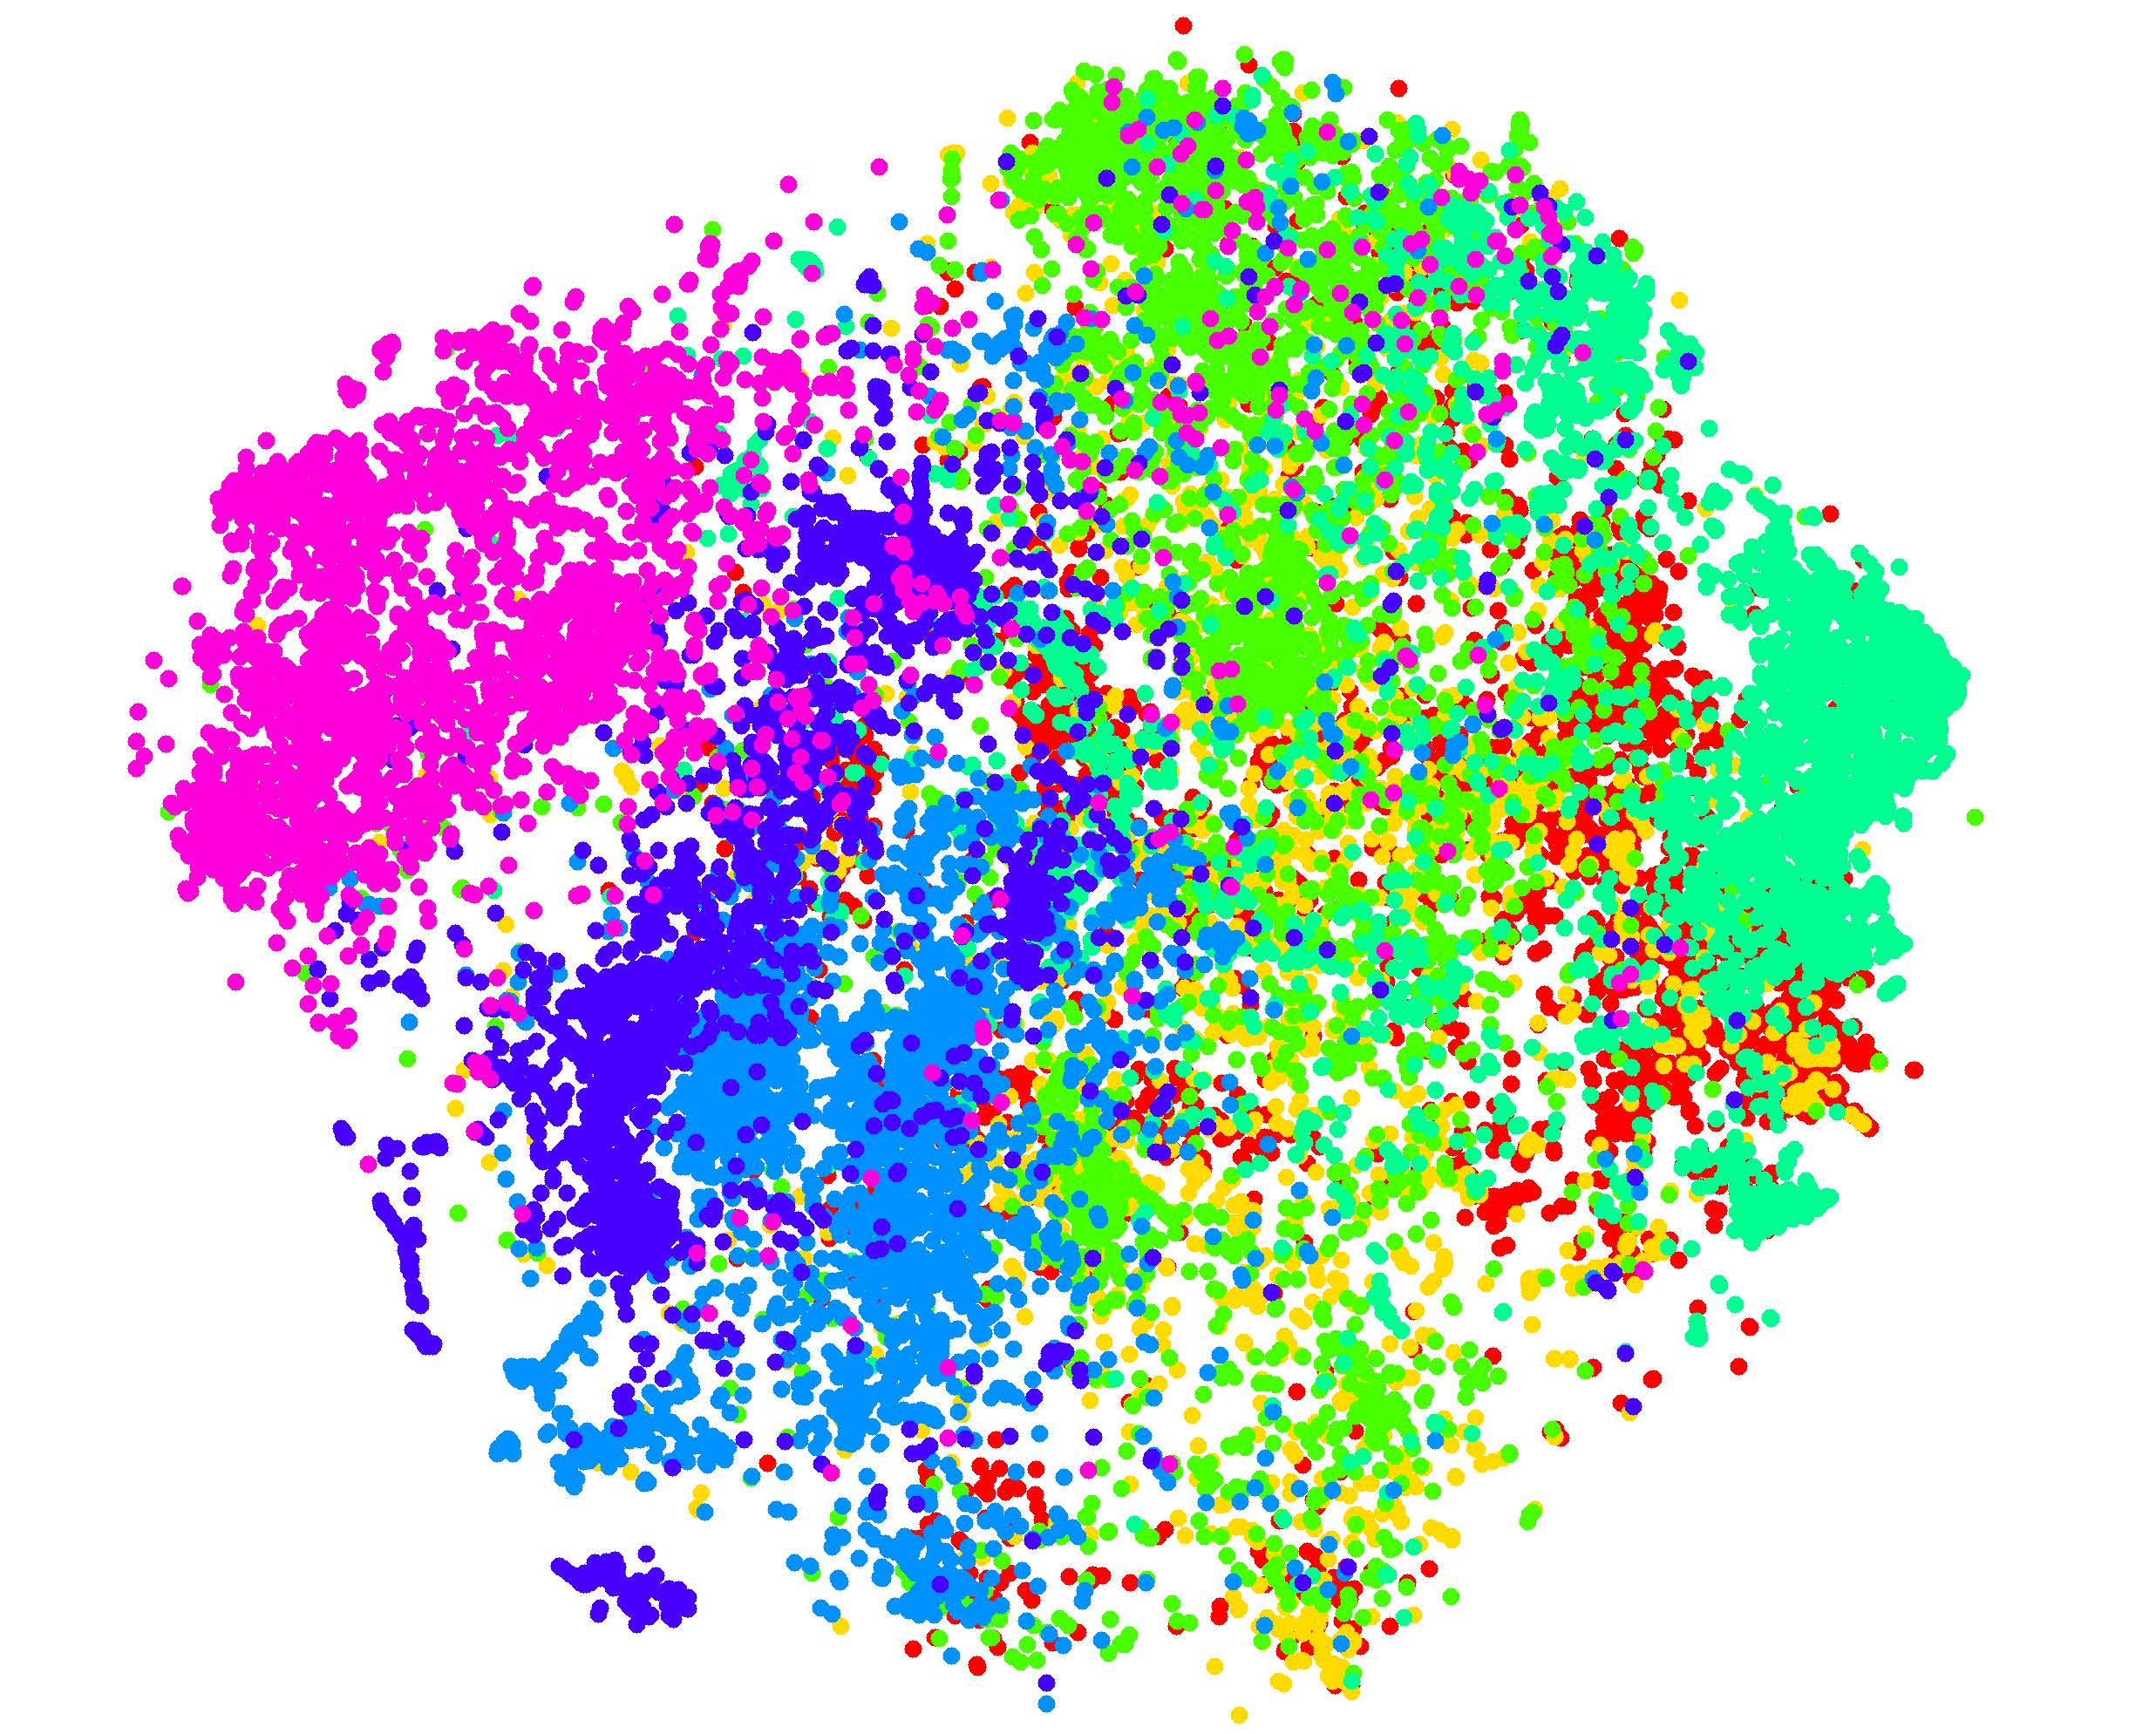
\includegraphics[width=0.3\textwidth]{DECAF6.jpg}}
\caption{这是标题}
\label{thisiisalabel}
\end{figure}

使用服务

您必须遵守服务中提供的所有政策。

请勿滥用我们的服务。举例而言,请勿干扰我们的服务或尝试使用除我们提供的界面和指示以外的方法访问这些服务。您仅能在法律(包括适用的出口和再出口管制法律和法规)允许的范围内使用我们的服务。如果您不遵守我们的条款或政策,或者我们在调查可疑的不当行为,我们可以暂停或停止向您提供服务。

\section{插入章节}
\esection{Insert Sections}

\subsection{二级章节}
\esubsection{Subsection}

使用我们的服务并不让您拥有我们的服务或您所访问的内容的任何知识产权。除非您获得相关内容所有者的许可或通过其他方式获得法律的许可,否则您不得使用服务中的任何内容。本条款并未授予您使用我们服务中所用的任何商标或标志的权利。请勿删除、隐藏或更改我们服务上显示的或随服务一同显示的任何法律声明。

我们的服务会显示一些不属于 Google 的内容。这些内容由发布的实体承担全部责任。我们可能会审查相关内容,以确定其是否违法或违反了我们的政策;如果我们有理由相信该内容违反了我们的政策或违法,我们可以将其删除或拒绝显示。不过,这并不意味我们必然会审查内容,因此请勿想当然地认为我们在进行审查。

在您使用服务的过程中,我们可能会向您发送服务公告、管理消息和其他信息。您可以选择不接收上述某些信息。

我们的部分服务可在移动设备上使用。在使用此类服务时,请勿因此而分散注意力和违反交通或安全法。

\section{插入表格}
\esection{Insert Tables}

\begin{table}[htbp]
\centering
\caption{表格示例}\label{TABfeatures}
\begin{tabular}
{ccccccc}
\toprule
Colorhist& GETLF& GIST& SIFT& C-SIFT& RGB-SIFT& OPPONENT-SIFT\\
\hline
576& 256& 480& 5000& 5000& 5000& 5000\\
\bottomrule
\end{tabular}
\end{table}

为了使用我们的某些服务,您可能需要一个 Google 帐户。您可以创建自己的 Google 帐户或者由管理员(例如您所在的单位或教育机构)为您分配 Google 帐户。如果您使用的是由管理员分配的 Google 帐户,可能需要遵守另外的条款或附加条款,并且您的管理员可能有权访问或停用您的帐户。

为保护您的 Google 帐户,请务必保管好您的密码并对外保密。您应对自己 Google 帐户上发生的活动或通过该帐户进行的活动负责。尽量不要在第三方应用中使用与 Google 帐户相同的密码。如果您发现有人在未经授权的情况下使用了您的密码或 Google 帐户,请按这些指示操作。

\section{插入公式}
\esection{How to Insert an Equation}

\begin{equation}\label{EQKeywordWeight}
s(t_n) = \frac{1}{\sum_{\forall t\in\tau}s(t)} \sum_{\forall t_{n,m}\in\tau}F_{n,m}\mathrm{sigm}(\mathrm{d}_{n,m})
\end{equation}

\section{插入列表}
\esection{How to Insert an List}

我们会根据美国《数字千年版权法》规定的流程,对涉嫌侵犯版权的通知作出回应并终止屡次侵权人的帐户。

我们会向版权持有人提供信息,以帮助他们在线管理自己的知识产权。如果您认为有人侵犯了您的版权并希望通知我们,可以在我们的帮助中心内查阅有关提交通知的信息和 Google 关于回应通知的政策。

\begin{enumerate}

\item 条目 1。
\item 条目 2(第 $n_l$ 层),计算:

        $$
        \delta^{(n_l)} = - (y - a^{(n_l)}) \bullet f'(z^{(n_l)})
        $$ 

\item 对于 $l = n_l-1, n_l-2, n_l-3, \ldots, 2$ 的各层。
\item 条目 4。

        \[ 
        \begin{aligned}
        \nabla_{W^{(l)}} J(W,b;x,y) &= \delta^{(l+1)} (a^{(l)})^T, \\
        \nabla_{b^{(l)}} J(W,b;x,y) &= \delta^{(l+1)} 
        \end{aligned}
        \]
\end{enumerate}

隐私与版权保护

Google 的隐私权政策介绍了您在使用我们的服务时,我们会如何处理您的个人数据和保护您的隐私。使用我们的服务即表示您同意 Google 可以按照我们的隐私权政策使用您的个人数据。

我们会根据美国《数字千年版权法》规定的流程,对涉嫌侵犯版权的通知作出回应并终止屡次侵权人的帐户。

我们会向版权持有人提供信息,以帮助他们在线管理自己的知识产权。如果您认为有人侵犯了您的版权并希望通知我们,可以在我们的帮助中心内查阅有关提交通知的信息和 Google 关于回应通知的政策。

\section{图片表格混合插入}
\esection{Mix with Images and Tables}

文字多时,使用\verb|\tabincell|进行插入。注意需要使用手动\\
换行。

\begin{table}[htbp]
\centering
\caption{图片表格混合插入}\label{TABBP1resultdemo}
\begin{tabular}
{cll}
\toprule
类别      &示例图片1  &示例图片2  \\
\hline
图像&
\tabincell{c}{
\includegraphics[width=0.35\textwidth]{9ddQpU7yeNmEzUXu.jpg}\\9ddQpU7yeNmEzUXu.jpg} &
\tabincell{c}{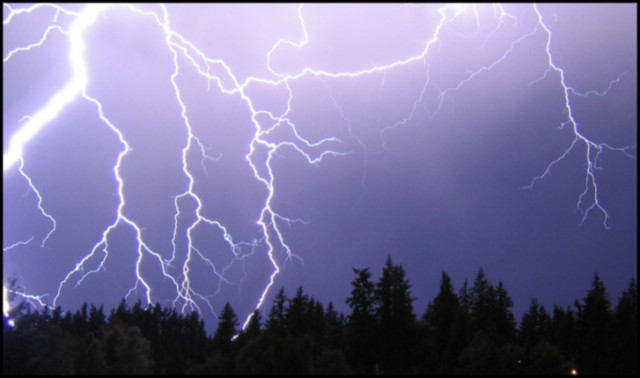
\includegraphics[width=0.42\textwidth]{9_cX52_TUIjODdac.jpg}\\9\_cX52\_TUIjODdac.jpg} \\

\hline

\tabincell{c}{Ground\\Truth} &
\tabincell{l}{keywords keywords\\
keywords keywords} &
\tabincell{l}{keywords 垂直居中} \\

\bottomrule
\end{tabular}
\end{table}

\section{插入引用}
\esection{How to Insert a Citation}

引用公式\ref{EQKeywordWeight}。

引用图片\ref{thisiisalabel}。

引用表格\ref{TABfeatures}。

引用参考文献\cite{smeulders2000content}。

% % !Mode:: "TeX:UTF-8"
\chapter{${A}^{-\alpha}$的近似}
\echapter{Approximation of ${A}^{-\alpha}$}

To begin, let's focus on the numerical solution of the following equation:
\begin{equation}
	(-\Delta)^\alpha u = f 
\end{equation}

We can get
\begin{equation}
	u = (-\Delta)^{-\alpha} f
\end{equation}

The primary challenge lies in approximating the operator $A^{-\alpha}$, where $A$ denotes the discretized matrix representation of the Laplace operator.

Using the Cauchy integral formula:
\begin{equation}
	f(A)=\frac{1}{2 \pi i} \int_T f(s)(s-A)^{-1} d s
\end{equation}

Letting $f(A) = A^{-\alpha}$, we have:
\begin{equation}
	A^{-\alpha}=\frac{1}{2 \pi i} \int_T s^{-\alpha}(s-A)^{-1} d s
\end{equation}

Since there are no singularities on the negative real axis, We can split the contour along the negative real axis:
\begin{equation}
	\begin{aligned}
	A^{-\alpha}&=\frac{1}{2 \pi i} \int_{-\infty}^0(s+i 0)^{-\alpha}(s-A)^{-1} d s+\frac{1}{2 \pi i} \int_0^{-\infty}(s-i 0)^{-\alpha}(s-A)^{-1} d s \\
	&=\frac{1}{2 \pi i} \int_{-\infty}^0[(s+i 0)^{-\alpha}-(s-i 0)^{-\alpha}](s-A)^{-1} d s\\
	&=-\frac{1}{2 \pi i} \int_{0}^{+\infty}[(-s+i 0)^{-\alpha}-(-s-i 0)^{-\alpha}](s+A)^{-1} d s\\
	&=-\frac{1}{2 \pi i} \int_{0}^{+\infty}[(se^{i \pi})^{-\alpha}-(se^{-i \pi})^{-\alpha}](s+A)^{-1} d s\\
	&=-\frac{1}{2 \pi i} \int_{0}^{+\infty}[s^{-\alpha}(e^{-i \pi\alpha}-e^{i \pi \alpha})](s+A)^{-1} d s\\
\end{aligned}
\end{equation}

We can simplify the term $e^{-i\pi\alpha}-e^{i\pi\alpha}$ as follows:
\begin{equation}
	\begin{aligned}
	&e^{-i \pi\alpha}-e^{i \pi \alpha}\\
	=&[\cos(\pi \alpha)-i \sin(\pi \alpha)]-[\cos(\pi \alpha)+i \sin(\pi \alpha)]\\
	=&-2 i \sin(\pi \alpha)
\end{aligned}
\end{equation}

Hence, $A^{-\alpha}$ can be transformed to the $Balakrishnan$  integral \cite{Balakrishnan1960FractionalPO} when $\alpha \in(0,1)$:
\begin{equation}
	\begin{aligned}
	A^{-\alpha}& =-\frac{1}{2 \pi i} \int_{0}^{+\infty}[s^{-\alpha}(2 i \sin(\pi\alpha))](s+A)^{-1} d s\\
	& =\frac{\sin(\pi \alpha)}{\pi} \int_{0}^{+\infty} s^{-\alpha}(s+A)^{-1} d s
\label{original}
\end{aligned}
\end{equation}

We want to seek a suitable summation formula to approximate the  $Balakrishnan$  integral for constant fractional order $\alpha$ ,i.e.,
\begin{equation}
{A}^{-\alpha}=\sum_{j=0}^{Q}w_j(\lambda_jI+A)^{-1}
\end{equation}


\section{基于Single-Exponential (SE)的$A^{-\alpha}$近似}
\esection{Single-Exponential (SE) formulas }


By using  $s=e^{\mu x}$ in $\eqref{original}$\cite{Harizanov2020ASO} , we can get $s'(x)=\mu e^{\mu x}$ and
\begin{equation}
{A}^{-\alpha}=\frac{\sin(\pi \alpha)}{\pi}\int_{-\infty}^{+\infty}e^{-\alpha\mu x}(e^{\mu x} I+A)^{-1}\mu e^{\mu x} dx
\label{expu}
\end{equation}

Define the integrand
\begin{equation}
f(x)=\frac{\mu e^{(1-\alpha)\mu x}}{e^{\mu x}+A}
\label{function_SE}
\end{equation}

For different $\alpha$ and $A$, $\mu=1$, we plot the integrand f(x) in Figure $\ref{pfunction_SE}$.
\begin{figure}[htbp]
\centering
\subfloat[$\alpha=10^{-3}$]{\includegraphics[width=0.3\textwidth]{function_SE_1}}
~~
\subfloat[$\alpha=0.1$]{\includegraphics[width=0.3\textwidth]{function_SE_2}}
~~
\subfloat[$\alpha=0.4$]{\includegraphics[width=0.3\textwidth]{function_SE_3}}\\
\subfloat[$\alpha=0.7$]{\includegraphics[width=0.3\textwidth]{function_SE_4}}
~~
\subfloat[$\alpha=0.9$]{\includegraphics[width=0.3\textwidth]{function_SE_5}}
~~
\subfloat[$\alpha=1-10^{-3}$]{\includegraphics[width=0.3\textwidth]{function_SE_6}}
\caption{The integrand f(x)in $\eqref{function_SE}$ for $\mu=1$}
\label{pfunction_SE}
\end{figure}




The trapezoidal rule for approximating $\eqref{expu}$ is
\begin{equation}
{A}^{-\alpha}=\frac{\sin(\pi \alpha)}{\pi}\int_{-\infty}^{+\infty}f(x)dx\approx \frac{\sin(\pi \alpha)}{\pi} h \sum_{j=-\infty}^{+\infty} f(jh)
\label{tr}
\end{equation}

where $h>0$ is a step size. In practice, we need to truncate $\eqref{tr}$ to obtain
\begin{equation}
{A}^{-\alpha}\approx \frac{\sin(\pi \alpha)}{\pi} h\sum_{j=-\infty}^{+\infty} f(jh)
=\sum_{j=0}^{Q}w_j(\lambda_jI+A)^{-1}
\label{SE}
\end{equation}

where
\begin{equation}
     \begin{aligned}
&w_j=h\frac{\sin(\pi \alpha)}{\pi}\mu e^{(1-\alpha)\mu x_j}\\
&\lambda_j=e^{\mu x_j}
    \end{aligned}
\end{equation}

$x_j=x_{\min}+jh$,$h=(x_{\max}-x_{\min})/Q$, $Q>1$ is a positive integer, and $x_{\min}$ and $x_{\max}$ are chosen such that
\begin{equation}
|f(x)|/\|f(x)\|_{\infty}\ge \epsilon ,\quad \forall x\in[x_{\min},x_{\max}]
\label{findMN}
\end{equation}

We can also give approximate estimates of $x_{\min}$ and $x_{\max}$ in advance.

It's easy to find
\begin{equation}
\begin{aligned}
& f(x)\rightarrow \frac{\mu e^{(1-\alpha)\mu x}}{e^{\mu x}}=\mu e^{-\alpha \mu x} \quad (x \rightarrow +\infty)\\
& f(x)\rightarrow \frac{\mu e^{(1-\alpha)\mu x}}{A} \quad (x \rightarrow -\infty)
\end{aligned}
\label{AS_SE}
\end{equation}

Let $\mu e^{-\alpha \mu x}\leq \epsilon A^{-\alpha}$, the tolerance $\epsilon$ is small enough. We can get
\begin{equation}
x\geq -\frac{\ln(\epsilon A^{-\alpha}/\mu)}{\alpha \mu}
\end{equation}

Let $\frac{\mu e^{(1-\alpha)\mu x}}{A} \leq \epsilon A^{-\alpha}$, we can get
\begin{equation}
x\leq \frac{\ln(\epsilon A^{1-\alpha}/\mu)}{(1-\alpha)\mu}
\end{equation}

So  $x_{\min}$and $x_{\max}$ can be preliminarily estimated as:
\begin{equation}
\begin{aligned}
&x_{\min}=\frac{\ln(\epsilon A_{\min}^{1-\alpha}/\mu)}{(1-\alpha)\mu}\\
&x_{\max}=-\frac{\ln(\epsilon A_{\max}^{-\alpha}/\mu)}{\alpha \mu}
\end{aligned}
\end{equation}

Here and in the following, we always take $\epsilon=10^{-16}$ in numerical simulations and test the relative error $e(t)$ by
\begin{equation}
e(t)=\left|\frac{{A}^{-\alpha}-\sum_{j=0}^{Q}w_j(\lambda_jI+A)^{-1}}{{A}^{-\alpha}}\right|
\label{error}
\end{equation}

We select 100 points from 1 to 1000 at equal intervals of $A$,  $\epsilon=10^{-16}$ For different $\alpha$ and $Q$, the results are shown in Figure $\ref{E_SE}$

\begin{figure}[htbp]
\centering
\subfloat[$\alpha=10^{-3}$]{\includegraphics[width=0.3\textwidth]{Error_SE_1}}
~~
\subfloat[$\alpha=0.1$]{\includegraphics[width=0.3\textwidth]{Error_SE_2}}
~~
\subfloat[$\alpha=0.4$]{\includegraphics[width=0.3\textwidth]{Error_SE_3}}\\
\subfloat[$\alpha=0.7$]{\includegraphics[width=0.3\textwidth]{Error_SE_4}}
~~
\subfloat[$\alpha=0.9$]{\includegraphics[width=0.3\textwidth]{Error_SE_5}}
~~
\subfloat[$\alpha=1-10^{-3}$]{\includegraphics[width=0.3\textwidth]{Error_SE_6}}
  \caption{The Relative errors with different $\alpha$ and $Q$}
  \label{E_SE}
\end{figure}


\section{基于 Double-Exponential (DE)的$A^{-\alpha}$近似}
\esection{ Double-Exponential (DE) formulas}

By using $s=\exp(\mu\sinh x)$ in $\eqref{original}$,  we can get $s'(x)=\mu \cosh x \exp(\mu \sinh x)$ and
\begin{equation}
{A}^{-\alpha}=\frac{\sin(\pi \alpha)}{\pi}\int_{-\infty}^{+\infty}
\frac{\mu\cosh(x)\exp((1-\alpha)\mu\sinh x)}{\exp(\mu\sinh x){I}+A}dx
\label{de}
\end{equation}

Define the integrand
\begin{equation}
f(x)=\mu\cosh(x)\frac{\exp((1-\alpha)\mu\sinh x)}{\exp(\mu\sinh x)+A}
\label{function_DE}
\end{equation}

 For different $\alpha$ and $A$,$\mu=\pi/2$ we plot the integrand f(x) in Figure $\ref{pfunction_DE}$.
 \begin{figure}[htbp]
\centering
\subfloat[$\alpha=10^{-3}$]{\includegraphics[width=0.3\textwidth]{function_DE_1}}
~~
\subfloat[$\alpha=0.1$]{\includegraphics[width=0.3\textwidth]{function_DE_2}}
~~
\subfloat[$\alpha=0.4$]{\includegraphics[width=0.3\textwidth]{function_DE_3}}\\
\subfloat[$\alpha=0.7$]{\includegraphics[width=0.3\textwidth]{function_DE_4}}
~~
\subfloat[$\alpha=0.9$]{\includegraphics[width=0.3\textwidth]{function_DE_5}}
~~
\subfloat[$\alpha=1-10^{-3}$]{\includegraphics[width=0.3\textwidth]{function_DE_6}}
  \caption{The integrand f(x) in $\eqref{function_DE}$ for $\mu=\pi/2$}
  \label{pfunction_DE}
\end{figure}


The trapezoidal rule for approximating $\eqref{de} $ is
\begin{equation}
{A}^{-\alpha}\approx \frac{\sin(\pi \alpha)}{\pi} h\sum_{j=-\infty}^{+\infty} f(jh)=\sum_{j=0}^{Q}w_j(\lambda_jI+A)^{-1}\label{DE}
\end{equation}

where
\begin{equation}
\begin{aligned}
&w_j=h\frac{\sin(\pi \alpha)}{\pi}\mu\cosh x_j\exp((1-\alpha)\mu\sinh x_j )\\
&\lambda_j=\exp(\mu\sinh x_j)
\end{aligned}
\end{equation}

$x_j=x_{\min}+jh$,$h=(x_{\max}-x_{\min})/Q$, $Q>1$ is a positive integer, and $x_{\min}$ and $x_{\max}$ are chosen such that $\eqref{findMN}$ holds. We can also give approximate estimates of $x_{\min}$ and $x_{\max}$ in advance.

It's easy to find
\begin{equation}
\begin{aligned}
&\cosh x\rightarrow \frac{e^x}{2},\quad \sinh x \rightarrow \frac{e^x}{2} \quad(x\rightarrow +\infty)\\
&\cosh x\rightarrow \frac{e^{-x}}{2},\quad \sinh x \rightarrow \frac{-e^{-x}}{2} \quad (x \rightarrow -\infty)
\end{aligned}
\end{equation}

So,
\begin{equation}
\begin{aligned}
& f\left( x \right) \rightarrow
	\frac{\mu}{2}e^x\frac{\exp \left( \left( 1-\alpha \right) \mu e^x/2 \right)}{\exp \left( \mu \text{e}^x/2 \right)}
	\rightarrow \frac{\mu}{2}\exp \left(  -\alpha \mu e^x /2\right)
	\quad (x \rightarrow +\infty)\\
& f\left( x \right) \rightarrow 	 \frac{\mu}{2} e^{-x} \frac{\exp \left((\alpha-1)\mu e^{-x}/2\right)}{A} \rightarrow
	 \frac{\mu}{2 A}  \exp \left((\alpha-1)\mu e^{-x}/2\right)
	 \quad (x \rightarrow -\infty)\\
\end{aligned}
\label{AS_DE}
\end{equation}

Let $\frac{\mu}{2}\exp \left(  -\alpha \mu e^x /2\right) \leq \epsilon A^{-\alpha}$, we can get
\begin{equation}
x\geq \ln\left(-\frac{2\ln(2\epsilon A^{-\alpha}/\mu)}{\mu \alpha}\right)
\end{equation}

Let $\frac{\mu}{2 A}  \exp \left((\alpha-1)\mu e^{-x}/2\right) \leq \epsilon A^{-\alpha}$, we can get
\begin{equation}
x\leq -\ln\left(-\frac{2\ln(2\epsilon A^{1-\alpha}/\mu)}{\mu(1-\alpha)}\right)
\end{equation}

So  $x_{\min}$and $x_{\max}$ can be preliminarily estimated as:
\begin{equation}
\begin{aligned}
&x_{\max}=\ln\left(-\frac{2\ln(2\epsilon A_{\max}^{-\alpha}/\mu)}{\mu \alpha}\right)\\
&x_{\min}=-\ln\left(-\frac{2\ln(2\epsilon A_{\min}^{1-\alpha}/\mu)}{\mu(1-\alpha)}\right)
\end{aligned}
\end{equation}

We take $A$ in the range 1-1000,  $\epsilon=10^{-16}$ and test the relative error $\eqref{error}$. For different $\alpha $, the results are shown in Figure $\ref{E_DE}$

 \begin{figure}[htbp]
\centering
\subfloat[$\alpha=10^{-3}$]{\includegraphics[width=0.3\textwidth]{Error_DE_1}}
~~
\subfloat[$\alpha=0.1$]{\includegraphics[width=0.3\textwidth]{Error_DE_2}}
~~
\subfloat[$\alpha=0.4$]{\includegraphics[width=0.3\textwidth]{Error_DE_3}}\\
\subfloat[$\alpha=0.7$]{\includegraphics[width=0.3\textwidth]{Error_DE_4}}
~~
\subfloat[$\alpha=0.9$]{\includegraphics[width=0.3\textwidth]{Error_DE_5}}
~~
\subfloat[$\alpha=1-10^{-3}$]{\includegraphics[width=0.3\textwidth]{Error_DE_6}}
  \caption{The Relative errors with different $\alpha$ and $Q$}
  \label{E_DE}
\end{figure}

\begin{table}[htbp]
	\centering
	\caption{Summary of SE and DE methods}\label{TAB_SEDE}
	\begin{tabular}
		{c|c|c}
		\toprule
		\textbf{Method}   &  \textbf{Formula}  & \textbf{Parameter}\\
		\hline
		Single-Exponential &${A}^{-\alpha}\approx \sum_{j=0}^{Q}w_j(\lambda_j I+A)^{-1}\label{SE_summary}$   &  $\begin{aligned}&w_j=h\frac{\sin(\pi \alpha)}{\pi}\mu e^{(1-\alpha)\mu x_j}\\&\lambda_j=e^{\mu x_j}\end{aligned}$ \\
		\hline
		Double-Exponential&${A}^{-\alpha}\approx \sum_{j=0}^{Q}w_j(\lambda_j I+A)^{-1}\label{DE_summary}$ & $\begin{aligned}&w_j=h\frac{\sin(\pi \alpha)}{\pi}\mu\cosh x_j\\&\qquad \exp((1-\alpha)\mu\sinh x_j )\\&\lambda_j=\exp(\mu\sinh x_j)\end{aligned}$\\
		\bottomrule
	\end{tabular}
\end{table}

\section{分区间积分}
\esection{Integrate over two intervals}

It can be seen from  Figure $\ref{E_SE}$ and $\ref{E_DE}$ , the accuracy of using the trapezoid formula is undesirable in the case of $\alpha\rightarrow 1,\alpha\rightarrow 0 $. In order to improve the accuracy at $\alpha \rightarrow 1$ and $\alpha \rightarrow 0$, we divide the integral into two term:
\begin{equation}  \begin{aligned}   {A}^{-\alpha}&=\frac{\sin(\pi \alpha)}{\pi}\int_0^{\infty}s^{-\alpha}(s{I}+{A})^{-1}ds\\   &=\frac{\sin(\alpha \pi)}{\pi}\int_0^{\sigma}s^{-\alpha}(s{I}+{A})^{-1}ds+   \frac{\sin(\alpha \pi)}{\pi}\int_{\sigma}^{\infty}s^{-\alpha}(s{I}+{A})^{-1}ds
\end{aligned}
\label{jg}
\end{equation}

Let
\begin{equation}
\begin{aligned}
&A^{-\alpha}_1=\frac{\sin(\alpha \pi)}{\pi}\int_0^{\sigma}s^{-\alpha}(s{I}+{A})^{-1}ds\\
&A^{-\alpha}_2=\frac{\sin(\alpha \pi)}{\pi}\int_{\sigma}^{\infty}s^{-\alpha}(s{I}+{A})^{-1}ds
\end{aligned}
\end{equation}

\subsection{$A_1^{-\alpha}$的近似}
\esubsection{\textbf{The approximation of $A_1^{-\alpha}$ }}


First of all, we focus on the approximation of $A_1^{-\alpha}$ in $\eqref{jg}$. Here we propose two ways to do this.

\textbf{1.Ignore small terms(IS)}

From integration by parts, we can get
\begin{equation}  \begin{aligned} &\frac{\sin(\alpha \pi)}{\pi}\int_0^{\sigma}s^{-\alpha}(s{I}+{A})^{-1}ds\\ =&\frac{\sin(\alpha \pi)}{\pi}\int_{0}^{\sigma}(s{I}+{A})^{-1}d\left(\frac{s^{1-\alpha}}{1-\alpha}\right)\\ =&\frac{\sin(\alpha \pi) \sigma^{1-\alpha}}{\pi(1-\alpha)}(\sigma{I}+{A})^{-1}+\frac{\sin(\alpha \pi)}{\pi(1-\alpha)}\int_0^{\sigma}(s{I}+{A})^{-2}s^{1-\alpha}ds  \end{aligned}\end{equation}

 If $\sigma$ is small enough,  we can ignore the integral $\sin(\alpha \pi)/(\pi(1-\alpha))\int_0^{\sigma}(s{I}+{A})^{-2}s^{1-\alpha}ds$
\begin{equation}
\begin{aligned}
\frac{\sin(\alpha \pi)}{\pi}\int_0^{\sigma}s^{-\alpha}(s{I}+{A})^{-1}ds & \approx \frac{\sin(\alpha \pi) \sigma^{1-\alpha}}{\pi(1-\alpha)}(\sigma{I}+{A})^{-1} \\
&=w(\lambda I+A)^{-1}
\end{aligned}
\label{delete}\end{equation}

where
\begin{equation}
w=\frac{\sin(\alpha \pi)\sigma^{1-\alpha}}{\pi (1-\alpha)},\quad \lambda=\sigma
\end{equation}

Next, we give the range of $\sigma$ that makes $\eqref{delete}$ hold, and notice that $A \ge 1 $
\begin{equation}
\int_0^{\sigma}(s{I}+{A})^{-2}s^{1-\alpha}ds\le \int_0^{\sigma}s^{1-\alpha}ds=\frac{\sigma^{2-\alpha}}{2-\alpha}
\end{equation}


Let $\sigma^{2-\alpha}/(2-\alpha)\le \epsilon A^{-\alpha}$, so
\begin{equation}
\sigma \le \left((2-\alpha)\epsilon A^{-\alpha}_{\max}\right)^{\frac{1}{2-\alpha}}
\end{equation}

\textbf{2.Jacobi-Gauss quadrature }

We can transform the integral as follows:
\begin{equation}
  \begin{aligned}
 &\frac{\sin(\alpha \pi)}{\pi}\int_0^{\sigma}s^{-\alpha}(s{I}+{A})^{-1}ds\\
 =&\frac{\sin(\alpha \pi)}{\pi}\int_0^{\sigma}s^{-\alpha}\left[(s{I}+{A})^{-1}-A^{-1}+A^{-1}\right]ds\\
 =&\frac{\sin(\alpha \pi)}{\pi}\int_0^{\sigma}s^{-\alpha}\left[(s{I}+{A})^{-1}-A^{-1}\right]ds+\frac{\sin(\alpha \pi)}{\pi}\int_0^{\sigma}s^{-\alpha}A^{-1}ds\\
= & -\frac{\sin(\alpha \pi)}{\pi}\int_0^{\sigma}s^{1-\alpha}(s{I}+{A})^{-1}A^{-1}ds+\frac{\sin(\alpha \pi)}{\pi(1-\alpha)}\sigma^{1-\alpha}A^{-1}\\
  \end{aligned}
\end{equation}

we use $s=\sigma(1+\hat{x})/2,\hat{x}\in (-1,1)$ to change the interval to $(-1, 1)$ and use the Jacobi-Gauss quadrature to approximate it.
\begin{equation}
  \begin{aligned}
& -\frac{\sin(\alpha \pi)}{\pi}\int_0^{\sigma}s^{1-\alpha}(s{I}+{A})^{-1}A^{-1}ds+\frac{\sin(\alpha \pi)}{\pi(1-\alpha)}\sigma^{1-\alpha}A^{-1}\\
=&-\frac{\sin(\alpha \pi)}{\pi}\int_{-1}^{1}\left(\frac{\sigma}{2}\right)^{2-\alpha}(1+\hat{x})^{1-\alpha}\left(\frac{\sigma(1+\hat{x})}{2}{I}+{A}\right)^{-1}A^{-1}d\hat{x}\\
& +\frac{\sin(\alpha \pi)}{\pi(1-\alpha)}\sigma^{1-\alpha}A^{-1}\\
=& -\sum_{j=1}^{Q}w_j(\lambda_j+A)^{-1}A^{-1}+\frac{\sin(\alpha \pi)}{\pi(1-\alpha)}\sigma^{1-\alpha}A^{-1}\\
=& \frac{\sin(\alpha \pi)}{\pi(1-\alpha)}\sigma^{1-\alpha}A^{-1}+\sum_{j=1}^{Q}\frac{w_j}{\lambda_j}\left((\lambda_j+A)^{-1}-A^{-1}\right)\\
=& \left(\frac{\sin(\alpha \pi)}{\pi(1-\alpha)}\sigma^{1-\alpha}-\sum_{j=1}^{Q}\frac{w_j}{\lambda_j}\right)A^{-1}+\sum_{j=1}^{Q}\frac{w_j}{\lambda_j}(\lambda_j+A)^{-1}\\
=& w_0 A^{-1}+\sum_{j=1}^{Q}\frac{w_j}{\lambda_j}(\lambda_j+A)^{-1}\\
=& \sum_{j=0}^{Q}\frac{w_j}{\lambda_j}(\lambda_j+A)^{-1}
  \end{aligned}
\end{equation}

where
\begin{equation}
  \begin{aligned}
& w_0=\frac{\sin(\alpha \pi)}{\pi(1-\alpha)}\sigma^{1-\alpha}-\sum_{j=1}^{Q}\frac{w_j}{\lambda_j}\\
& w_j=\frac{\sin(\alpha \pi)}{\pi(1-\alpha)}\left(\frac{\sigma}{2}\right)^{(2-\alpha)}\hat{w_j},\quad j=1,...,Q\\
& \lambda_0=0,\quad \lambda_j=\frac{\sigma(1+\hat{x_j})}{2},\quad j=1,...,Q
  \end{aligned}
\end{equation}

$\hat{x}_j$ and $\hat{w}_j$ are the standard Jacobi-Gauss quadrature points and weights with respect to the weight function $(1+x)^{1-\alpha}$.
\begin{table}[htbp]
	\centering
	\caption{Summary of the approximation of $A_1^{-\alpha}$}\label{TAB_A1}
	\begin{tabular}
		{c|c|l}
		\toprule
		\textbf{Method}   &  \textbf{Formula}  & \textbf{Parameter}\\
		\hline
		Ignore small term &${A_1}^{-\alpha}\approx w(\lambda+A)^{-1}$   &  $\begin{aligned}&w=\frac{\sin(\alpha \pi)\sigma^{1-\alpha}}{\pi (1-\alpha)} 
			\\&\lambda=\sigma\end{aligned}$ \\
		\hline
		Jacobi-Gauss&${A}^{-\alpha}\approx \sum_{j=0}^{Q}\frac{w_j}{\lambda_j}(\lambda_j+A)^{-1}$ & $\begin{aligned}& w_0=\frac{\sin(\alpha \pi)}{\pi(1-\alpha)}\sigma^{1-\alpha}-\sum_{j=1}^{Q}\frac{w_j}{\lambda_j}\\
			& w_j=\frac{\sin(\alpha \pi)}{\pi(1-\alpha)}\left(\frac{\sigma}{2}\right)^{(2-\alpha)}\hat{w_j},\quad j=1,...,Q\\
			& \lambda_0=0,\quad \lambda_j=\frac{\sigma(1+\hat{x_j})}{2},\quad j=1,...,Q
		\end{aligned}$\\
		\bottomrule
	\end{tabular}
\end{table}
\subsection{$A_2^{-\alpha}$ 的近似( $\alpha \rightarrow 1$)}
\esubsection{\textbf{The approximation of $A_2^{-\alpha}$ when $\alpha \rightarrow 1$}}
Here, we focus on the approximation of $A_2^{-\alpha}$ when $\alpha \rightarrow 1$. Let $\sigma \ne 0$, otherwise the integral is not integrable.

\textbf{1. SE transformation}

We use $s=e^{\mu x}+\sigma$  to transform the integration interval to $(-\infty,+\infty)$, $s'(x)=\mu e^{\mu x}$, and then we can also use trapezoidal rule to get
\begin{equation}
  \begin{aligned}
&\frac{\sin(\alpha \pi)}{\pi}\int_{\sigma}^{\infty}s^{-\alpha}(s{I}+{A})^{-1}ds\\
=&\frac{\sin(\alpha \pi)}{\pi}\int_{-\infty}^{+\infty}\frac{(e^{\mu x}+\sigma)^{-\alpha}\mu e^{\mu x}}{(e^{\mu x}+\sigma){I}+ {A}}dx\\
 \approx & \sum_{j=1}^{Q}w_j(\lambda_jI+A)^{-1}
  \end{aligned}
  \label{SE_2}
\end{equation}

where
\begin{equation}
\begin{aligned}
&w_j=h \frac{\sin(\pi \alpha)}{\pi}\mu (e^{\mu x_j}+\sigma)^{-\alpha}e^{\mu x_j}\\
&\lambda_j=e^{\mu x_j}+\sigma
\end{aligned}
\end{equation}

The integral function
\begin{equation}
f(x)=\frac{(e^{\mu x}+\sigma)^{-\alpha}\mu e^{\mu x}}{e^{\mu x}+\sigma+ {A}}
\label{function_SE_alpha1}
\end{equation}

We plot it in Figure $\ref{function_SE2}$.
\begin{figure}[htbp]
\centering
\subfloat[$\alpha=0.9$]{\includegraphics[width=0.3\textwidth]{function_SE1_1}}
~~
\subfloat[$\alpha=1-10^{-2}$]{\includegraphics[width=0.3\textwidth]{function_SE1_2}}
~~
\subfloat[$\alpha=1-10^{-4}$]{\includegraphics[width=0.3\textwidth]{function_SE1_3}}\\
\subfloat[$\alpha=1-10^{-6}$]{\includegraphics[width=0.3\textwidth]{function_SE1_4}}
~~
\subfloat[$\alpha=1-10^{-8}$]{\includegraphics[width=0.3\textwidth]{function_SE1_5}}
~~
\subfloat[$\alpha=1-10^{-10}$]{\includegraphics[width=0.3\textwidth]{function_SE1_6}}
  \caption{The integrand f(x) $\eqref{function_SE_alpha1}$, for different $\sigma,\mu=1,A=50$}
  \label{function_SE2}
\end{figure}



It's easy to find that
\begin{equation}
\begin{aligned}
& f(x)\rightarrow \frac{\mu e^{(1-\alpha)\mu x}}{e^{\mu x}}=\mu e^{-\alpha \mu x}\quad (x \rightarrow +\infty)\\
& f(x)\rightarrow \frac{\mu \sigma^{-\alpha}e^{\mu x}}{\sigma+A}\quad (x \rightarrow -\infty)
\end{aligned}
\end{equation}

when $x\rightarrow +\infty$, let $\mu e^{-\alpha \mu x}\leq \epsilon A^{-\alpha}$, we can get
\begin{equation}
x\geq -\frac{\ln(\epsilon A^{-\alpha}/\mu)}{\alpha \mu}
\end{equation}

When $x\rightarrow -\infty$, let $\mu \sigma^{-\alpha}e^{\mu x}/(\sigma+A)\leq \epsilon A^{-\alpha}$ and $e^{\mu x}\le \frac{\sigma}{10}$, we can get
\begin{equation}
x\leq \min\left\{\frac{\ln(\sigma^{\alpha}(\sigma+A)\epsilon A^{-\alpha}/\mu)}{\mu},\frac{\ln(\sigma/10)}{\mu}\right\}
\end{equation}

So  $x_{\min}$and $x_{\max}$ can be preliminarily estimated as:
\begin{equation}
\begin{aligned}
&x_{\min}=\min\left\{\frac{\ln(\sigma^{\alpha}(\sigma+A_{\min})\epsilon A_{\min}^{-\alpha}/\mu)}{\mu},\frac{\ln(\sigma/10)}{\mu}\right\}\\
&x_{\max}=-\frac{\ln(\epsilon A_{\max}^{-\alpha}/\mu)}{\alpha \mu}
\end{aligned}
\end{equation}


We take $A$ in the range 1-1000, $Q=256$,  $\epsilon=10^{-16}$ and test the relative error $\eqref{error}$. For different $\alpha $, the results are shown in Figure $\ref{E_DT_SE}$ and Figure $\ref{E_JG_SE}$.

\begin{figure}[htbp]
\centering
\subfloat[$\alpha=0.9$]{\includegraphics[width=0.3\textwidth]{Error_DT-SE1_1}}
~~
\subfloat[$\alpha=1-10^{-2}$]{\includegraphics[width=0.3\textwidth]{Error_DT-SE1_2}}
~~
\subfloat[$\alpha=1-10^{-4}$]{\includegraphics[width=0.3\textwidth]{Error_DT-SE1_3}}\\
\subfloat[$\alpha=1-10^{-6}$]{\includegraphics[width=0.3\textwidth]{Error_DT-SE1_4}}
~~
\subfloat[$\alpha=1-10^{-8}$]{\includegraphics[width=0.3\textwidth]{Error_DT-SE1_5}}
~~
\subfloat[$\alpha=1-10^{-10}$]{\includegraphics[width=0.3\textwidth]{Error_DT-SE1_6}}
  \caption{The error of IS-SE1}
  \label{E_DT_SE}
\end{figure}


\begin{figure}[htbp]
\centering
\subfloat[$\alpha=0.9$]{\includegraphics[width=0.3\textwidth]{Error_JG-SE1_1}}
~~
\subfloat[$\alpha=1-10^{-2}$]{\includegraphics[width=0.3\textwidth]{Error_JG-SE1_2}}
~~
\subfloat[$\alpha=1-10^{-4}$]{\includegraphics[width=0.3\textwidth]{Error_JG-SE1_3}}\\
\subfloat[$\alpha=1-10^{-6}$]{\includegraphics[width=0.3\textwidth]{Error_JG-SE1_4}}
~~
\subfloat[$\alpha=1-10^{-8}$]{\includegraphics[width=0.3\textwidth]{Error_JG-SE1_5}}
~~
\subfloat[$\alpha=1-10^{-10}$]{\includegraphics[width=0.3\textwidth]{Error_JG-SE1_6}}
  \caption{The error of JG-SE1}
  \label{E_JG_SE}
\end{figure}


\textbf{ 2.DE transformation}

We use $s=\exp(\mu \sinh x)+\sigma$ to transform the integration interval to $(-\infty,+\infty)$, $s'(x)=\mu\cosh x \exp(\mu \sinh x)$, and then we can also use trapezoidal rule to get
\begin{equation}
  \begin{aligned}
&\frac{\sin(\alpha \pi)}{\pi}\int_{\sigma}^{\infty}s^{-\alpha}(u{I}+{A})^{-1}ds\\
=&\frac{\sin(\alpha \pi)}{\pi}\int_{-\infty}^{+\infty}\frac{(\exp(\mu \sinh x)+\sigma)^{-\alpha}\mu\cosh x\exp(\mu \sinh x)}{(\exp(\mu \sinh x)+\sigma){I}+A}dx\\
 \approx & \sum_{j=1}^{Q}w_j(\lambda_jI+A)^{-1}
  \end{aligned}
  \label{DE_2}
\end{equation}

where
\begin{equation}
\begin{aligned}
&w_j=h \frac{\sin(\pi \alpha)}{\pi}\mu\cosh x_j(\exp(\mu \sinh x_j)+\sigma)^{-\alpha}\exp(\mu \sinh x_j)\\
&\lambda_j=\exp(\mu \sinh x_j)+\sigma
\end{aligned}
\end{equation}

 The integral function
\begin{equation}
f(x)=\mu\cosh x\frac{(\exp(\mu \sinh x)+\sigma)^{-\alpha}\exp(\mu \sinh x)}{\exp(\mu \sinh x)+\sigma+A}
\label{function_DE_alpha1}
\end{equation}

For $\mu=\pi/2$ and $\sigma=1$, we plot it in Figure$\ref{function_DE2}$.

\begin{figure}[htbp]
\centering
\subfloat[$\alpha=0.9$]{\includegraphics[width=0.3\textwidth]{function_DE1_1}}
~~
\subfloat[$\alpha=1-10^{-2}$]{\includegraphics[width=0.3\textwidth]{function_DE1_2}}
~~
\subfloat[$\alpha=1-10^{-4}$]{\includegraphics[width=0.3\textwidth]{function_DE1_3}}\\
\subfloat[$\alpha=1-10^{-6}$]{\includegraphics[width=0.3\textwidth]{function_DE1_4}}
~~
\subfloat[$\alpha=1-10^{-8}$]{\includegraphics[width=0.3\textwidth]{function_DE1_5}}
~~
\subfloat[$\alpha=1-10^{-10}$]{\includegraphics[width=0.3\textwidth]{function_DE1_6}}
  \caption{The integrand f(x)in $\eqref{function_DE_alpha1}$ for different $\sigma,\mu=\pi/2,A=50$}
  \label{function_DE2}
\end{figure}



It's easy to find that
\begin{equation}
\begin{aligned}
& f(x)\rightarrow \frac{\mu}{2}e^x\frac{\exp((1-\alpha)\mu e^x/2)}{\exp(\mu e^x/2)}\rightarrow \frac{\mu}{2}\exp(-\alpha \frac{\mu}{2} e^x)\quad (x \rightarrow +\infty)\\
& f(x)\rightarrow \frac{\mu}{2}e^{-x}\frac{\sigma^{-\alpha}\exp(-\mu e^{-x}/2)}{\sigma+A} \rightarrow \frac{\mu }{2}\sigma^{-\alpha}(\sigma+A)^{-1}\exp(-\frac{\mu}{2}e^{-x})  \quad (x \rightarrow -\infty)
\end{aligned}
\end{equation}

when $x\rightarrow +\infty$, let $\frac{\mu}{2}\exp(-\alpha \frac{\mu}{2} e^x)\leq \epsilon A^{-\alpha}$, we can get
\begin{equation}
x\geq \ln\left(-\frac{2\ln(2\epsilon A^{-\alpha}/\mu)}{\mu \alpha}\right)
\end{equation}

When $x\rightarrow -\infty$, let $\frac{\mu }{2}\sigma^{-\alpha}(\sigma+A)^{-1}\exp(-\frac{\mu}{2}e^{-x}) \leq \epsilon A^{-\alpha}$ and $\exp(-\frac{\mu}{2}e^{-x})< \frac{\sigma}{10}$, we can get
\begin{equation}
x\leq \min \left\{-\ln\left(-\frac{2\ln(2\sigma^{\alpha}(\sigma+A)\epsilon A^{-\alpha}/\mu)}{\mu}\right),-\ln\left(-\frac{2\ln(\sigma/10)}{\mu}\right) \right\}
\end{equation}

So  $x_{\min}$and $x_{\max}$ can be preliminarily estimated as:
\begin{equation}\begin{aligned}&x_{\min}=\min \left\{-\ln\left(-\frac{2\ln(2\sigma^{\alpha}(\sigma+A_{\min})\epsilon A_{\min}^{-\alpha}/\mu)}{\mu}\right),-\ln\left(-\frac{2\ln(\sigma/10)}{\mu}\right) \right\}
\\&x_{\max}=\ln\left(-\frac{2\ln(2\epsilon A_{\max}^{-\alpha}/\mu)}{\mu \alpha}\right)
\end{aligned}\end{equation}

We take $A$ in the range 1-1000, $Q=256, N=256$,  $\epsilon=10^{-16}$ and test the relative error $\eqref{error}$. For different $\alpha $, the results are shown in Figure $\ref{E_DT_DE}$ and Figure $\ref{E_JG_DE}$

\begin{figure}[htbp]
\centering
\subfloat[$\alpha=0.9$]{\includegraphics[width=0.3\textwidth]{Error_DT-DE1_1}}
~~
\subfloat[$\alpha=1-10^{-2}$]{\includegraphics[width=0.3\textwidth]{Error_DT-DE1_2}}
~~
\subfloat[$\alpha=1-10^{-4}$]{\includegraphics[width=0.3\textwidth]{Error_DT-DE1_3}}\\
\subfloat[$\alpha=1-10^{-6}$]{\includegraphics[width=0.3\textwidth]{Error_DT-DE1_4}}
~~
\subfloat[$\alpha=1-10^{-8}$]{\includegraphics[width=0.3\textwidth]{Error_DT-DE1_5}}
~~
\subfloat[$\alpha=1-10^{-10}$]{\includegraphics[width=0.3\textwidth]{Error_DT-DE1_6}}
  \caption{The error of IS-DE1}
  \label{E_DT_DE}
\end{figure}

\begin{figure}[htbp]
\centering
\subfloat[$\alpha=0.9$]{\includegraphics[width=0.3\textwidth]{Error_JG-DE1_1}}
~~
\subfloat[$\alpha=1-10^{-2}$]{\includegraphics[width=0.3\textwidth]{Error_JG-DE1_2}}
~~
\subfloat[$\alpha=1-10^{-4}$]{\includegraphics[width=0.3\textwidth]{Error_JG-DE1_3}}\\
\subfloat[$\alpha=1-10^{-6}$]{\includegraphics[width=0.3\textwidth]{Error_JG-DE1_4}}
~~
\subfloat[$\alpha=1-10^{-8}$]{\includegraphics[width=0.3\textwidth]{Error_JG-DE1_5}}
~~
\subfloat[$\alpha=1-10^{-10}$]{\includegraphics[width=0.3\textwidth]{Error_JG-DE1_6}}
 \caption{The error of JG-DE1}
  \label{E_JG_DE}
\end{figure}

\begin{table}[htbp]
	\centering
	\caption{Summary of  methods as $\alpha \rightarrow$ 1 }\label{TAB_SEDE1}
	\begin{tabular}
		{c|c|c}
		\toprule
		\textbf{Method }  &  \textbf{Formula } & \textbf{Parameter}\\
		\hline
		IS-SE1&$\sum_{j=0}^{Q}w_j(\lambda_jI+A)^{-1}$&$\begin{aligned}&w_0=\frac{\sin(\alpha \pi)\sigma^{1-\alpha}}{\pi (1-\alpha)}\\& \lambda_0=\sigma\\&w_j=h \frac{\sin(\pi \alpha)}{\pi}\mu (e^{\mu x_j}+\sigma)^{-\alpha}e^{\mu x_j}\\&\lambda_j=e^{\mu x_j}+\sigma\end{aligned}$\\
		\hline
		IS-DE1 & $\sum_{j=0}^{Q}w_j(\lambda_jI+A)^{-1}$  &$\begin{aligned}&w_0=\frac{\sin(\alpha \pi)\sigma^{1-\alpha}}{\pi (1-\alpha)}\\& \lambda_0=\sigma\\&w_j=h \frac{\sin(\pi \alpha)}{\pi}(\exp(\mu \sinh x_j)+\sigma)^{-\alpha}\\&\qquad \mu\cosh x_j\exp(\mu \sinh x_j)\\&\lambda_j=\exp(\mu \sinh x_j)+\sigma\end{aligned}$\\
		\hline
		JG-SE1 & $\begin{aligned}&\sum_{j=0}^{Q}\frac{w_{j}}{\lambda_{j}}(\lambda_{j}+A)^{-1}\\+&\sum_{i=1}^{N}w_{i}(\lambda_{i}I+A)^{-1}\end{aligned}$& $ \begin{aligned}& w_0=\frac{\sin(\alpha \pi)}{\pi(1-\alpha)}\sigma^{1-\alpha}-\sum_{j=1}^{Q}\frac{w_j}{\lambda_j}\\& w_j=\frac{\sin(\alpha \pi)}{\pi(1-\alpha)}\left(\frac{\sigma}{2}\right)^{(2-\alpha)}\hat{w_j},\quad j=1,...,Q\\& \lambda_0=0,\quad \lambda_j=\frac{\sigma(1+\hat{x_j})}{2},\quad j=1,...,Q \\&w_i=h \frac{\sin(\pi \alpha)}{\pi}\mu (e^{\mu x_i}+\sigma)^{-\alpha}e^{\mu x_i}\\&\lambda_i=e^{\mu x_i}+\sigma\end{aligned}$ \\
		\hline
		JG-DE1 & $\begin{aligned}&\sum_{j=0}^{Q}\frac{w_{j}}{\lambda_{j}}(\lambda_{j}+A)^{-1}\\+&\sum_{i=1}^{N}w_{i}(\lambda_{i}I+A)^{-1}\end{aligned}$ & $ \begin{aligned}& w_0=\frac{\sin(\alpha \pi)}{\pi(1-\alpha)}\sigma^{1-\alpha}-\sum_{j=1}^{Q}\frac{w_j}{\lambda_j}\\& w_j=\frac{\sin(\alpha \pi)}{\pi(1-\alpha)}\left(\frac{\sigma}{2}\right)^{(2-\alpha)}\hat{w_j},\quad j=1,...,Q\\& \lambda_0=0,\quad \lambda_j=\frac{\sigma(1+\hat{x_j})}{2},\quad j=1,...,Q \\&w_i=h \frac{\sin(\pi \alpha)}{\pi}(\exp(\mu \sinh x_i)+\sigma)^{-\alpha}\\&\qquad \mu\cosh x_i\exp(\mu \sinh x_i)\\&\lambda_i=\exp(\mu \sinh x_i)+\sigma\end{aligned}$\\
		\bottomrule
	\end{tabular}
\end{table}

\subsection{$A_2^{-\alpha}$ 的近似( $\alpha \rightarrow 0$)}
\esubsection{\textbf{The approximation of $A_2^{-\alpha}$ when $\alpha \rightarrow 0$}}
Then, we focus on the approximation of $A_2^{-\alpha}$ when $\alpha \rightarrow 0 $.
\begin{equation}\begin{aligned}
&\frac{\sin(\alpha \pi)}{\pi}\int_{\sigma}^{+\infty}s^{-\alpha}(s+A)^{-1}ds\\
=& \frac{\sin(\alpha \pi)}{\pi}\int_{\sigma}^{+\infty}\frac{s+A-A}{s+A}s^{-\alpha-1}ds\\
=& \frac{\sin(\alpha \pi)}{\pi}\int_{\sigma}^{+\infty}\left(s^{-\alpha-1}-\frac{A}{s+A}s^{-\alpha-1}\right)ds\\
=& \frac{\sin(\alpha \pi)}{\pi}\int_{\sigma}^{+\infty}s^{-\alpha-1}ds-\frac{\sin(\alpha \pi)}{\pi}\int_{\sigma}^{+\infty}\frac{A}{s+A}s^{-\alpha-1}ds\\
=& \frac{\sin(\alpha \pi)}{\alpha\pi}\sigma^{-\alpha}-\frac{\sin(\alpha \pi)}{\pi}\int_{\sigma}^{+\infty}\frac{A}{s+A}s^{-\alpha-1}ds
\end{aligned}\end{equation}

\textbf{1.SE formula }

Let $s=e^{\mu x}+\sigma$, then $s'(x)=\mu e^{\mu x}$
\begin{equation}
\begin{aligned}
&\frac{\sin(\alpha \pi)}{\pi}\int_{\sigma}^{+\infty}\frac{A}{s+A}s^{-\alpha-1}ds\\
=&\frac{\sin(\alpha \pi)A}{\pi}\int_{-\infty}^{+\infty}\frac{(e^{\mu x}+\sigma)^{-\alpha-1}\mu e^{\mu x}}{e^{\mu x}+\sigma+A}dx\\
=& A\sum_{j=1}^{Q} w_j(\lambda_j I+ A)^{-1}
\end{aligned}
\end{equation}

where
\begin{equation}
\begin{aligned}
& w_j=h\frac{\sin(\alpha \pi)}{\pi}(e^{\mu x_j}+\sigma)^{-\alpha-1}\mu e^{\mu x_j}\\
& \lambda_j=e^{\mu x_j}+\sigma
\end{aligned}
\end{equation}

Now, let's focus on the integrand
\begin{equation}
f(x)=\mu e^{\mu x}\frac{(e^{\mu x}+\sigma)^{-\alpha-1}}{e^{\mu x}+\sigma+A}
\label{function_SE_alpha0}
\end{equation}


We plot it in Figure $\ref{function_SE_alpha0}$. We can see that the integrand decreases rapidly at $\alpha \rightarrow 1$ and $\alpha \rightarrow 0$.

\begin{figure}[htbp]
\centering
\subfloat[$\alpha=10^{-10}$]{\includegraphics[width=0.3\textwidth]{function_SE0_1}}
~~
\subfloat[$\alpha=10^{-8}$]{\includegraphics[width=0.3\textwidth]{function_SE0_2}}
~~
\subfloat[$\alpha=10^{-6}$]{\includegraphics[width=0.3\textwidth]{function_SE0_3}}\\
\subfloat[$\alpha=10^{-4}$]{\includegraphics[width=0.3\textwidth]{function_SE0_4}}
~~
\subfloat[$\alpha=10^{-2}$]{\includegraphics[width=0.3\textwidth]{function_SE0_5}}
~~
\subfloat[$\alpha=0.1$]{\includegraphics[width=0.3\textwidth]{function_SE0_6}}
  \caption{The integrand f(x) in $\eqref{function_SE_alpha0}$ for $\sigma=1,\mu=1,A=50$}
  \label{function_SE_alpha0}
\end{figure}




It's easy to find that
\begin{equation}
\begin{aligned}
& f(x)\rightarrow \mu e^{-(\alpha+1) \mu x}\quad (x \rightarrow +\infty)\\
& f(x)\rightarrow \frac{\mu \sigma^{-\alpha-1}}{\sigma+A}e^{\mu x}\quad (x \rightarrow -\infty)
\end{aligned}
\end{equation}

when $x\rightarrow +\infty$, let $\mu e^{-(\alpha+1)\mu x}\leq \epsilon A^{-\alpha}$, we can get
\begin{equation}
x\geq -\frac{\ln(\epsilon A^{-\alpha}/\mu)}{(\alpha+1)\mu}
\end{equation}

When $x\rightarrow -\infty$, let $\mu\sigma^{-\alpha-1}e^{\mu x}(\sigma+A)^{-1}\leq \epsilon A^{-\alpha}$ and $e^{\mu x}\le \frac{\sigma}{10}$, we can get
\begin{equation}
x\leq \min \left\{\frac{\ln(\sigma^{\alpha+1}(\sigma+A)\epsilon A^{-\alpha}/\mu)}{\mu},\frac{\ln(\sigma/10)}{\mu}\right\}
\end{equation}

So  $x_{\min}$and $x_{\max}$ can be preliminarily estimated as:
\begin{equation}
\begin{aligned}
&x_{\min}= \min \left\{\frac{\ln(\sigma^{\alpha+1}(\sigma+A_{\min})\epsilon A_{\min}^{-\alpha}/\mu)}{\mu},\frac{\ln(\sigma/10)}{\mu}\right\}\\
&x_{\max}=-\frac{\ln(\epsilon A_{\max}^{-\alpha}/\mu)}{(\alpha+1)\mu}
\end{aligned}
\end{equation}

We take $A$ in the range 1-1000, $Q=256$,  $\epsilon=10^{-16}$ and test the relative error $\eqref{error}$. For different $\alpha $, the results are shown in Figure $\ref{E_DT_SE0}$ and Figure $\ref{E_JG_SE0}$

\begin{figure}[htbp]
\centering
\subfloat[$\alpha=10^{-10}$]{\includegraphics[width=0.3\textwidth]{Error_DT-SE0_1}}
~~
\subfloat[$\alpha=10^{-8}$]{\includegraphics[width=0.3\textwidth]{Error_DT-SE0_2}}
~~
\subfloat[$\alpha=10^{-6}$]{\includegraphics[width=0.3\textwidth]{Error_DT-SE0_3}}\\
\subfloat[$\alpha=10^{-4}$]{\includegraphics[width=0.3\textwidth]{Error_DT-SE0_4}}
~~
\subfloat[$\alpha=10^{-2}$]{\includegraphics[width=0.3\textwidth]{Error_DT-SE0_5}}
~~
\subfloat[$\alpha=0.1$]{\includegraphics[width=0.3\textwidth]{Error_DT-SE0_6}}
  \caption{The error of IS-SE0}
  \label{E_DT_SE0}
\end{figure}

\begin{figure}[htbp]
\centering
\subfloat[$\alpha=10^{-10}$]{\includegraphics[width=0.3\textwidth]{Error_JG-SE0_1}}
~~
\subfloat[$\alpha=10^{-8}$]{\includegraphics[width=0.3\textwidth]{Error_JG-SE0_2}}
~~
\subfloat[$\alpha=10^{-6}$]{\includegraphics[width=0.3\textwidth]{Error_JG-SE0_3}}\\
\subfloat[$\alpha=10^{-4}$]{\includegraphics[width=0.3\textwidth]{Error_JG-SE0_4}}
~~
\subfloat[$\alpha=10^{-2}$]{\includegraphics[width=0.3\textwidth]{Error_JG-SE0_5}}
~~
\subfloat[$\alpha=0.1$]{\includegraphics[width=0.3\textwidth]{Error_JG-SE0_6}}
  \caption{The error of JG-SE0}
   \label{E_JG_SE0}
\end{figure}
 

\textbf{ 2.DE formula}

Let $s=\exp(\mu\sinh x)+\sigma$, then
\begin{equation}
\begin{aligned}
&\frac{\sin(\alpha \pi)}{\pi}\int_{\sigma}^{+\infty}\frac{A}{s+A}s^{-\alpha-1}ds\\
=&\frac{\sin(\alpha \pi)A}{\pi}\int_{-\infty}^{+\infty}\frac{(\exp(\mu\sinh x)+\sigma)^{-\alpha-1}\mu\cosh x\exp(\mu\sinh x)}{\exp(\mu\sinh x)+\sigma+A}dx\\
=& A\sum_{j=1}^{Q} w_j(\lambda_j I+ A)^{-1}
\end{aligned}
\end{equation}

where
\begin{equation}
\begin{aligned}
& w_j=h\frac{\sin(\alpha\pi)}{\pi}(\exp(\mu\sinh x_j)+\sigma)^{-\alpha-1}\mu\cosh x_j\exp(\mu\sinh x_j)\\
& \lambda_j=\exp(\mu\sinh x_j)+\sigma
\end{aligned}
\end{equation}

Now, let's focus on the integrand
\begin{equation}
f(x)=\mu\cosh x\frac{(\exp(\mu\sinh x)+\sigma)^{-\alpha-1}\exp(\mu\sinh x)}{\exp(\mu\sinh x)+\sigma+A}
\label{function_DE_alpha0}
\end{equation}



We plot it in Figure $\ref{function_DE_alpha0}$.  We can see that the integrand decreases rapidly at $\alpha \rightarrow 0$.

\begin{figure}[htbp]
\centering
\subfloat[$\alpha=10^{-10}$]{\includegraphics[width=0.3\textwidth]{function_DE0_1}}
~~
\subfloat[$\alpha=10^{-8}$]{\includegraphics[width=0.3\textwidth]{function_DE0_2}}
~~
\subfloat[$\alpha=10^{-6}$]{\includegraphics[width=0.3\textwidth]{function_DE0_3}}\\
\subfloat[$\alpha=10^{-4}$]{\includegraphics[width=0.3\textwidth]{function_DE0_4}}
~~
\subfloat[$\alpha=10^{-2}$]{\includegraphics[width=0.3\textwidth]{function_DE0_5}}
~~
\subfloat[$\alpha=0.1$]{\includegraphics[width=0.3\textwidth]{function_DE0_6}}
  \caption{The integrand f(x) in $\eqref{function_DE_alpha0}$, $\sigma=1,\mu=\pi/2,A=50$}
  \label{function_DE_alpha0}
\end{figure}



It's easy to find that
\begin{equation}
\begin{aligned}
& f(x) \rightarrow \frac{\mu}{2}e^x \exp(-(\alpha+1)\frac{\mu}{2}e^x)\rightarrow  \frac{\mu}{2} \exp(-(\alpha+1)\frac{\mu}{2}e^x) \quad(x\rightarrow +\infty)\\
& f(x) \rightarrow \frac{\mu}{2}e^{-x} \frac{\sigma^{-\alpha-1}\exp(-\mu e^{-x}/2)}{\sigma+A}\rightarrow \frac{\mu}{2} \frac{\sigma^{-\alpha-1}\exp(-\mu e^{-x}/2)}{\sigma+A} \quad(x\rightarrow -\infty)
\end{aligned}
\end{equation}

when $x\rightarrow +\infty$, let $\frac{\mu}{2} \exp(-(\alpha+1)\frac{\mu}{2}e^x)\leq \epsilon A^{-\alpha}$, we can get
\begin{equation}
x\geq \ln\left(-\frac{2\ln(2\epsilon A^{-\alpha}/\mu)}{\mu(\alpha+1)}\right)
\end{equation}


When $x\rightarrow -\infty$, let $\frac{\mu}{2}\sigma^{-\alpha-1}\exp(-\frac{\mu}{2} e^{-x})(\sigma+A)^{-1}\leq \epsilon A^{-\alpha}$ and $\exp(-\frac{\mu}{2}e^{-x})\le \frac{\sigma}{10}$, we can get
\begin{equation}
x\leq \min \left\{-\ln\left(-\frac{2\ln(2\sigma^{\alpha+1}(\sigma+A)\epsilon A^{-\alpha}/\mu)}{\mu}\right),-\ln \left(-\frac{2\ln(\sigma/10)}{\mu}\right)\right\}
\end{equation}


So  $x_{\min}$and $x_{\max}$ can be preliminarily estimated as:
\begin{equation}\begin{aligned}&x_{\min}=\min \left\{-\ln\left(-\frac{2\ln(2\sigma^{\alpha+1}(\sigma+A_{\min})\epsilon A_{\min}^{-\alpha}/\mu)}{\mu}\right),-\ln \left(-\frac{2\ln(\sigma/10)}{\mu}\right)\right\}
\\&x_{\max}=\ln\left(-\frac{2\ln(2\epsilon A_{\max}^{-\alpha}/\mu)}{\mu(\alpha+1)}\right)
\end{aligned}\end{equation}


We take $A$ in the range 1-1000, $Q=256$, $\mu=\pi/2$, $\epsilon=10^{-16}$ and test the relative error $\eqref{error}$. For different $\alpha $, the results are shown in Figure $\ref{E_DT_DE0}$ and Figure $\ref{E_JG_DE0}$ 

\begin{figure}[htbp]
\centering
\subfloat[$\alpha=10^{-10}$]{\includegraphics[width=0.3\textwidth]{Error_DT-DE0_1}}
~~
\subfloat[$\alpha=10^{-8}$]{\includegraphics[width=0.3\textwidth]{Error_DT-DE0_2}}
~~
\subfloat[$\alpha=10^{-6}$]{\includegraphics[width=0.3\textwidth]{Error_DT-DE0_3}}\\
\subfloat[$\alpha=10^{-4}$]{\includegraphics[width=0.3\textwidth]{Error_DT-DE0_4}}
~~
\subfloat[$\alpha=10^{-2}$]{\includegraphics[width=0.3\textwidth]{Error_DT-DE0_5}}
~~
\subfloat[$\alpha=0.1$]{\includegraphics[width=0.3\textwidth]{Error_DT-DE0_6}}
 \caption{The error of IS-DE0}
  \label{E_DT_DE0}
\end{figure}

\begin{figure}[htbp]
\centering
\subfloat[$\alpha=10^{-10}$]{\includegraphics[width=0.3\textwidth]{Error_JG-DE0_1}}
~~
\subfloat[$\alpha=10^{-8}$]{\includegraphics[width=0.3\textwidth]{Error_JG-DE0_2}}
~~
\subfloat[$\alpha=10^{-6}$]{\includegraphics[width=0.3\textwidth]{Error_JG-DE0_3}}\\
\subfloat[$\alpha=10^{-4}$]{\includegraphics[width=0.3\textwidth]{Error_JG-DE0_4}}
~~
\subfloat[$\alpha=10^{-2}$]{\includegraphics[width=0.3\textwidth]{Error_JG-DE0_5}}
~~
\subfloat[$\alpha=0.1$]{\includegraphics[width=0.3\textwidth]{Error_JG-DE0_6}}
 \caption{The error of JG-DE0}
  \label{E_JG_DE0}
\end{figure}

\begin{table}[htbp]
	\centering
	\caption{Summary of  methods as $\alpha \rightarrow$ 0 }\label{TAB_SEDE0}
	\begin{tabular}
		{c|c|c}
		\toprule
		\textbf{Method}   &  \textbf{Formula}  & \textbf{Parameter}\\
		\hline
		IS-SE0       & $\begin{aligned}&w(\lambda I+A)^{-1}\\+&\frac{\sin(\alpha \pi)}{\alpha\pi}\sigma^{-\alpha}-A\sum_{j=1}^{N} w_j(\lambda_j I+ A)^{-1}\end{aligned}$& $\begin{aligned}&w=\frac{\sin(\alpha \pi)\sigma^{1-\alpha}}{\pi (1-\alpha)},\quad \lambda=\sigma\\& w_j=h\frac{\sin(\alpha \pi)}{\pi}(e^{\mu x_j}+\sigma)^{-\alpha-1}\mu e^{\mu x_j}\\& \lambda_j=e^{\mu x_j}+\sigma\end{aligned}$\\
		\hline
		IS-DE0  &$\begin{aligned}&w(\lambda I+A)^{-1}\\+&\frac{\sin(\alpha \pi)}{\alpha\pi}\sigma^{-\alpha}-A\sum_{j=1}^{Q} w_j(\lambda_j I+ A)^{-1}\end{aligned}$ & $\begin{aligned}&w=\frac{\sin(\alpha \pi)\sigma^{1-\alpha}}{\pi (1-\alpha)},\quad \lambda=\sigma\\& w_j=h\frac{\sin(\alpha\pi)}{\pi}(\exp(\mu\sinh x_j)+\sigma)^{-\alpha-1}\\&\qquad \mu\cosh x_j\exp(\mu\sinh x_j)\\& \lambda_j=\exp(\mu\sinh x_j)+\sigma\end{aligned}$\\
		\hline
		JG-SE0 & $\begin{aligned}&\sum_{j=0}^{Q}\frac{w_j}{\lambda_j}(\lambda_j+A)^{-1}\\+&\frac{\sin(\alpha \pi)}{\alpha\pi}\sigma^{-\alpha}-A\sum_{i=1}^{N} w_i(\lambda_i I+ A)^{-1}\end{aligned}$ & $\begin{aligned}& w_0=\frac{\sin(\alpha \pi)}{\pi(1-\alpha)}\sigma^{1-\alpha}-\sum_{j=1}^{Q}\frac{w_j}{\lambda_j}\\& w_j=\frac{\sin(\alpha \pi)}{\pi(1-\alpha)}\left(\frac{\sigma}{2}\right)^{(2-\alpha)}\hat{w_j},\quad j=1,...,Q\\& \lambda_0=0,\quad \lambda_j=\frac{\sigma(1+\hat{x_j})}{2},\quad j=1,...,Q \\& w_i=h\frac{\sin(\alpha \pi)}{\pi}(e^{\mu x_i}+\sigma)^{-\alpha-1}\mu e^{\mu x_i}\\& \lambda_j=e^{\mu x_i}+\sigma\end{aligned}$\\
		\hline
		JG-DE0 &$\begin{aligned}&\sum_{j=0}^{Q}\frac{w_j}{\lambda_j}(\lambda_j+A)^{-1}\\+&\frac{\sin(\alpha \pi)}{\alpha\pi}\sigma^{-\alpha}-A\sum_{i=1}^{N} w_i(\lambda_i I+ A)^{-1}\end{aligned}$& $\begin{aligned}& w_0=\frac{\sin(\alpha \pi)}{\pi(1-\alpha)}\sigma^{1-\alpha}-\sum_{j=1}^{Q}\frac{w_j}{\lambda_j}\\& w_j=\frac{\sin(\alpha \pi)}{\pi(1-\alpha)}\left(\frac{\sigma}{2}\right)^{(2-\alpha)}\hat{w_j},\quad j=1,...,Q\\& \lambda_0=0,\quad \lambda_j=\frac{\sigma(1+\hat{x_j})}{2},\quad j=1,...,Q \\& w_i=h\frac{\sin(\alpha\pi)}{\pi}(\exp(\mu\sinh x_i)+\sigma)^{-\alpha-1}\\&\qquad \mu\cosh x_i\exp(\mu\sinh x_i)\\& \lambda_i=\exp(\mu\sinh x_i)+\sigma\end{aligned}$ \\
		
		\bottomrule
	\end{tabular}
\end{table}


\section{特殊情形}
\esection{Special Situations}
If $\alpha \rightarrow 0,\alpha \rightarrow 1$, the above method will lead to a larger error. We can use the following decomposition to solve this problem:

\begin{equation}
{A}^{-\alpha}={A}^{(-\alpha-1)/2}{A}^{(-\alpha-1)/2}{A}
\label{special0}
\end{equation}

\begin{equation}
{A}^{-\alpha}={A}^{-\alpha/2}{A}^{-\alpha/2}
\label{special1}
\end{equation}

 ${A}^{-\alpha/2}$ and ${A}^{(-\alpha-1)/2}$  can be solved by using the above methods.

From the above analysis and discussion, it can be seen that when $\alpha \rightarrow 1$, IS-SE1($\sigma=10^({-20})$) method is relatively optimal, and when $\alpha \rightarrow 0$, JG-SE0($\sigma=10^{-8}$) method is relatively optimal.Here, we show the excellent performance in Figure $\ref{improved_small},\ref{improved}$

\begin{figure}[htbp]
\centering
\subfloat[$\alpha=10^{-10}$]{\includegraphics[width=0.3\textwidth]{improved_small_DE_1}}
~~
\subfloat[$\alpha=10^{-7}$]{\includegraphics[width=0.3\textwidth]{improved_small_DE_2}}
~~
\subfloat[$\alpha=10^{-5}$]{\includegraphics[width=0.3\textwidth]{improved_small_DE_3}}\\
\subfloat[$\alpha=10^{-3}$]{\includegraphics[width=0.3\textwidth]{improved_small_DE_4}}
~~
\subfloat[$\alpha=10^{-2}$]{\includegraphics[width=0.3\textwidth]{improved_small_DE_5}}
~~
\subfloat[$\alpha=10^{-1}$]{\includegraphics[width=0.3\textwidth]{improved_small_DE_6}}
  \caption{The Relative errors with different $\alpha \rightarrow 0$}
  \label{improved_small}
\end{figure}

\begin{figure}[htbp]
\centering
\subfloat[$\alpha=1-10^{-10}$]{\includegraphics[width=0.3\textwidth]{improved_DE_1}}
~~
\subfloat[$\alpha=1-10^{-7}$]{\includegraphics[width=0.3\textwidth]{improved_DE_2}}
~~
\subfloat[$\alpha=1-10^{-5}$]{\includegraphics[width=0.3\textwidth]{improved_DE_3}}\\
\subfloat[$\alpha=1-10^{-3}$]{\includegraphics[width=0.3\textwidth]{improved_DE_4}}
~~
\subfloat[$\alpha=1-10^{-2}$]{\includegraphics[width=0.3\textwidth]{improved_DE_5}}
~~
\subfloat[$\alpha=1-10^{-1}$]{\includegraphics[width=0.3\textwidth]{improved_DE_6}}
  \caption{The Relative errors with different $\alpha \rightarrow 1$}
  \label{improved}
\end{figure}

\section{本章小结}
\esection{Chapter summary}

This chapter summarizes the different approximate methods of $A^{-\alpha}$. From the above discussion, it can be seen that when $\alpha \not\rightarrow 0 $,$\alpha \not\rightarrow 1$, SE method and DE method can achieve high enough accuracy. When $\alpha \rightarrow 0 $,JG-SE0($\sigma=10^{-8}$) method and special case (\ref{special0}) can work very well; When $\alpha \rightarrow 1$, IS-SE1 ($\sigma=10^{-20}$) method and special case (\ref{special1}) can work very well, and their accuracy is very similar.
% \chapter{\((I+{A}^{\alpha})^{-1} \)的近似算法}
\echapter{Approximation of $(1+{A}^{\alpha})^{-1}$}

在本章中, 我们将进一步讨论对对分数阶算子\((I+A^{\alpha})^{-1},0 < \alpha < 1\)的近似, 研究的重点仍然是找到一个合适的求和公式 \eqref{1_Ah} 精确近似算子$(I+A^{\alpha})^{-1}$, 将面临的主要挑战仍是如何在 $\alpha$ 接近 1 和 0 时获得高精度的近似.  
\begin{equation}\label{1_Ah}
	_I R_Q^{\alpha}[A] = \sum_{j=1}^{Q}w_j(\lambda_jI+A)^{-1},
\end{equation}
其中系数 $w_j$ 和 $\lambda_j$ 需要通过精心选择的数值方法获得. 为便于分析, 我们同样假定 $A$ 是定义在区间 $[A_{\min}, A_{\max}]$ 上的正数, 并且 $A_{\min}>0$ 以及 $A_{\max}>0$. 在 $A$ 为正定矩阵或算子的情况下, $A_{\min}$ 和 $A_{\max}$ 分别代表其最小和最大特征值. 

本文中, 我们主要采用文献\cite{Komatsu1966FractionalPO}提出的积分表示\eqref{1_A_alpha}来表示$(I+A^{\alpha})^{-1}$. 具体表达式如下,详细的证明和推导过程可在附录中找到. 
\begin{equation}\label{1_A_alpha}
	(I+A^{\alpha})^{-1} =\frac{\sin( \pi\alpha)}{\pi} \int^{\infty}_{0} 
	\frac{s^{\alpha}(s+A)^{-1}}
	{1+2s^{\alpha}\cos(\pi \alpha)+s^{2\alpha}}  ds. \qquad\alpha \in (0,1)
\end{equation}

\section{基于变量变换的梯形公式近似}
与上一节类似, 我们首先使用基于实线上梯形公式(或中点公式)的方法来实现$\eqref{1_Ah}$, 即:
\begin{equation}\label{eq-TR-2}
	(I+{A}^{\alpha})^{-1}\approx \int^{x_{\max}}_{x_{\min}}F_1(x)(\psi(x)+A)^{-1} dx
	\approx\sum_{j=1}^{Q}w_j(\lambda_jI+A)^{-1}, 
\end{equation}
其中$s=\psi(x)$, $w_j=hF_1(x_j)$, 
\begin{equation}\label{eq-F-q}
	F_1(x)=\frac{\sin(\pi \alpha)}{\pi}
	\frac{\psi'(x)(\psi(x))^{\alpha}}
	{1+2(\psi(x))^{\alpha}\cos(\pi \alpha)+(\psi(x))^{2\alpha}},
\end{equation}
$\lambda_j = \psi(x_j), x_j=x_{\min} + jh,
h = (x_{\max}-x_{\min})/Q$, $Q$是正整数, 
$x_{\min}$和$x_{\max}$可以通过$\eqref{eq-xmin-xmax}$确定. 

进一步地, 本节将探讨单指数(SE)和双指数(DE)变量变换的应用, 以实现公
式\eqref{eq-TR-2}, 并据此进行数值实验. 
\subsection{单指数变换公式(Single-Exponential)}
采用变量变换\(s=e^{x}\),将原积分$\eqref{1_A_alpha}$转化为下式 \cite{Harizanov2020ASO}:
\begin{equation}\label{expu_1}
	(I+{A}^{\alpha})^{-1}=\frac{\sin(\pi \alpha)}{\pi}\int_{-\infty}^{+\infty}\frac{e^{\alpha x}(e^{ x}+A)^{-1} e^{ x}}{1+2e^{\alpha x}\cos(\pi\alpha)+e^{2\alpha x}} dx.
\end{equation}

被积函数定义为: 
\begin{equation}
	F_1(x)=\frac{\sin(\pi \alpha)}{\pi} \frac{e^{\alpha x}(e^{ x} +A)^{-1} e^{ x}}{1+2e^{\alpha x}\cos(\pi\alpha)+e^{2\alpha x}}.
	\label{function_SE_1}
\end{equation}

图\ref{pfunction_SE_1}展示了不同\(\alpha,A\)下的被积函数图像.
\begin{figure}[htbp]
	\centering
	\includegraphics[width=\textwidth]{function_qSE}
	\caption{不同$A$和$\alpha$下的被积函数$F_1(x)$ \eqref{function_SE_1}}
	\label{pfunction_SE_1}
\end{figure}

使用梯形公式近似方程$\eqref{expu_1}$, 得到以下表达式\eqref{eq-F-q},其中
\begin{equation}
	\begin{aligned}
		&w_j=h\frac{\sin(\pi \alpha)}{\pi}\frac{ \exp((1+\alpha) x_j)}{1+2e^{\alpha  x_j}\cos(\pi\alpha)+e^{2\alpha  x_j}},\\
		&\lambda_j=\exp( x_j),
	\end{aligned}
	\label{lw_SE_q1}
\end{equation}
$x_j=x_{\min}+jh$, $h=(x_{\max}-x_{\min})/Q$, $Q$ 为正整数. 可通过算法\ref{determine-bound}确定 $x_{\min}, x_{\max}$, 亦可由 $F_1(x)$ 在 $x\to\pm\infty$ 的渐进行为推导. 

进一步, 我们可以初步估计$x_{\min}$和$x_{\max}$的值: 
\begin{equation}\label{AS_SE}
	\begin{aligned}
		& F_1(x)\rightarrow \frac{\sin(\pi \alpha)}{\pi} \frac{ e^{(1+\alpha) x}}{e^{ x}e^{2\alpha x}}= \frac{\sin(\pi \alpha)}{\pi} e^{-\alpha  x}, \quad (x \rightarrow +\infty)\\
		& F_1(x)\rightarrow \frac{\sin(\pi \alpha)}{\pi} \frac{ e^{(1+\alpha) x}}{A}. \quad (x \rightarrow -\infty)
	\end{aligned}
\end{equation}

令 $ \frac{\sin(\pi \alpha)}{\pi} e^{-\alpha  x}\leq \epsilon (1+{A}^{\alpha})^{-1}$ and  $\frac{\sin(\pi \alpha)}{\pi} \frac{ e^{(1+\alpha) x}}{A} \leq \epsilon (1+{A}^{\alpha})^{-1}$, 可将 $x_{\min}$ and $x_{\max}$估计为:
\begin{equation}
	\begin{aligned}
		&x_{\min}= \frac{\ln(\epsilon \pi  A_{\min} (1+{A_{\max}}^{\alpha})^{-1}/(\sin(\pi \alpha))}{(1+\alpha)},\\
		&x_{\max}=-\frac{\ln(\epsilon \pi (1+{A_{\max}}^{\alpha})^{-1}/(\sin(\pi \alpha)))}{\alpha }.
	\end{aligned}
	\label{findminmax_SE_q1}
\end{equation}

同上一章提出的方法一样, 这里我们对于基于梯形公式的方法只给出收敛半径: 
\begin{theorem}
	设 \( R(A) \) 表示 SE 方法的收敛半径, 则\(R(A)=\min\left\{\frac{\pi}{2},\frac{\pi}{\alpha}-\pi\right\}.\)
\end{theorem}
\begin{proof}	
	收敛半径为方程\(e^x+A=0\)与\(1+2e^{\alpha x}\cos(\pi\alpha)+e^{2\alpha x}=0\)解的最小虚部,解方程得
	\begin{equation}\left\{
		\begin{aligned}
			&x=\ln(A)+\pi i\\
			&x=\left(\pm\pi+\frac{\pi}{\alpha}\right)i
		\end{aligned}\right.
	\end{equation}
	从而
	\begin{equation}
		R(A)=\min\left\{\frac{\pi}{2},\frac{\pi}{\alpha}-\pi\right\}.
	\end{equation}
\end{proof}

该定理指出, 收敛半径明显的受\(\alpha\)取值的影响, 特别是当\(\alpha\rightarrow 1\)的时候, \(R(A)\rightarrow 0\), 这会严重增大计算误差. 

接下来, 我们测试SE变换的相对误差, 本章及其余部分均使用误差公式\eqref{error_q}: 
\begin{equation}
	e(t)=\left|\frac{(I+{A}^{\alpha})^{-1}-\sum_{j=0}^{Q}w_j(\lambda_jI+A)^{-1}}{(I+{A}^{\alpha})^{-1}}\right|
	\label{error_q}
\end{equation}
所有参数的选择与前一章中的相同. 
\begin{figure}[htbp]
	\centering
	\includegraphics[width=\textwidth]{Error_q1_SE}
	\caption{基于SE方法的相对误差}
	\label{E_SE_q1}
\end{figure}

从图\ref{E_SE_q1}中可以明显看出单指数变换(SE)方法对$\alpha$有较高的敏感性. 当$\alpha$远离0或1时, 特别是\(\alpha\in(0.1,0.5)\)时, 单指数变换(SE)方法能够达到较高的精确度. 然而, 对于$\alpha=10^{-3}$和$\alpha=1-10^{-3}$时, 相对误差显著增大, 此现象揭示了SE方法在$\alpha$逼近极限值0或1时的局限性. 

对于$\alpha$趋近于0时SE方法精度降低的现象, 我们从$F_1(x)$在$x$趋向无穷大时的渐近行为(参见式\eqref{AS_SE})给出一种解释. 具体地, 当$x \rightarrow +\infty$并且$\alpha \rightarrow 0$时, $F_1(x)$的衰减速度缓慢(见图\ref{pfunction_SE_1}), 导致积分\eqref{expu_1}呈现出$0\times \infty$的不确定形式, 从而增大计算误差. 

对于$\alpha$趋近于1时SE方法精度降低的现象, 我们从原始积分方程\eqref{1_A_alpha}给出解释. 具体地, 当$x \rightarrow 0$并且$\alpha \rightarrow 1$时, $F_1(x)$中\(1+2e^{\alpha x}\cos(\alpha \pi)+e^{2\alpha x}\rightarrow 0\),从而导致当\(x=1\)时, $F_1(x)\rightarrow \infty$(见图\ref{pfunction_SE_1}), 从而增大计算误差,影响近似的准确性. 

通过数值测试, 我们得到选择$Q$值的初步方案. 一般而言, 当相对误差降至$10^{-10}$时, 我们认为已足够满足精确性要求. 在应用SE公式时, 若$\alpha$落在$(0.1,0.5)$的区间内, 选择$Q=512$即可获得所需的精度. 


\subsection{双指数变换公式(Double-Exponential)}
\esubsection{Double-Exponential (DE) formulas}
采用变量变换 $s=\exp(\sinh x)$, 将公式\eqref{1_A_alpha}转化为: 
\begin{equation}
	(I+{A}^{\alpha})^{-1}=\frac{\sin(\pi \alpha)}{\pi}\int_{-\infty}^{+\infty}
	\frac{\cosh(x)e^{(1+\alpha)\sinh x}(e^{\sinh x}+A)^{-1}}{1+2e^{ \alpha \sinh x}\cos(\pi\alpha)+e^{2\alpha\sinh x}}dx.
	\label{de_q1}
\end{equation}

定义被积函数: 
\begin{equation}\label{function_DE_q1}
	F_1(x)=\cosh(x) \frac{\sin(\pi \alpha)}{\pi} \frac{e^{(1+\alpha)\sinh x}(e^{\sinh x}+A)^{-1}}{1+2e^{ \alpha \sinh x}\cos(\pi\alpha)+e^{2\alpha\sinh x}}.
\end{equation}

图\ref{pfunction_DE_q1}展示了不同\(\alpha,A\)下的被积函数图像.
\begin{figure}[htbp]
	\centering
	\includegraphics[width=\textwidth]{function_qDE}
	\caption{不同$A$和$\alpha$下的被积函数$F_1(x)$ \eqref{function_DE_q1}}
	\label{pfunction_DE_q1}
\end{figure}

使用梯形公式近似方程$\eqref{de_q1}$得到以下表达式\eqref{eq-F-q}, 其中: 
\begin{equation}
	\begin{aligned}
		&w_j=h\frac{\sin(\pi \alpha)}{\pi}\frac{\cosh x_j\exp((1+\alpha)\sinh x_j )}{(1+2\exp(\alpha \sinh x_j)\cos(\pi\alpha)+\exp(2\alpha\sinh x_j))},\\
		&\lambda_j=\exp(\sinh x_j),
	\end{aligned}
	\label{lw_DE_q1}
\end{equation}
$x_j=x_{\min}+jh$, $h=(x_{\max}-x_{\min})/Q$, $Q$ 为正整数. 可通过算法\ref{determine-bound}确定 $x_{\min}, x_{\max}$, 亦可由 $F_1(x)$ 在 $x\to\pm\infty$ 的渐进行为推导. 

进一步, 我们可以初步估计$x_{
	\min}$和$x_{\max}$的值: 
\begin{equation}
	\begin{aligned}
		F_1\left( x \right) &
		\rightarrow \frac{\sin(\pi \alpha)}{2\pi} \exp \left(  -\alpha  e^x /2\right),
		\quad (x \rightarrow +\infty)\\
		F_1\left( x \right) &
		\rightarrow
		\frac{\sin(\pi \alpha)}{2 A \pi} \exp \left(-(\alpha+1) \frac{e^{-x}}{2}\right).
		\quad (x \rightarrow -\infty)\\
	\end{aligned}
\end{equation}

令$ \frac{\sin(\pi \alpha)}{2\pi} \exp \left(  -\alpha e^x /2\right) \leq \epsilon  (I+{A}^{\alpha})^{-1}$ and $\frac{\sin(\pi \alpha)}{2 A\pi} \exp \left(-(\alpha+1) e^{-x}/2\right) \leq \epsilon  (I+{A}^{\alpha})^{-1}$, 可将 $x_{\min}$ and $x_{\max}$估计为:
\begin{equation}
	\begin{aligned}
		&x_{\max}=\ln\left(-\frac{2\ln(2\epsilon \pi (1+{A_{\max}}^{\alpha})^{-1}/(\sin(\pi \alpha)))}{ \alpha}\right),\\
		&x_{\min}=-\ln\left(-\frac{2\ln(2\epsilon \pi A_{\min}  (1+{A_{\max}}^{\alpha})^{-1}/(\sin(\pi \alpha)))}{(1+\alpha)}\right).
	\end{aligned}
	\label{findminmax_DE_q1}
\end{equation}

这里我们对于基于梯形公式的方法只给出收敛半径: 
\begin{theorem}\label{error-DEq1}
	设 \( R(A) \) 表示 DE 方法的收敛半径, 则
	\begin{equation}
		R(A)=\frac{1}{2}\min\left\{\pi,\text{Im}\{\sinh^{-1}(\ln(A)+\pi i)\},\text{Im}\left\{\sinh^{-1}\left(\left(-\pi+\frac{\pi}{\alpha}\right)i\right)\right\}\right\}.
	\end{equation}
\end{theorem}
\begin{proof}	
	收敛半径为方程\(\exp(\sinh x)+A=0\)与\(1+2 \exp({\alpha \sinh x})\cos(\pi\alpha)+\exp({2\alpha \sinh x})=0\)解的最小虚部,解方程得
	\begin{equation}\left\{
		\begin{aligned}
			&\sinh x=\ln(A)+\pi i\\
			&\sinh x=\left(\pm\pi+\frac{\pi}{\alpha}\right)i
		\end{aligned}\right.
	\end{equation}
	从而
	\begin{equation}
		R(A)=\frac{1}{2}\min\left\{\pi,\text{Im}\{\sinh^{-1}(\ln(A)+\pi i)\},\text{Im}\left\{\sinh^{-1}\left(\left(-\pi+\frac{\pi}{\alpha}\right)i\right)\right\}\right\}.
	\end{equation}
\end{proof}
该定理表明, 收敛半径与\(A,\alpha\)均有关系, 参考定理\ref{A_DE}可知, 当\(\ln(A)\)越大时, 收敛半径\(R(A)\)越小. 
图$\ref{E_DE_q1}$展示了DE变换的相对误差. 
\begin{figure}[htbp]
	\centering
	\includegraphics[width=\textwidth]{Error_q1_DE}
	\caption{基于DE方法的相对误差}
	\label{E_DE_q1}
\end{figure}

从图\ref{E_DE_q1}可以看出, 双指数变换(DE)方法对参数\( \alpha \)和\( A \)极为敏感. 这与定理\ref{error-DEq1}的发现一致. 特别是当\( \alpha \)未接近0或1时, DE方法在区间$[10^{-20}, 10^{20}]$内实现高精度需要768个点. 在\( A \)接近1时, 该方法表现良好, 能够用更少的点数达到高精度;而当\( A \)远离1时, 则需要更多的点数. 然而, 对于极端值\( \alpha=10^{-3} \)和\( \alpha=1-10^{-3} \), 相对误差显著增大, 这进一步揭示了DE方法在\( \alpha \)接近0或1时的局限性. 


对于$\alpha$趋近于0或1时SE方法精度降低的现象, 我们也同样可以从$F_1(x)$在$x$趋向无穷大时的渐近行为或原始积分方程\eqref{1_A_alpha}给出解释. 

通过数值测试, 我们得到选择$Q$值的初步方案. 在应用DE公式时, 若$\alpha$落在$(0.1,0.9)$的区间内, 选择$Q=768$即可获得所需的精度, 若$A \in[10^{-10},10^{-10}]$,选择$Q=512$即可获得所需的精度.


\section{\((I+{A}^{\alpha})^{-1} \)近似的改进算法}
从上节的分析中可以看出, 当\(\alpha \rightarrow 0\)或者\(\alpha \rightarrow 1\)的时候的近似效果都不太理想.究其原因, 是由于在\(\alpha \rightarrow 0 \)的时候, 被积函数为在\(s=\infty\)时无界, 且积分为\(0\times\infty\)型. 
在$\alpha \rightarrow 1$时对被积函数分母的近似为$(s-1)^2$, 在$s=1$处引入了渐进奇点. 

在本节中, 我们将参考第\ref{A-alpha}章中提出的方法,给出对于算子\((I+A^{\alpha})^{-1}\)的改进算法, 特别关注于\(\alpha\rightarrow 1\)和\(\alpha \rightarrow 0\)的情形. 
\subsection{对于$\alpha \rightarrow 1$的改进算法}
通过上节中的图像可以发现, 当\(\alpha\)在0.5附近的时候, 算子近似的效果是非常好的. 这启示我们, 当$\alpha \rightarrow 1$, 可以采用下面的积分公式进行计算:
\begin{equation}\label{se1_q}
	(I+A^{\alpha})^{-1}=(I+(A^2)^{\alpha/2})^{-1}
	=\frac{\sin(\pi \alpha /2)}{\pi}\int_0^{\infty}\frac{s^{\alpha/2}(sI+A^2)^{-1}}{1+2s^{\alpha/2}\cos(\pi \alpha/2)+s^{\alpha}}ds	.
\end{equation}

定义被积函数:
\begin{equation}
	F_{1}(x)
	=\frac{\sin(\pi \alpha /2)}{\pi}\frac{x^{\alpha/2}(x+A^2)^{-1}}{1+2x^{\alpha/2}\cos(\pi \alpha/2)+x^{\alpha}}.
\end{equation}

进一步, 可以使用梯形公式做如下近似:
\begin{equation}\label{trap_se1}
	\begin{aligned}
		(q+{A}^{\alpha})^{-1}\approx & h\sum_{j=-\infty}^{+\infty} F_1(jh)
		=\sum_{j=0}^{Q}w_j(\lambda_jI+A^2)^{-1}\\
		=&\sum_{j=0}^{Q}\frac{w_j}{2\sqrt{\lambda_j}}\left[\left(\sqrt{\lambda_j}+iA\right)^{-1}+\left(\sqrt{\lambda_j}-iA\right)^{-1}\right]\\
		=&\sum_{j=1}^{Q}\hat{w_j}Re\left\{\left(\hat{\lambda_j}I+iA\right)^{-1}\right\},
	\end{aligned}
\end{equation}
其中 $\hat{w_j}=w_j/\sqrt{\lambda_j}, \hat{\lambda_j}=\sqrt{\lambda_j}$.
当$\alpha$接近1时, 得到的结果与上节中$\alpha=0.5$时的结果非常相似. 

下面我们能给出SE方法和DE方法的基本参数和结果如下:
\subsubsection{1. 基于Single-Exponential (SE)公式的积分方法}
在$\eqref{se1_q}$中利用$s=e^{ x}$公式, 可以得到
\begin{equation}
	(I+{A}^{\alpha})^{-1}=\frac{\sin(\pi \alpha/2)}{\pi}\int_{-\infty}^{+\infty}\frac{e^{\alpha x/2}(e^{ x} I+A^2)^{-1} e^{ x}}{1+2e^{\alpha x/2}\cos(\pi\alpha/2)+e^{\alpha x}} dx.
	\label{expu_se1_q1}
\end{equation}

使用梯形公式方法, 其中参数为
\begin{equation}
	\begin{aligned}
		&w_j=h\frac{\sin(\pi \alpha/2)}{\pi}\frac{ \exp((1+\alpha/2) x_j)}{q^2+2qe^{\alpha/2  x_j}\cos(\pi\alpha/2)+e^{\alpha  x_j}},\\
		&\lambda_j=\exp( x_j).
	\end{aligned}
	\label{lw_SE1_q}
\end{equation}

对 $x_{\min}$ and $x_{\max}$的初步估计为:
\begin{equation}	\label{findminmax_SE1_q}
	\left\{
	\begin{aligned}
		&x_{\min}= \frac{\ln(\epsilon \pi q^2 A^2_{\min} (q+{A_{\max}}^{\alpha})^{-1}/(\sin(\pi \alpha/2)))}{(1+\alpha/2)}\\
		&x_{\max}=-\frac{\ln(\epsilon \pi (q+{A_{\max}}^{\alpha})^{-1}/(\sin(\pi \alpha/2)))}{\alpha /2}
	\end{aligned}
	\right.
\end{equation}

\subsubsection{2. 基于Double-Exponential (DE)公式的积分方法}
在$\eqref{se1_q}$中利用$s=\exp(\sinh x)$ 公式, 可以得到:
\begin{equation}	\label{de1_q1}
	(I+{A}^{\alpha})^{-1}=\frac{\sin(\pi \alpha/2)}{\pi}\int_{-\infty}^{+\infty}
	\frac{\cosh(x)e^{(1+\alpha/2)\sinh x}(e^{\sinh x}{I}+A^2)^{-1}}{1+2 e^{ \alpha/2 \sinh x}\cos(\pi\alpha/2)+e^{\alpha\sinh x}}dx.
\end{equation}

使用梯形公式方法, 其中参数为
\begin{equation}
	\begin{aligned}
		&w_j=h\frac{\sin(\pi \alpha/2)}{\pi}\cosh x_j\frac{e^{(1+\alpha/2)\sinh x_j }}{(1+2 e^{ \alpha/2 \sinh x_j}\cos(\pi\alpha/2)+e^{\alpha\sinh x_j})},\\
		&\lambda_j=\exp(\sinh x_j).
	\end{aligned}
	\label{lw_DE1_q}
\end{equation}

对 $x_{\min}$ and $x_{\max}$的初步估计为:
\begin{equation}
	\begin{aligned}
		&x_{\max}=\ln\left(-\frac{2\ln(2\epsilon \pi (1+{A_{\max}}^{\alpha})^{-1}/(\sin(\pi \alpha /2)))}{ \alpha/2}\right),\\
		&x_{\min}=-\ln\left(-\frac{2\ln(2\epsilon \pi A^2_{\min} (1+{A_{\max}}^{\alpha})^{-1}/(\sin(\pi\alpha/2)))}{(1+\alpha/2)}\right).
	\end{aligned}
	\label{findminmax_DE1_q}
\end{equation}

\subsubsection{3. 针对\(\alpha \rightarrow 1\)的其他数值方法实验}
在这里, 我们提出针对其他围道(沿虚轴, 证明在附录中)展开的积分近似方法:
\begin{equation}\label{function_q_alpha_2}
	\begin{aligned}
		&(I+A^{\alpha})^{-1}=\frac{1}{\pi} \int_{0}^{\infty} 	\frac{A+r^{\alpha+1}\sin\left(\frac{\pi}{2}\alpha\right)+r^{\alpha}A\cos\left(\frac{\pi}{2} \alpha\right)}
		{\left(1+2r^{\alpha}\cos(\frac{\pi}{2} \alpha)+r^{2\alpha}\right)\left(r^2I+A^2\right)} dr\\
		&=\sum_{j=0}^{Q}w_j(\lambda_j^2 I+A^2)^{-1}
		=\sum_{j=1}^{Q}\hat{w_j}Re\left\{\left(\lambda_jI+iA\right)^{-1}\right\},
	\end{aligned}
\end{equation}
其中 $\hat{w_j}=w_j/{\lambda_j} $.	

在这里, 我们简单给出SE和DE方法的相关参数, 数值实验结果展示在附录里. 
\begin{itemize}
	\item 对于SE变换   $\psi(x)=\psi_{\mathrm{SE}}(x)=e^{ x}$, 
	$w_j$ 和 $\lambda_j$ 为:
	\begin{equation}
		\begin{aligned}
			&w_j=\frac{1+\left(e^{ x_j}\right)^{\alpha}\cos\left(\frac{\pi}{2} \alpha\right) e^{ x_j}+\left(e^{ x_j}\right)^{\alpha+1}\sin\left(\frac{\pi}{2}\alpha\right) e^{ x_j}}
			{\pi\left(1+2\left(e^{ x_j}\right)^{\alpha}\cos\left(\frac{\pi}{2} \alpha\right)+\left(e^{ x_j}\right)^{2\alpha}\right)},\\
			&\lambda_j=\exp({2 x_j}).
		\end{aligned}
		\label{wl_q_SE_im}
	\end{equation}
	\item 对于DE变换   $\psi(x)=\psi_{\mathrm{DE}}(x)=\exp(\sinh(x))$, 
	$w_j$ 和 $\lambda_j$ 为:
	\begin{equation}
		\begin{aligned}
			w_j=&\frac{\left(1+\left(\exp(\sinh(x_j))\right)^{\alpha}\cos\left(\frac{\pi}{2} \alpha\right)\right) \cosh x_j\exp\left(\sinh(x_j)\right)}
			{\pi\left(1+2\left(\exp(\sinh(x_j))\right)^{\alpha}\cos\left(\frac{\pi}{2} \alpha\right)+\left(\exp(\sinh(x_j))\right)^{2\alpha}\right)}\\
			+&\frac{\left(\exp(\sinh(x_j))\right)^{\alpha+1}\sin\left(\frac{\pi}{2}\alpha\right) \cosh x_j\exp\left(\sinh(x_j)\right)}
			{\pi\left(1+2\left(\exp(\sinh(x_j))\right)^{\alpha}\cos\left(\frac{\pi}{2} \alpha\right)+\left(\exp(\sinh(x_j))\right)^{2\alpha}\right)},\\
			\lambda_j=&\exp(2\sinh(x_j)).
		\end{aligned}
		\label{wl_q_DE_im}
	\end{equation}
\end{itemize}

\subsection{对于$\alpha \rightarrow 0$的改进算法}
\esubsection{The approximation of $(qI+A^{\alpha})^{-1}$( $\alpha \rightarrow 0$)}
在本节中, 我们主要改善 $\alpha \rightarrow 0$ 时近似效果不佳的问题, 前文已经分析了准确度不高的原因, 本节参考\(A^{-\alpha}\)算子的方法, 将算子分成两部分:
\begin{equation}
	\begin{aligned}
		&(I+{A}^{\alpha})^{-1}=\frac{\sin(\pi \alpha)}{\pi}\int_0^{\infty}\frac{s^{\alpha}(s{I}+{A})^{-1}}{1+2s^{\alpha}\cos(\pi\alpha)+s^{2\alpha}}ds\\
		&=\underbrace{\frac{\sin(\pi \alpha)}{\pi}\int_0^{\sigma}\frac{s^{\alpha}(s{I}+{A})^{-1}}{1+2s^{\alpha}\cos(\pi\alpha)+s^{2\alpha}}ds}_{(I+A^{\alpha})^{-1}_1}/
		+\underbrace{\frac{\sin(\pi \alpha)}{\pi}\int_{\sigma}^{\infty}\frac{s^{\alpha}(s{I}+{A})^{-1}}{1+2s^{\alpha}\cos(\pi\alpha)+s^{2\alpha}}ds}_{(I+A^{\alpha})^{-1}_2}.
	\end{aligned}
	\label{jg_q1}
\end{equation}

\((I+A^{\alpha})_1^{-1}\)为常规部分, 在\(\alpha \rightarrow 0\)时, 该部分不含有奇性, 使用常见的数值积分可以达到理想的精度;\((I+A^{\alpha})_2^{-1}\)为奇点部分, 可以通过对该部分采用不同的计算方法来提高精确度. 

接下来, 我们将分别探讨对\((I+A^{\alpha})_1^{-1}\)和\((I+A^{\alpha})_2^{-1}\)的精确积分近似,使得
\begin{equation}\label{key}
	_IR_Q^{\alpha}[ A]=\sum_{j=1}^{Q_1}w^{(1)}_j(\lambda^{(1)}_jI+A)^{-1}+\sum_{j=1}^{Q_2}w^{(2)}_j(\lambda^{(2)}_jI+A)^{-1},
\end{equation}
并最终转换成\eqref{1_Ah}的形式.


\subsubsection{ 1. $(I+A^{\alpha})^{-1}_1$的近似}
由于该部分在\(\alpha\rightarrow 0\)的时候不含有奇性,这里使用常见的数值积分(Gauss-Jacobi积分公式, 梯形积分公式等)都可以达到高精度. 这里我们采用Gauss-Jacobi积分公式。

令$s=\sigma(1+\hat{x})/2$(其中$\hat{x}\in (-1,1)$), 改变换将积分区间更改为$(-1, 1)$. 
\begin{equation}
	\begin{aligned}
		(I+A^{\alpha})^{-1}_1&=\frac{\sin(\pi \alpha)}{\pi}\int_0^{\sigma}\frac{s^{\alpha}(s{I}+{A})^{-1}}{1+2s^{\alpha}\cos(\pi\alpha)+s^{2\alpha}}ds\\
		&=\frac{\sin(\pi \alpha)}{\pi}\int_{-1}^{1}\frac{\left(\frac{\sigma(1+\hat{x})}{2}\right)^{\alpha}\left(\frac{\sigma(1+\hat{x})}{2}+{A}\right)^{-1}\frac{\sigma}{2}}{1+2\left(\frac{\sigma(1+\hat{x})}{2}\right)^{\alpha}\cos(\pi\alpha)+\left(\frac{\sigma(1+\hat{x})}{2}\right)^{2\alpha}}d\hat{x}\\
		&=\frac{\sin(\pi \alpha)}{\pi}\int_{-1}^{1}\frac{\left(\frac{\sigma}{2}\right)^{\alpha+1}(1+\hat{x})^{\alpha}\left(\frac{\sigma}{2}(1+\hat{x})+{A}\right)^{-1}}{1+2\left(\frac{\sigma}{2}(1+\hat{x})\right)^{\alpha}\cos(\pi\alpha)+\left(\frac{\sigma}{2}(1+\hat{x})\right)^{2\alpha}}d\hat{x}.
	\end{aligned}
	\label{SE0_q1}
\end{equation}

将雅可比-高斯正交法应用于$(I+A^{\alpha})^{-1}_1$得到近似:
\begin{equation}
	(I+A^{\alpha})^{-1}_1 =\sum_{j=1}^{N}w^{(1)}_j(\lambda^{(1)}_jI+A)^{-1},
	\label{SE0_q1}
\end{equation}
其中
\begin{equation}
	\begin{aligned}
		& w_j^{(1)}=\frac{\sin(\pi\alpha)}{\pi}(\frac{\sigma}{2})^{1+\alpha}\frac{\hat{w}_j}{1+2\left(\frac{\sigma}{2}(1+\hat{x}_j)\right)^{\alpha}\cos(\pi\alpha)+\left(\frac{\sigma}{2}(1+\hat{x}_j)\right)^{2\alpha}}, \\
		& \lambda_j^{(1)}=\frac{\sigma}{2}(1+\hat{x}_j). 
	\end{aligned}
	\label{lw_SE0_q1}
\end{equation}

$\hat{x}_j$ 与 $\hat{w}_j$ 分别代表了针对权函数 $(1+\hat{x})^{\alpha}$ 的标准雅可比-高斯求积法中的节点与权重. 这些节点和权重经过预先计算, 并且专门适用于区间 $(-1, 1)$. 


\subsubsection{ 2. $(I+A^{\alpha})^{-1}_2$的近似}
同上章处理算子\(A_2\)的方法一样,我们做对积分做如下变换:
\begin{equation}
	\begin{aligned}
		&(I+A^{\alpha})^{-1}_2
		=\frac{\sin(\pi \alpha)}{\pi}\int_{\sigma}^{\infty}\frac{s^{\alpha-1}(s+A-A)(s+{A})^{-1}}{1+2s^{\alpha}\cos(\pi\alpha)+s^{2\alpha}}ds\\
		&=\frac{\sin(\pi \alpha)}{\pi}\int_{\sigma}^{\infty}\frac{s^{\alpha-1}}{1+2s^{\alpha}\cos(\pi\alpha)+s^{2\alpha}}ds
		-\frac{\sin(\pi \alpha)}{\pi}A\int_{\sigma}^{\infty}\frac{s^{\alpha-1}(s+{A})^{-1}}{1+2s^{\alpha}\cos(\pi\alpha)+s^{2\alpha}}ds\\
		&=w_0^{(2)}
		-\underbrace{\frac{\sin(\pi \alpha)}{\pi}A\int_{\sigma}^{\infty}\frac{s^{\alpha-1}(s+{A})^{-1}}{1+2s^{\alpha}\cos(\pi\alpha)+s^{2\alpha}}ds}_{(I+B^{\alpha})^{-1}_2}.
	\end{aligned}
	\label{q2}
\end{equation}
其中
\begin{equation}
	w_0^{(2)}=\frac{\sin(\pi \alpha)}{\pi}
	{{\ln \left(\frac{\sigma^{\alpha}+\sqrt{\cos \left(\pi\,\alpha \right)-1}\,\sqrt{\cos
					\left(\pi\,a\right)+1}\,+\cos \left(\pi\,a\right)\,}{\sigma^{\alpha}-\sqrt{\cos \left(\pi\,\alpha\right)-1}\,\sqrt{\cos \left(\pi
					\,\alpha\right)+1}\,+\cos \left(\pi\,\alpha \right)\,}\right)}\over{2\,\alpha\,
			\sqrt{\cos \left(\pi\,\alpha\right)-1}\,\sqrt{\cos \left(\pi\,\alpha\right)+1}.
			\,}}
\end{equation}

观察\((I+B^{\alpha})^{-1}_2\)可知,该积分对于\(\alpha \rightarrow 0\)在任何情形下都可积。特别地,若\(\sigma>>1\),则理论上,该函数对任何\(\alpha\in(0,1)\)都可积。 对\((I+B^{\alpha})^{-1}_2\)进行积分有
\begin{equation}\label{key}
	(I+B^{\alpha})^{-1}_2=A\sum_{j=1}^Q \hat{w}^{(2)}_j(\hat{\lambda}^{(2)}_j+A)^{-1}.
\end{equation}

最终
\begin{equation}\label{key}
	\begin{aligned}
		(I+A^{\alpha})^{-1}_2&=w_0^{(2)}-
		A\sum_{j=1}^Q \hat{w}^{(2)}_j(\hat{\lambda}^{(2)}_j+A)^{-1}\\
		&=\frac{\sin(\pi \alpha)}{\alpha\pi}\sigma^{-\alpha}-
		\sum_{j=1}^Q \hat{w}^{(2)}_j+\sum_{j=1}^Q \hat{w}^{(2)}_j\hat{\lambda}^{(2)}_j(\hat{\lambda}^{(2)}_j+A)^{-1}\\
		&=\sum_{j=1}^{Q_2}w^{(2)}_j(\lambda^{(2)}_jI+A)^{-1}
	\end{aligned}
\end{equation}
其中
\begin{equation}\label{key}
	\begin{aligned}
		&w_1^{(2)}=	\left(w_0^{(2)}-
		\sum_{j=1}^Q \hat{w}^{(2)}_j\right)W,\quad
		\lambda_1^{(2)}=W,\quad W=10^{100}\\
		&w_j^{(2)}=\hat{w}^{(2)}_j\hat{\lambda}^{(2)}_j,\quad\lambda_j^{(2)}=\hat{\lambda}^{(2)}_j,\quad j=2,\dotsb,Q_2,\quad Q_2=Q+1.
	\end{aligned}
\end{equation}

接下来, 我们展示几种对\((I+B^{\alpha})^{-1}_2\)的近似方法. 



\textbf{1. 基于SE变换的梯形公式}

使用变换\(s=e^{x}+\sigma\)可以将积分区间变换到\((-\infty,+\infty)\),将积分函数变为
\begin{equation}\label{function_SE0}
	(I+A^{\alpha})^{-1}_2=\frac{\sin(\pi\alpha)}{\pi}A\int_{-\infty}^{\infty}\frac{(e^{ x}+\sigma)^{\alpha-1}((e^{ x}+\sigma)+{A})^{-1} e^{ x}}{1+2(e^{x}+\sigma)^{\alpha}\cos(\pi\alpha)+(e^{ x}+\sigma)^{2\alpha}}ds.
\end{equation}

定义被积函数\(F(x)\),并在图$\ref{pfunction_SE0}$中展示了\(\sigma=10^{-10}\)下不同\(\alpha,A\)下的被积函数的图像
\begin{equation}
	F(x)=\frac{\sin(\pi\alpha)}{\pi}A\frac{(e^{ x}+\sigma)^{\alpha-1} e^{ x}((e^{ x}+\sigma)+{A})^{-1}}{1+2(e^{ x}+\sigma)^{\alpha}\cos(\pi\alpha)+(e^{ x}+\sigma)^{2\alpha}}.
	\label{function_SE_alpha0_q}
\end{equation}

\begin{figure}[htbp]
	\centering
	\includegraphics[width=\textwidth]{function_SE0sigma1}
	\caption{\(\sigma=1\)下不同$A$和$\alpha$下的被积函数$F_1(x)$ \eqref{function_SE_alpha0_q}}
	\label{pfunction_SE0}
\end{figure}

使用梯形公式
\begin{equation}
	\begin{aligned}
		&\frac{\sin(\pi\alpha)}{\pi}A\int_{-\infty}^{\infty}\frac{(e^{ x}+\sigma)^{\alpha-1}((e^{ x}+\sigma)+{A})^{-1} e^{ x}}{1+2(e^{x}+\sigma)^{\alpha}\cos(\pi\alpha)+(e^{ x}+\sigma)^{2\alpha}}ds\\
		= & A\sum_{j=1}^Q \hat{w}^{(2)}_j(\hat{\lambda}^{(2)}_j+A)^{-1},
	\end{aligned}
\end{equation}
其中
\begin{equation}
	\begin{aligned}
		&\hat{w}^{(2)}_j=\frac{\sin(\pi\alpha)}{\pi}h\frac{(e^{ x_j}+\sigma)^{\alpha-1} e^{ x_j}}{1+2(e^{ x_j}+\sigma)^{\alpha}\cos(\pi\alpha)+(e^{ x_j}+\sigma)^{2\alpha}},\\
		&\hat{\lambda}^{(2)}_j=e^{ x_j}+\sigma.
	\end{aligned}
\end{equation}
其中$x_j=x_{\min}+jh$, $h=(x_{\max}-x_{\min})/Q$, $Q$ 为正整数.  可通过算法\ref{determine-bound}确定 $x_{\min}, x_{\max}$. 

下面我们给出SE方法的收敛半径:
\begin{theorem}
	设 \( R(A) \) 表示 SE 方法的收敛半径, 则 
	\begin{equation}
		R(A)=\frac{1}{2}\min\left\{
		\pi,\text{Im}\left\{\ln\left(e^{\frac{\pi}{\alpha}i\pm \pi i-\sigma}\right)\right\}
		\right\}.
	\end{equation}
\end{theorem}

\begin{proof}
	收敛半径为方程\(e^x+\sigma=0,e^x+\sigma+A=0,1+2(e^x+\sigma)^{\alpha}\cos(\pi \alpha)+(e^x+\sigma)^{2\alpha}=0\) 的解的最小虚部,解方程得:
	\begin{equation}
		\left\{
		\begin{aligned}
			&x=\pi i+\ln(\sigma)\\
			&x=\pi i+\ln(\sigma+A)\\
			&x=\ln(e^{\frac{\pi}{\alpha}\pm \pi i}-\sigma)
		\end{aligned}\right.
	\end{equation}
	从而
	\begin{equation}
		R(A)=\frac{1}{2}\min\left\{
		\pi,\text{Im}\left\{\ln\left(e^{\frac{\pi}{\alpha}i\pm \pi i-\sigma}\right)\right\}
		\right\}.
	\end{equation}
\end{proof}

\textbf{2. 基于DE变换的梯形公式}


使用变换\(s=\exp(\sinh x)+\sigma\)可以将积分区间变换到\((-\infty,+\infty)\),将积分函数变为
\begin{equation}
	\begin{aligned}
		&(I+A^{\alpha})^{-1}_2=
		\frac{\sin(\pi\alpha)}{\pi}A\int_{-\infty}^{\infty}
		\frac{ \cosh xe^{\sinh x}(e^{\sinh x}+\sigma)^{\alpha-1}(e^{\sinh x}+\sigma+{A})^{-1}}{1+2(e^{\sinh x}+\sigma)^{\alpha}\cos(\pi\alpha)+(e^{\sinh x}+\sigma)^{2\alpha}} ds.
	\end{aligned}
\end{equation}

定义被积函数\(F(x)\),并在图$\ref{pfunction_DE0}$中展示了\(\sigma=10^{-10}\)下不同\(\alpha,A\)下的被积函数的图像
\begin{equation}\label{function_DE0}
	\begin{aligned}
		&F(x)=\frac{\sin(\alpha\pi)}{\pi}A
		&\frac{ \cosh xe^{\sinh x}(e^{\sinh x}+\sigma)^{\alpha-1}(e^{\sinh x}+\sigma+{A})^{-1}}{1+2(e^{\sinh x}+\sigma)^{\alpha}\cos(\pi\alpha)+(e^{\sinh x}+\sigma)^{2\alpha}}.
	\end{aligned}
\end{equation}

\begin{figure}[htbp]
	\centering
	\includegraphics[width=\textwidth]{function_DE0}
	\caption{\(\sigma=10^{-10}\)下不同$A$和$\alpha$下的被积函数$F_1(x)$ \eqref{function_DE0}}
	\label{pfunction_DE0}
\end{figure}

使用梯形公式
\begin{equation}
	\begin{aligned}
		&\frac{\sin(\pi\alpha)}{\pi}A\int_{-\infty}^{\infty}
		\frac{ \cosh xe^{\sinh x}(e^{\sinh x}+\sigma)^{\alpha-1}(e^{\sinh x}+\sigma)+{A})^{-1}}{1+2(e^{\sinh x}+\sigma)^{\alpha}\cos(\pi\alpha)+(e^{\sinh x}+\sigma)^{2\alpha}} ds\\
		= & A\sum_{j=1}^Q \hat{w}^{(2)}_j(\hat{\lambda}^{(2)}_j+A)^{-1},
	\end{aligned}
\end{equation}
其中
\begin{equation}
	\begin{aligned}
		& w_j=h\frac{\sin(\alpha\pi)}{\pi}\\
		&\frac{ \cosh xe^{\sinh x_j}(e^{\sinh x_j}+\sigma)^{\alpha-1}(e^{\sinh x_j}+\sigma)+{A})^{-1}}{1+2(e^{\sinh x_j}+\sigma)^{\alpha}\cos(\pi\alpha)+(e^{\sinh x_j}+\sigma)^{2\alpha}} ,\\
		& \lambda_j=\exp(\sinh x_j)+\sigma.
	\end{aligned}
	\label{lw_DE0_q}
\end{equation}
其中$x_j=x_{\min}+jh$, $h=(x_{\max}-x_{\min})/Q$, $Q$ 为正整数. $x_{\min}, x_{\max}$ 可通过算法\ref{determine-bound}确定,也可以由下式进行简单的估计 :

\begin{equation}
	\begin{aligned}
		F(x) &\rightarrow \frac{\sin(\alpha\pi)}{\pi}A \frac{1}{2} \exp(-(\alpha+1)\frac{e^x}{2}), \quad(x\rightarrow +\infty)\\
		F(x) & \rightarrow \frac{\sin(\alpha\pi)}{\pi}A \frac{}{2} \frac{\sigma^{\alpha-1}\exp(- e^{-x}/2)}{(\sigma+A)(1+2\sigma^{\alpha}\cos(\pi\alpha)+\sigma^{2\alpha})} .\quad(x\rightarrow -\infty)
	\end{aligned}
\end{equation}

为确保梯形公式的使用条件,需要满足下式
\begin{equation}
	\left\{
	\begin{aligned}
		& \frac{1}{2} \frac{\sin(\alpha\pi)}{\pi}A \exp\left(-(\alpha+1)\frac{1}{2}e^x\right)\leq \epsilon (1+A^{\alpha})^{-1}\\
		&\frac{1}{2} \frac{\sin(\alpha\pi)}{\pi}A \frac{\sigma^{\alpha-1}\exp\left(-\frac{1}{2}e^{-x}\right)}{(\sigma+A)(1+2\sigma^{\alpha}\cos(\pi\alpha)+\sigma^{2\alpha})}\leq \epsilon (1+A^{\alpha})^{-1}\\
		&\exp\left(-\frac{1}{2}e^{-x}\right)\le \frac{\sigma}{10}
	\end{aligned}
	\right.
	\label{Conditions_DE0}
\end{equation}

基于上面的条件,我们可以初步估计 $x_{\min}$ 和 $x_{\max}$的值为:
\begin{equation}
	\left\{
	\begin{aligned}
		x_{\min}=&\min \left\{-\ln\left(-\frac{2\ln\left(\frac{2(\sigma+A_{\min})\epsilon\pi (1+2 \sigma^{\alpha}\cos(\pi\alpha)+\sigma^{2\alpha})}{\sigma^{\alpha-1}(1+A_{\min}^{\alpha})A_{\min} \sin(\pi \alpha)} \right)}{1}\right),\right.\\
		&\left. \qquad  \qquad -\ln \left(-\frac{2\ln(\sigma/10)}{1}\right)\right\}\\
		x_{\max}=&\ln\left(-\frac{2\ln(2\epsilon \pi A_{\max}^{-1}(1+A_{\max}^{\alpha})^{-1}/(\sin(\pi \alpha)))}{(\alpha+1)}\right)
	\end{aligned}
	\right.
	\label{findminmax_DE0_q}
\end{equation}
下面我们给出SE方法的收敛半径:
\begin{theorem}
	设 \( R(A) \) 表示 DE 方法的收敛半径, 则 \(\)
	\begin{equation}
		\begin{aligned}
			R(A)=&\frac{1}{2}\min\left\{
			\sinh^{-1}(\pi i+\ln \sigma),\sinh^{-1}(\pi i+\ln(\sigma+A) ),\right.\\
			&\left.\sinh^{-1}\left(\text{Im}\left\{\ln\left(e^{\frac{\pi}{\alpha}i\pm \pi i}-\sigma\right)\right)\right\}
			\right\}.
		\end{aligned}
	\end{equation}
\end{theorem}

\begin{proof}
	收敛半径为方程\(e^{\sinh x}+\sigma=0,e^{\sinh x}+\sigma+A=0,1+2(e^{\sinh x}+\sigma)^{\alpha}\cos(\pi \alpha)+(e^{\sinh x}+\sigma)^{2\alpha}=0\) 的解的最小虚部,解方程得:
	\begin{equation}
		\left\{
		\begin{aligned}
			&x=\sinh^{-1}(\pi i+\ln \sigma)\\
			&x=\sinh^{-1}(\pi i+\ln(\sigma+A) )\\
			&x=\sinh^{-1}\left(\text{Im}\left\{\ln\left(e^{\frac{\pi}{\alpha}i\pm \pi i}-\sigma\right)\right\}\right).
		\end{aligned}
		\right.
	\end{equation}
	从而
	\begin{equation}
		\begin{aligned}
			R(A)=&\frac{1}{2}\min\left\{
			\sinh^{-1}(\pi i+\ln \sigma),\sinh^{-1}(\pi i+\ln(\sigma+A) ),\right.\\
			&\left.\sinh^{-1}\left(\text{Im}\left\{\ln\left(e^{\frac{\pi}{\alpha}i\pm \pi i}-\sigma\right)\right)\right\}
			\right\}.
		\end{aligned}
	\end{equation}
\end{proof}






\section{本章小结}
\esection{Summary}

% % !Mode:: "TeX:UTF-8"
\chapter{${A}^{-\alpha}$的近似}
\echapter{Approximation of ${A}^{-\alpha}$}

To begin, let's focus on the numerical solution of the following equation:
\begin{equation}
	(-\Delta)^\alpha u = f 
\end{equation}

We can get
\begin{equation}
	u = (-\Delta)^{-\alpha} f
\end{equation}

The primary challenge lies in approximating the operator $A^{-\alpha}$, where $A$ denotes the discretized matrix representation of the Laplace operator.

Using the Cauchy integral formula:
\begin{equation}
	f(A)=\frac{1}{2 \pi i} \int_T f(s)(s-A)^{-1} d s
\end{equation}

Letting $f(A) = A^{-\alpha}$, we have:
\begin{equation}
	A^{-\alpha}=\frac{1}{2 \pi i} \int_T s^{-\alpha}(s-A)^{-1} d s
\end{equation}

Since there are no singularities on the negative real axis, We can split the contour along the negative real axis:
\begin{equation}
	\begin{aligned}
	A^{-\alpha}&=\frac{1}{2 \pi i} \int_{-\infty}^0(s+i 0)^{-\alpha}(s-A)^{-1} d s+\frac{1}{2 \pi i} \int_0^{-\infty}(s-i 0)^{-\alpha}(s-A)^{-1} d s \\
	&=\frac{1}{2 \pi i} \int_{-\infty}^0[(s+i 0)^{-\alpha}-(s-i 0)^{-\alpha}](s-A)^{-1} d s\\
	&=-\frac{1}{2 \pi i} \int_{0}^{+\infty}[(-s+i 0)^{-\alpha}-(-s-i 0)^{-\alpha}](s+A)^{-1} d s\\
	&=-\frac{1}{2 \pi i} \int_{0}^{+\infty}[(se^{i \pi})^{-\alpha}-(se^{-i \pi})^{-\alpha}](s+A)^{-1} d s\\
	&=-\frac{1}{2 \pi i} \int_{0}^{+\infty}[s^{-\alpha}(e^{-i \pi\alpha}-e^{i \pi \alpha})](s+A)^{-1} d s\\
\end{aligned}
\end{equation}

We can simplify the term $e^{-i\pi\alpha}-e^{i\pi\alpha}$ as follows:
\begin{equation}
	\begin{aligned}
	&e^{-i \pi\alpha}-e^{i \pi \alpha}\\
	=&[\cos(\pi \alpha)-i \sin(\pi \alpha)]-[\cos(\pi \alpha)+i \sin(\pi \alpha)]\\
	=&-2 i \sin(\pi \alpha)
\end{aligned}
\end{equation}

Hence, $A^{-\alpha}$ can be transformed to the $Balakrishnan$  integral \cite{Balakrishnan1960FractionalPO} when $\alpha \in(0,1)$:
\begin{equation}
	\begin{aligned}
	A^{-\alpha}& =-\frac{1}{2 \pi i} \int_{0}^{+\infty}[s^{-\alpha}(2 i \sin(\pi\alpha))](s+A)^{-1} d s\\
	& =\frac{\sin(\pi \alpha)}{\pi} \int_{0}^{+\infty} s^{-\alpha}(s+A)^{-1} d s
\label{original}
\end{aligned}
\end{equation}

We want to seek a suitable summation formula to approximate the  $Balakrishnan$  integral for constant fractional order $\alpha$ ,i.e.,
\begin{equation}
{A}^{-\alpha}=\sum_{j=0}^{Q}w_j(\lambda_jI+A)^{-1}
\end{equation}


\section{基于Single-Exponential (SE)的$A^{-\alpha}$近似}
\esection{Single-Exponential (SE) formulas }


By using  $s=e^{\mu x}$ in $\eqref{original}$\cite{Harizanov2020ASO} , we can get $s'(x)=\mu e^{\mu x}$ and
\begin{equation}
{A}^{-\alpha}=\frac{\sin(\pi \alpha)}{\pi}\int_{-\infty}^{+\infty}e^{-\alpha\mu x}(e^{\mu x} I+A)^{-1}\mu e^{\mu x} dx
\label{expu}
\end{equation}

Define the integrand
\begin{equation}
f(x)=\frac{\mu e^{(1-\alpha)\mu x}}{e^{\mu x}+A}
\label{function_SE}
\end{equation}

For different $\alpha$ and $A$, $\mu=1$, we plot the integrand f(x) in Figure $\ref{pfunction_SE}$.
\begin{figure}[htbp]
\centering
\subfloat[$\alpha=10^{-3}$]{\includegraphics[width=0.3\textwidth]{function_SE_1}}
~~
\subfloat[$\alpha=0.1$]{\includegraphics[width=0.3\textwidth]{function_SE_2}}
~~
\subfloat[$\alpha=0.4$]{\includegraphics[width=0.3\textwidth]{function_SE_3}}\\
\subfloat[$\alpha=0.7$]{\includegraphics[width=0.3\textwidth]{function_SE_4}}
~~
\subfloat[$\alpha=0.9$]{\includegraphics[width=0.3\textwidth]{function_SE_5}}
~~
\subfloat[$\alpha=1-10^{-3}$]{\includegraphics[width=0.3\textwidth]{function_SE_6}}
\caption{The integrand f(x)in $\eqref{function_SE}$ for $\mu=1$}
\label{pfunction_SE}
\end{figure}




The trapezoidal rule for approximating $\eqref{expu}$ is
\begin{equation}
{A}^{-\alpha}=\frac{\sin(\pi \alpha)}{\pi}\int_{-\infty}^{+\infty}f(x)dx\approx \frac{\sin(\pi \alpha)}{\pi} h \sum_{j=-\infty}^{+\infty} f(jh)
\label{tr}
\end{equation}

where $h>0$ is a step size. In practice, we need to truncate $\eqref{tr}$ to obtain
\begin{equation}
{A}^{-\alpha}\approx \frac{\sin(\pi \alpha)}{\pi} h\sum_{j=-\infty}^{+\infty} f(jh)
=\sum_{j=0}^{Q}w_j(\lambda_jI+A)^{-1}
\label{SE}
\end{equation}

where
\begin{equation}
     \begin{aligned}
&w_j=h\frac{\sin(\pi \alpha)}{\pi}\mu e^{(1-\alpha)\mu x_j}\\
&\lambda_j=e^{\mu x_j}
    \end{aligned}
\end{equation}

$x_j=x_{\min}+jh$,$h=(x_{\max}-x_{\min})/Q$, $Q>1$ is a positive integer, and $x_{\min}$ and $x_{\max}$ are chosen such that
\begin{equation}
|f(x)|/\|f(x)\|_{\infty}\ge \epsilon ,\quad \forall x\in[x_{\min},x_{\max}]
\label{findMN}
\end{equation}

We can also give approximate estimates of $x_{\min}$ and $x_{\max}$ in advance.

It's easy to find
\begin{equation}
\begin{aligned}
& f(x)\rightarrow \frac{\mu e^{(1-\alpha)\mu x}}{e^{\mu x}}=\mu e^{-\alpha \mu x} \quad (x \rightarrow +\infty)\\
& f(x)\rightarrow \frac{\mu e^{(1-\alpha)\mu x}}{A} \quad (x \rightarrow -\infty)
\end{aligned}
\label{AS_SE}
\end{equation}

Let $\mu e^{-\alpha \mu x}\leq \epsilon A^{-\alpha}$, the tolerance $\epsilon$ is small enough. We can get
\begin{equation}
x\geq -\frac{\ln(\epsilon A^{-\alpha}/\mu)}{\alpha \mu}
\end{equation}

Let $\frac{\mu e^{(1-\alpha)\mu x}}{A} \leq \epsilon A^{-\alpha}$, we can get
\begin{equation}
x\leq \frac{\ln(\epsilon A^{1-\alpha}/\mu)}{(1-\alpha)\mu}
\end{equation}

So  $x_{\min}$and $x_{\max}$ can be preliminarily estimated as:
\begin{equation}
\begin{aligned}
&x_{\min}=\frac{\ln(\epsilon A_{\min}^{1-\alpha}/\mu)}{(1-\alpha)\mu}\\
&x_{\max}=-\frac{\ln(\epsilon A_{\max}^{-\alpha}/\mu)}{\alpha \mu}
\end{aligned}
\end{equation}

Here and in the following, we always take $\epsilon=10^{-16}$ in numerical simulations and test the relative error $e(t)$ by
\begin{equation}
e(t)=\left|\frac{{A}^{-\alpha}-\sum_{j=0}^{Q}w_j(\lambda_jI+A)^{-1}}{{A}^{-\alpha}}\right|
\label{error}
\end{equation}

We select 100 points from 1 to 1000 at equal intervals of $A$,  $\epsilon=10^{-16}$ For different $\alpha$ and $Q$, the results are shown in Figure $\ref{E_SE}$

\begin{figure}[htbp]
\centering
\subfloat[$\alpha=10^{-3}$]{\includegraphics[width=0.3\textwidth]{Error_SE_1}}
~~
\subfloat[$\alpha=0.1$]{\includegraphics[width=0.3\textwidth]{Error_SE_2}}
~~
\subfloat[$\alpha=0.4$]{\includegraphics[width=0.3\textwidth]{Error_SE_3}}\\
\subfloat[$\alpha=0.7$]{\includegraphics[width=0.3\textwidth]{Error_SE_4}}
~~
\subfloat[$\alpha=0.9$]{\includegraphics[width=0.3\textwidth]{Error_SE_5}}
~~
\subfloat[$\alpha=1-10^{-3}$]{\includegraphics[width=0.3\textwidth]{Error_SE_6}}
  \caption{The Relative errors with different $\alpha$ and $Q$}
  \label{E_SE}
\end{figure}


\section{基于 Double-Exponential (DE)的$A^{-\alpha}$近似}
\esection{ Double-Exponential (DE) formulas}

By using $s=\exp(\mu\sinh x)$ in $\eqref{original}$,  we can get $s'(x)=\mu \cosh x \exp(\mu \sinh x)$ and
\begin{equation}
{A}^{-\alpha}=\frac{\sin(\pi \alpha)}{\pi}\int_{-\infty}^{+\infty}
\frac{\mu\cosh(x)\exp((1-\alpha)\mu\sinh x)}{\exp(\mu\sinh x){I}+A}dx
\label{de}
\end{equation}

Define the integrand
\begin{equation}
f(x)=\mu\cosh(x)\frac{\exp((1-\alpha)\mu\sinh x)}{\exp(\mu\sinh x)+A}
\label{function_DE}
\end{equation}

 For different $\alpha$ and $A$,$\mu=\pi/2$ we plot the integrand f(x) in Figure $\ref{pfunction_DE}$.
 \begin{figure}[htbp]
\centering
\subfloat[$\alpha=10^{-3}$]{\includegraphics[width=0.3\textwidth]{function_DE_1}}
~~
\subfloat[$\alpha=0.1$]{\includegraphics[width=0.3\textwidth]{function_DE_2}}
~~
\subfloat[$\alpha=0.4$]{\includegraphics[width=0.3\textwidth]{function_DE_3}}\\
\subfloat[$\alpha=0.7$]{\includegraphics[width=0.3\textwidth]{function_DE_4}}
~~
\subfloat[$\alpha=0.9$]{\includegraphics[width=0.3\textwidth]{function_DE_5}}
~~
\subfloat[$\alpha=1-10^{-3}$]{\includegraphics[width=0.3\textwidth]{function_DE_6}}
  \caption{The integrand f(x) in $\eqref{function_DE}$ for $\mu=\pi/2$}
  \label{pfunction_DE}
\end{figure}


The trapezoidal rule for approximating $\eqref{de} $ is
\begin{equation}
{A}^{-\alpha}\approx \frac{\sin(\pi \alpha)}{\pi} h\sum_{j=-\infty}^{+\infty} f(jh)=\sum_{j=0}^{Q}w_j(\lambda_jI+A)^{-1}\label{DE}
\end{equation}

where
\begin{equation}
\begin{aligned}
&w_j=h\frac{\sin(\pi \alpha)}{\pi}\mu\cosh x_j\exp((1-\alpha)\mu\sinh x_j )\\
&\lambda_j=\exp(\mu\sinh x_j)
\end{aligned}
\end{equation}

$x_j=x_{\min}+jh$,$h=(x_{\max}-x_{\min})/Q$, $Q>1$ is a positive integer, and $x_{\min}$ and $x_{\max}$ are chosen such that $\eqref{findMN}$ holds. We can also give approximate estimates of $x_{\min}$ and $x_{\max}$ in advance.

It's easy to find
\begin{equation}
\begin{aligned}
&\cosh x\rightarrow \frac{e^x}{2},\quad \sinh x \rightarrow \frac{e^x}{2} \quad(x\rightarrow +\infty)\\
&\cosh x\rightarrow \frac{e^{-x}}{2},\quad \sinh x \rightarrow \frac{-e^{-x}}{2} \quad (x \rightarrow -\infty)
\end{aligned}
\end{equation}

So,
\begin{equation}
\begin{aligned}
& f\left( x \right) \rightarrow
	\frac{\mu}{2}e^x\frac{\exp \left( \left( 1-\alpha \right) \mu e^x/2 \right)}{\exp \left( \mu \text{e}^x/2 \right)}
	\rightarrow \frac{\mu}{2}\exp \left(  -\alpha \mu e^x /2\right)
	\quad (x \rightarrow +\infty)\\
& f\left( x \right) \rightarrow 	 \frac{\mu}{2} e^{-x} \frac{\exp \left((\alpha-1)\mu e^{-x}/2\right)}{A} \rightarrow
	 \frac{\mu}{2 A}  \exp \left((\alpha-1)\mu e^{-x}/2\right)
	 \quad (x \rightarrow -\infty)\\
\end{aligned}
\label{AS_DE}
\end{equation}

Let $\frac{\mu}{2}\exp \left(  -\alpha \mu e^x /2\right) \leq \epsilon A^{-\alpha}$, we can get
\begin{equation}
x\geq \ln\left(-\frac{2\ln(2\epsilon A^{-\alpha}/\mu)}{\mu \alpha}\right)
\end{equation}

Let $\frac{\mu}{2 A}  \exp \left((\alpha-1)\mu e^{-x}/2\right) \leq \epsilon A^{-\alpha}$, we can get
\begin{equation}
x\leq -\ln\left(-\frac{2\ln(2\epsilon A^{1-\alpha}/\mu)}{\mu(1-\alpha)}\right)
\end{equation}

So  $x_{\min}$and $x_{\max}$ can be preliminarily estimated as:
\begin{equation}
\begin{aligned}
&x_{\max}=\ln\left(-\frac{2\ln(2\epsilon A_{\max}^{-\alpha}/\mu)}{\mu \alpha}\right)\\
&x_{\min}=-\ln\left(-\frac{2\ln(2\epsilon A_{\min}^{1-\alpha}/\mu)}{\mu(1-\alpha)}\right)
\end{aligned}
\end{equation}

We take $A$ in the range 1-1000,  $\epsilon=10^{-16}$ and test the relative error $\eqref{error}$. For different $\alpha $, the results are shown in Figure $\ref{E_DE}$

 \begin{figure}[htbp]
\centering
\subfloat[$\alpha=10^{-3}$]{\includegraphics[width=0.3\textwidth]{Error_DE_1}}
~~
\subfloat[$\alpha=0.1$]{\includegraphics[width=0.3\textwidth]{Error_DE_2}}
~~
\subfloat[$\alpha=0.4$]{\includegraphics[width=0.3\textwidth]{Error_DE_3}}\\
\subfloat[$\alpha=0.7$]{\includegraphics[width=0.3\textwidth]{Error_DE_4}}
~~
\subfloat[$\alpha=0.9$]{\includegraphics[width=0.3\textwidth]{Error_DE_5}}
~~
\subfloat[$\alpha=1-10^{-3}$]{\includegraphics[width=0.3\textwidth]{Error_DE_6}}
  \caption{The Relative errors with different $\alpha$ and $Q$}
  \label{E_DE}
\end{figure}

\begin{table}[htbp]
	\centering
	\caption{Summary of SE and DE methods}\label{TAB_SEDE}
	\begin{tabular}
		{c|c|c}
		\toprule
		\textbf{Method}   &  \textbf{Formula}  & \textbf{Parameter}\\
		\hline
		Single-Exponential &${A}^{-\alpha}\approx \sum_{j=0}^{Q}w_j(\lambda_j I+A)^{-1}\label{SE_summary}$   &  $\begin{aligned}&w_j=h\frac{\sin(\pi \alpha)}{\pi}\mu e^{(1-\alpha)\mu x_j}\\&\lambda_j=e^{\mu x_j}\end{aligned}$ \\
		\hline
		Double-Exponential&${A}^{-\alpha}\approx \sum_{j=0}^{Q}w_j(\lambda_j I+A)^{-1}\label{DE_summary}$ & $\begin{aligned}&w_j=h\frac{\sin(\pi \alpha)}{\pi}\mu\cosh x_j\\&\qquad \exp((1-\alpha)\mu\sinh x_j )\\&\lambda_j=\exp(\mu\sinh x_j)\end{aligned}$\\
		\bottomrule
	\end{tabular}
\end{table}

\section{分区间积分}
\esection{Integrate over two intervals}

It can be seen from  Figure $\ref{E_SE}$ and $\ref{E_DE}$ , the accuracy of using the trapezoid formula is undesirable in the case of $\alpha\rightarrow 1,\alpha\rightarrow 0 $. In order to improve the accuracy at $\alpha \rightarrow 1$ and $\alpha \rightarrow 0$, we divide the integral into two term:
\begin{equation}  \begin{aligned}   {A}^{-\alpha}&=\frac{\sin(\pi \alpha)}{\pi}\int_0^{\infty}s^{-\alpha}(s{I}+{A})^{-1}ds\\   &=\frac{\sin(\alpha \pi)}{\pi}\int_0^{\sigma}s^{-\alpha}(s{I}+{A})^{-1}ds+   \frac{\sin(\alpha \pi)}{\pi}\int_{\sigma}^{\infty}s^{-\alpha}(s{I}+{A})^{-1}ds
\end{aligned}
\label{jg}
\end{equation}

Let
\begin{equation}
\begin{aligned}
&A^{-\alpha}_1=\frac{\sin(\alpha \pi)}{\pi}\int_0^{\sigma}s^{-\alpha}(s{I}+{A})^{-1}ds\\
&A^{-\alpha}_2=\frac{\sin(\alpha \pi)}{\pi}\int_{\sigma}^{\infty}s^{-\alpha}(s{I}+{A})^{-1}ds
\end{aligned}
\end{equation}

\subsection{$A_1^{-\alpha}$的近似}
\esubsection{\textbf{The approximation of $A_1^{-\alpha}$ }}


First of all, we focus on the approximation of $A_1^{-\alpha}$ in $\eqref{jg}$. Here we propose two ways to do this.

\textbf{1.Ignore small terms(IS)}

From integration by parts, we can get
\begin{equation}  \begin{aligned} &\frac{\sin(\alpha \pi)}{\pi}\int_0^{\sigma}s^{-\alpha}(s{I}+{A})^{-1}ds\\ =&\frac{\sin(\alpha \pi)}{\pi}\int_{0}^{\sigma}(s{I}+{A})^{-1}d\left(\frac{s^{1-\alpha}}{1-\alpha}\right)\\ =&\frac{\sin(\alpha \pi) \sigma^{1-\alpha}}{\pi(1-\alpha)}(\sigma{I}+{A})^{-1}+\frac{\sin(\alpha \pi)}{\pi(1-\alpha)}\int_0^{\sigma}(s{I}+{A})^{-2}s^{1-\alpha}ds  \end{aligned}\end{equation}

 If $\sigma$ is small enough,  we can ignore the integral $\sin(\alpha \pi)/(\pi(1-\alpha))\int_0^{\sigma}(s{I}+{A})^{-2}s^{1-\alpha}ds$
\begin{equation}
\begin{aligned}
\frac{\sin(\alpha \pi)}{\pi}\int_0^{\sigma}s^{-\alpha}(s{I}+{A})^{-1}ds & \approx \frac{\sin(\alpha \pi) \sigma^{1-\alpha}}{\pi(1-\alpha)}(\sigma{I}+{A})^{-1} \\
&=w(\lambda I+A)^{-1}
\end{aligned}
\label{delete}\end{equation}

where
\begin{equation}
w=\frac{\sin(\alpha \pi)\sigma^{1-\alpha}}{\pi (1-\alpha)},\quad \lambda=\sigma
\end{equation}

Next, we give the range of $\sigma$ that makes $\eqref{delete}$ hold, and notice that $A \ge 1 $
\begin{equation}
\int_0^{\sigma}(s{I}+{A})^{-2}s^{1-\alpha}ds\le \int_0^{\sigma}s^{1-\alpha}ds=\frac{\sigma^{2-\alpha}}{2-\alpha}
\end{equation}


Let $\sigma^{2-\alpha}/(2-\alpha)\le \epsilon A^{-\alpha}$, so
\begin{equation}
\sigma \le \left((2-\alpha)\epsilon A^{-\alpha}_{\max}\right)^{\frac{1}{2-\alpha}}
\end{equation}

\textbf{2.Jacobi-Gauss quadrature }

We can transform the integral as follows:
\begin{equation}
  \begin{aligned}
 &\frac{\sin(\alpha \pi)}{\pi}\int_0^{\sigma}s^{-\alpha}(s{I}+{A})^{-1}ds\\
 =&\frac{\sin(\alpha \pi)}{\pi}\int_0^{\sigma}s^{-\alpha}\left[(s{I}+{A})^{-1}-A^{-1}+A^{-1}\right]ds\\
 =&\frac{\sin(\alpha \pi)}{\pi}\int_0^{\sigma}s^{-\alpha}\left[(s{I}+{A})^{-1}-A^{-1}\right]ds+\frac{\sin(\alpha \pi)}{\pi}\int_0^{\sigma}s^{-\alpha}A^{-1}ds\\
= & -\frac{\sin(\alpha \pi)}{\pi}\int_0^{\sigma}s^{1-\alpha}(s{I}+{A})^{-1}A^{-1}ds+\frac{\sin(\alpha \pi)}{\pi(1-\alpha)}\sigma^{1-\alpha}A^{-1}\\
  \end{aligned}
\end{equation}

we use $s=\sigma(1+\hat{x})/2,\hat{x}\in (-1,1)$ to change the interval to $(-1, 1)$ and use the Jacobi-Gauss quadrature to approximate it.
\begin{equation}
  \begin{aligned}
& -\frac{\sin(\alpha \pi)}{\pi}\int_0^{\sigma}s^{1-\alpha}(s{I}+{A})^{-1}A^{-1}ds+\frac{\sin(\alpha \pi)}{\pi(1-\alpha)}\sigma^{1-\alpha}A^{-1}\\
=&-\frac{\sin(\alpha \pi)}{\pi}\int_{-1}^{1}\left(\frac{\sigma}{2}\right)^{2-\alpha}(1+\hat{x})^{1-\alpha}\left(\frac{\sigma(1+\hat{x})}{2}{I}+{A}\right)^{-1}A^{-1}d\hat{x}\\
& +\frac{\sin(\alpha \pi)}{\pi(1-\alpha)}\sigma^{1-\alpha}A^{-1}\\
=& -\sum_{j=1}^{Q}w_j(\lambda_j+A)^{-1}A^{-1}+\frac{\sin(\alpha \pi)}{\pi(1-\alpha)}\sigma^{1-\alpha}A^{-1}\\
=& \frac{\sin(\alpha \pi)}{\pi(1-\alpha)}\sigma^{1-\alpha}A^{-1}+\sum_{j=1}^{Q}\frac{w_j}{\lambda_j}\left((\lambda_j+A)^{-1}-A^{-1}\right)\\
=& \left(\frac{\sin(\alpha \pi)}{\pi(1-\alpha)}\sigma^{1-\alpha}-\sum_{j=1}^{Q}\frac{w_j}{\lambda_j}\right)A^{-1}+\sum_{j=1}^{Q}\frac{w_j}{\lambda_j}(\lambda_j+A)^{-1}\\
=& w_0 A^{-1}+\sum_{j=1}^{Q}\frac{w_j}{\lambda_j}(\lambda_j+A)^{-1}\\
=& \sum_{j=0}^{Q}\frac{w_j}{\lambda_j}(\lambda_j+A)^{-1}
  \end{aligned}
\end{equation}

where
\begin{equation}
  \begin{aligned}
& w_0=\frac{\sin(\alpha \pi)}{\pi(1-\alpha)}\sigma^{1-\alpha}-\sum_{j=1}^{Q}\frac{w_j}{\lambda_j}\\
& w_j=\frac{\sin(\alpha \pi)}{\pi(1-\alpha)}\left(\frac{\sigma}{2}\right)^{(2-\alpha)}\hat{w_j},\quad j=1,...,Q\\
& \lambda_0=0,\quad \lambda_j=\frac{\sigma(1+\hat{x_j})}{2},\quad j=1,...,Q
  \end{aligned}
\end{equation}

$\hat{x}_j$ and $\hat{w}_j$ are the standard Jacobi-Gauss quadrature points and weights with respect to the weight function $(1+x)^{1-\alpha}$.
\begin{table}[htbp]
	\centering
	\caption{Summary of the approximation of $A_1^{-\alpha}$}\label{TAB_A1}
	\begin{tabular}
		{c|c|l}
		\toprule
		\textbf{Method}   &  \textbf{Formula}  & \textbf{Parameter}\\
		\hline
		Ignore small term &${A_1}^{-\alpha}\approx w(\lambda+A)^{-1}$   &  $\begin{aligned}&w=\frac{\sin(\alpha \pi)\sigma^{1-\alpha}}{\pi (1-\alpha)} 
			\\&\lambda=\sigma\end{aligned}$ \\
		\hline
		Jacobi-Gauss&${A}^{-\alpha}\approx \sum_{j=0}^{Q}\frac{w_j}{\lambda_j}(\lambda_j+A)^{-1}$ & $\begin{aligned}& w_0=\frac{\sin(\alpha \pi)}{\pi(1-\alpha)}\sigma^{1-\alpha}-\sum_{j=1}^{Q}\frac{w_j}{\lambda_j}\\
			& w_j=\frac{\sin(\alpha \pi)}{\pi(1-\alpha)}\left(\frac{\sigma}{2}\right)^{(2-\alpha)}\hat{w_j},\quad j=1,...,Q\\
			& \lambda_0=0,\quad \lambda_j=\frac{\sigma(1+\hat{x_j})}{2},\quad j=1,...,Q
		\end{aligned}$\\
		\bottomrule
	\end{tabular}
\end{table}
\subsection{$A_2^{-\alpha}$ 的近似( $\alpha \rightarrow 1$)}
\esubsection{\textbf{The approximation of $A_2^{-\alpha}$ when $\alpha \rightarrow 1$}}
Here, we focus on the approximation of $A_2^{-\alpha}$ when $\alpha \rightarrow 1$. Let $\sigma \ne 0$, otherwise the integral is not integrable.

\textbf{1. SE transformation}

We use $s=e^{\mu x}+\sigma$  to transform the integration interval to $(-\infty,+\infty)$, $s'(x)=\mu e^{\mu x}$, and then we can also use trapezoidal rule to get
\begin{equation}
  \begin{aligned}
&\frac{\sin(\alpha \pi)}{\pi}\int_{\sigma}^{\infty}s^{-\alpha}(s{I}+{A})^{-1}ds\\
=&\frac{\sin(\alpha \pi)}{\pi}\int_{-\infty}^{+\infty}\frac{(e^{\mu x}+\sigma)^{-\alpha}\mu e^{\mu x}}{(e^{\mu x}+\sigma){I}+ {A}}dx\\
 \approx & \sum_{j=1}^{Q}w_j(\lambda_jI+A)^{-1}
  \end{aligned}
  \label{SE_2}
\end{equation}

where
\begin{equation}
\begin{aligned}
&w_j=h \frac{\sin(\pi \alpha)}{\pi}\mu (e^{\mu x_j}+\sigma)^{-\alpha}e^{\mu x_j}\\
&\lambda_j=e^{\mu x_j}+\sigma
\end{aligned}
\end{equation}

The integral function
\begin{equation}
f(x)=\frac{(e^{\mu x}+\sigma)^{-\alpha}\mu e^{\mu x}}{e^{\mu x}+\sigma+ {A}}
\label{function_SE_alpha1}
\end{equation}

We plot it in Figure $\ref{function_SE2}$.
\begin{figure}[htbp]
\centering
\subfloat[$\alpha=0.9$]{\includegraphics[width=0.3\textwidth]{function_SE1_1}}
~~
\subfloat[$\alpha=1-10^{-2}$]{\includegraphics[width=0.3\textwidth]{function_SE1_2}}
~~
\subfloat[$\alpha=1-10^{-4}$]{\includegraphics[width=0.3\textwidth]{function_SE1_3}}\\
\subfloat[$\alpha=1-10^{-6}$]{\includegraphics[width=0.3\textwidth]{function_SE1_4}}
~~
\subfloat[$\alpha=1-10^{-8}$]{\includegraphics[width=0.3\textwidth]{function_SE1_5}}
~~
\subfloat[$\alpha=1-10^{-10}$]{\includegraphics[width=0.3\textwidth]{function_SE1_6}}
  \caption{The integrand f(x) $\eqref{function_SE_alpha1}$, for different $\sigma,\mu=1,A=50$}
  \label{function_SE2}
\end{figure}



It's easy to find that
\begin{equation}
\begin{aligned}
& f(x)\rightarrow \frac{\mu e^{(1-\alpha)\mu x}}{e^{\mu x}}=\mu e^{-\alpha \mu x}\quad (x \rightarrow +\infty)\\
& f(x)\rightarrow \frac{\mu \sigma^{-\alpha}e^{\mu x}}{\sigma+A}\quad (x \rightarrow -\infty)
\end{aligned}
\end{equation}

when $x\rightarrow +\infty$, let $\mu e^{-\alpha \mu x}\leq \epsilon A^{-\alpha}$, we can get
\begin{equation}
x\geq -\frac{\ln(\epsilon A^{-\alpha}/\mu)}{\alpha \mu}
\end{equation}

When $x\rightarrow -\infty$, let $\mu \sigma^{-\alpha}e^{\mu x}/(\sigma+A)\leq \epsilon A^{-\alpha}$ and $e^{\mu x}\le \frac{\sigma}{10}$, we can get
\begin{equation}
x\leq \min\left\{\frac{\ln(\sigma^{\alpha}(\sigma+A)\epsilon A^{-\alpha}/\mu)}{\mu},\frac{\ln(\sigma/10)}{\mu}\right\}
\end{equation}

So  $x_{\min}$and $x_{\max}$ can be preliminarily estimated as:
\begin{equation}
\begin{aligned}
&x_{\min}=\min\left\{\frac{\ln(\sigma^{\alpha}(\sigma+A_{\min})\epsilon A_{\min}^{-\alpha}/\mu)}{\mu},\frac{\ln(\sigma/10)}{\mu}\right\}\\
&x_{\max}=-\frac{\ln(\epsilon A_{\max}^{-\alpha}/\mu)}{\alpha \mu}
\end{aligned}
\end{equation}


We take $A$ in the range 1-1000, $Q=256$,  $\epsilon=10^{-16}$ and test the relative error $\eqref{error}$. For different $\alpha $, the results are shown in Figure $\ref{E_DT_SE}$ and Figure $\ref{E_JG_SE}$.

\begin{figure}[htbp]
\centering
\subfloat[$\alpha=0.9$]{\includegraphics[width=0.3\textwidth]{Error_DT-SE1_1}}
~~
\subfloat[$\alpha=1-10^{-2}$]{\includegraphics[width=0.3\textwidth]{Error_DT-SE1_2}}
~~
\subfloat[$\alpha=1-10^{-4}$]{\includegraphics[width=0.3\textwidth]{Error_DT-SE1_3}}\\
\subfloat[$\alpha=1-10^{-6}$]{\includegraphics[width=0.3\textwidth]{Error_DT-SE1_4}}
~~
\subfloat[$\alpha=1-10^{-8}$]{\includegraphics[width=0.3\textwidth]{Error_DT-SE1_5}}
~~
\subfloat[$\alpha=1-10^{-10}$]{\includegraphics[width=0.3\textwidth]{Error_DT-SE1_6}}
  \caption{The error of IS-SE1}
  \label{E_DT_SE}
\end{figure}


\begin{figure}[htbp]
\centering
\subfloat[$\alpha=0.9$]{\includegraphics[width=0.3\textwidth]{Error_JG-SE1_1}}
~~
\subfloat[$\alpha=1-10^{-2}$]{\includegraphics[width=0.3\textwidth]{Error_JG-SE1_2}}
~~
\subfloat[$\alpha=1-10^{-4}$]{\includegraphics[width=0.3\textwidth]{Error_JG-SE1_3}}\\
\subfloat[$\alpha=1-10^{-6}$]{\includegraphics[width=0.3\textwidth]{Error_JG-SE1_4}}
~~
\subfloat[$\alpha=1-10^{-8}$]{\includegraphics[width=0.3\textwidth]{Error_JG-SE1_5}}
~~
\subfloat[$\alpha=1-10^{-10}$]{\includegraphics[width=0.3\textwidth]{Error_JG-SE1_6}}
  \caption{The error of JG-SE1}
  \label{E_JG_SE}
\end{figure}


\textbf{ 2.DE transformation}

We use $s=\exp(\mu \sinh x)+\sigma$ to transform the integration interval to $(-\infty,+\infty)$, $s'(x)=\mu\cosh x \exp(\mu \sinh x)$, and then we can also use trapezoidal rule to get
\begin{equation}
  \begin{aligned}
&\frac{\sin(\alpha \pi)}{\pi}\int_{\sigma}^{\infty}s^{-\alpha}(u{I}+{A})^{-1}ds\\
=&\frac{\sin(\alpha \pi)}{\pi}\int_{-\infty}^{+\infty}\frac{(\exp(\mu \sinh x)+\sigma)^{-\alpha}\mu\cosh x\exp(\mu \sinh x)}{(\exp(\mu \sinh x)+\sigma){I}+A}dx\\
 \approx & \sum_{j=1}^{Q}w_j(\lambda_jI+A)^{-1}
  \end{aligned}
  \label{DE_2}
\end{equation}

where
\begin{equation}
\begin{aligned}
&w_j=h \frac{\sin(\pi \alpha)}{\pi}\mu\cosh x_j(\exp(\mu \sinh x_j)+\sigma)^{-\alpha}\exp(\mu \sinh x_j)\\
&\lambda_j=\exp(\mu \sinh x_j)+\sigma
\end{aligned}
\end{equation}

 The integral function
\begin{equation}
f(x)=\mu\cosh x\frac{(\exp(\mu \sinh x)+\sigma)^{-\alpha}\exp(\mu \sinh x)}{\exp(\mu \sinh x)+\sigma+A}
\label{function_DE_alpha1}
\end{equation}

For $\mu=\pi/2$ and $\sigma=1$, we plot it in Figure$\ref{function_DE2}$.

\begin{figure}[htbp]
\centering
\subfloat[$\alpha=0.9$]{\includegraphics[width=0.3\textwidth]{function_DE1_1}}
~~
\subfloat[$\alpha=1-10^{-2}$]{\includegraphics[width=0.3\textwidth]{function_DE1_2}}
~~
\subfloat[$\alpha=1-10^{-4}$]{\includegraphics[width=0.3\textwidth]{function_DE1_3}}\\
\subfloat[$\alpha=1-10^{-6}$]{\includegraphics[width=0.3\textwidth]{function_DE1_4}}
~~
\subfloat[$\alpha=1-10^{-8}$]{\includegraphics[width=0.3\textwidth]{function_DE1_5}}
~~
\subfloat[$\alpha=1-10^{-10}$]{\includegraphics[width=0.3\textwidth]{function_DE1_6}}
  \caption{The integrand f(x)in $\eqref{function_DE_alpha1}$ for different $\sigma,\mu=\pi/2,A=50$}
  \label{function_DE2}
\end{figure}



It's easy to find that
\begin{equation}
\begin{aligned}
& f(x)\rightarrow \frac{\mu}{2}e^x\frac{\exp((1-\alpha)\mu e^x/2)}{\exp(\mu e^x/2)}\rightarrow \frac{\mu}{2}\exp(-\alpha \frac{\mu}{2} e^x)\quad (x \rightarrow +\infty)\\
& f(x)\rightarrow \frac{\mu}{2}e^{-x}\frac{\sigma^{-\alpha}\exp(-\mu e^{-x}/2)}{\sigma+A} \rightarrow \frac{\mu }{2}\sigma^{-\alpha}(\sigma+A)^{-1}\exp(-\frac{\mu}{2}e^{-x})  \quad (x \rightarrow -\infty)
\end{aligned}
\end{equation}

when $x\rightarrow +\infty$, let $\frac{\mu}{2}\exp(-\alpha \frac{\mu}{2} e^x)\leq \epsilon A^{-\alpha}$, we can get
\begin{equation}
x\geq \ln\left(-\frac{2\ln(2\epsilon A^{-\alpha}/\mu)}{\mu \alpha}\right)
\end{equation}

When $x\rightarrow -\infty$, let $\frac{\mu }{2}\sigma^{-\alpha}(\sigma+A)^{-1}\exp(-\frac{\mu}{2}e^{-x}) \leq \epsilon A^{-\alpha}$ and $\exp(-\frac{\mu}{2}e^{-x})< \frac{\sigma}{10}$, we can get
\begin{equation}
x\leq \min \left\{-\ln\left(-\frac{2\ln(2\sigma^{\alpha}(\sigma+A)\epsilon A^{-\alpha}/\mu)}{\mu}\right),-\ln\left(-\frac{2\ln(\sigma/10)}{\mu}\right) \right\}
\end{equation}

So  $x_{\min}$and $x_{\max}$ can be preliminarily estimated as:
\begin{equation}\begin{aligned}&x_{\min}=\min \left\{-\ln\left(-\frac{2\ln(2\sigma^{\alpha}(\sigma+A_{\min})\epsilon A_{\min}^{-\alpha}/\mu)}{\mu}\right),-\ln\left(-\frac{2\ln(\sigma/10)}{\mu}\right) \right\}
\\&x_{\max}=\ln\left(-\frac{2\ln(2\epsilon A_{\max}^{-\alpha}/\mu)}{\mu \alpha}\right)
\end{aligned}\end{equation}

We take $A$ in the range 1-1000, $Q=256, N=256$,  $\epsilon=10^{-16}$ and test the relative error $\eqref{error}$. For different $\alpha $, the results are shown in Figure $\ref{E_DT_DE}$ and Figure $\ref{E_JG_DE}$

\begin{figure}[htbp]
\centering
\subfloat[$\alpha=0.9$]{\includegraphics[width=0.3\textwidth]{Error_DT-DE1_1}}
~~
\subfloat[$\alpha=1-10^{-2}$]{\includegraphics[width=0.3\textwidth]{Error_DT-DE1_2}}
~~
\subfloat[$\alpha=1-10^{-4}$]{\includegraphics[width=0.3\textwidth]{Error_DT-DE1_3}}\\
\subfloat[$\alpha=1-10^{-6}$]{\includegraphics[width=0.3\textwidth]{Error_DT-DE1_4}}
~~
\subfloat[$\alpha=1-10^{-8}$]{\includegraphics[width=0.3\textwidth]{Error_DT-DE1_5}}
~~
\subfloat[$\alpha=1-10^{-10}$]{\includegraphics[width=0.3\textwidth]{Error_DT-DE1_6}}
  \caption{The error of IS-DE1}
  \label{E_DT_DE}
\end{figure}

\begin{figure}[htbp]
\centering
\subfloat[$\alpha=0.9$]{\includegraphics[width=0.3\textwidth]{Error_JG-DE1_1}}
~~
\subfloat[$\alpha=1-10^{-2}$]{\includegraphics[width=0.3\textwidth]{Error_JG-DE1_2}}
~~
\subfloat[$\alpha=1-10^{-4}$]{\includegraphics[width=0.3\textwidth]{Error_JG-DE1_3}}\\
\subfloat[$\alpha=1-10^{-6}$]{\includegraphics[width=0.3\textwidth]{Error_JG-DE1_4}}
~~
\subfloat[$\alpha=1-10^{-8}$]{\includegraphics[width=0.3\textwidth]{Error_JG-DE1_5}}
~~
\subfloat[$\alpha=1-10^{-10}$]{\includegraphics[width=0.3\textwidth]{Error_JG-DE1_6}}
 \caption{The error of JG-DE1}
  \label{E_JG_DE}
\end{figure}

\begin{table}[htbp]
	\centering
	\caption{Summary of  methods as $\alpha \rightarrow$ 1 }\label{TAB_SEDE1}
	\begin{tabular}
		{c|c|c}
		\toprule
		\textbf{Method }  &  \textbf{Formula } & \textbf{Parameter}\\
		\hline
		IS-SE1&$\sum_{j=0}^{Q}w_j(\lambda_jI+A)^{-1}$&$\begin{aligned}&w_0=\frac{\sin(\alpha \pi)\sigma^{1-\alpha}}{\pi (1-\alpha)}\\& \lambda_0=\sigma\\&w_j=h \frac{\sin(\pi \alpha)}{\pi}\mu (e^{\mu x_j}+\sigma)^{-\alpha}e^{\mu x_j}\\&\lambda_j=e^{\mu x_j}+\sigma\end{aligned}$\\
		\hline
		IS-DE1 & $\sum_{j=0}^{Q}w_j(\lambda_jI+A)^{-1}$  &$\begin{aligned}&w_0=\frac{\sin(\alpha \pi)\sigma^{1-\alpha}}{\pi (1-\alpha)}\\& \lambda_0=\sigma\\&w_j=h \frac{\sin(\pi \alpha)}{\pi}(\exp(\mu \sinh x_j)+\sigma)^{-\alpha}\\&\qquad \mu\cosh x_j\exp(\mu \sinh x_j)\\&\lambda_j=\exp(\mu \sinh x_j)+\sigma\end{aligned}$\\
		\hline
		JG-SE1 & $\begin{aligned}&\sum_{j=0}^{Q}\frac{w_{j}}{\lambda_{j}}(\lambda_{j}+A)^{-1}\\+&\sum_{i=1}^{N}w_{i}(\lambda_{i}I+A)^{-1}\end{aligned}$& $ \begin{aligned}& w_0=\frac{\sin(\alpha \pi)}{\pi(1-\alpha)}\sigma^{1-\alpha}-\sum_{j=1}^{Q}\frac{w_j}{\lambda_j}\\& w_j=\frac{\sin(\alpha \pi)}{\pi(1-\alpha)}\left(\frac{\sigma}{2}\right)^{(2-\alpha)}\hat{w_j},\quad j=1,...,Q\\& \lambda_0=0,\quad \lambda_j=\frac{\sigma(1+\hat{x_j})}{2},\quad j=1,...,Q \\&w_i=h \frac{\sin(\pi \alpha)}{\pi}\mu (e^{\mu x_i}+\sigma)^{-\alpha}e^{\mu x_i}\\&\lambda_i=e^{\mu x_i}+\sigma\end{aligned}$ \\
		\hline
		JG-DE1 & $\begin{aligned}&\sum_{j=0}^{Q}\frac{w_{j}}{\lambda_{j}}(\lambda_{j}+A)^{-1}\\+&\sum_{i=1}^{N}w_{i}(\lambda_{i}I+A)^{-1}\end{aligned}$ & $ \begin{aligned}& w_0=\frac{\sin(\alpha \pi)}{\pi(1-\alpha)}\sigma^{1-\alpha}-\sum_{j=1}^{Q}\frac{w_j}{\lambda_j}\\& w_j=\frac{\sin(\alpha \pi)}{\pi(1-\alpha)}\left(\frac{\sigma}{2}\right)^{(2-\alpha)}\hat{w_j},\quad j=1,...,Q\\& \lambda_0=0,\quad \lambda_j=\frac{\sigma(1+\hat{x_j})}{2},\quad j=1,...,Q \\&w_i=h \frac{\sin(\pi \alpha)}{\pi}(\exp(\mu \sinh x_i)+\sigma)^{-\alpha}\\&\qquad \mu\cosh x_i\exp(\mu \sinh x_i)\\&\lambda_i=\exp(\mu \sinh x_i)+\sigma\end{aligned}$\\
		\bottomrule
	\end{tabular}
\end{table}

\subsection{$A_2^{-\alpha}$ 的近似( $\alpha \rightarrow 0$)}
\esubsection{\textbf{The approximation of $A_2^{-\alpha}$ when $\alpha \rightarrow 0$}}
Then, we focus on the approximation of $A_2^{-\alpha}$ when $\alpha \rightarrow 0 $.
\begin{equation}\begin{aligned}
&\frac{\sin(\alpha \pi)}{\pi}\int_{\sigma}^{+\infty}s^{-\alpha}(s+A)^{-1}ds\\
=& \frac{\sin(\alpha \pi)}{\pi}\int_{\sigma}^{+\infty}\frac{s+A-A}{s+A}s^{-\alpha-1}ds\\
=& \frac{\sin(\alpha \pi)}{\pi}\int_{\sigma}^{+\infty}\left(s^{-\alpha-1}-\frac{A}{s+A}s^{-\alpha-1}\right)ds\\
=& \frac{\sin(\alpha \pi)}{\pi}\int_{\sigma}^{+\infty}s^{-\alpha-1}ds-\frac{\sin(\alpha \pi)}{\pi}\int_{\sigma}^{+\infty}\frac{A}{s+A}s^{-\alpha-1}ds\\
=& \frac{\sin(\alpha \pi)}{\alpha\pi}\sigma^{-\alpha}-\frac{\sin(\alpha \pi)}{\pi}\int_{\sigma}^{+\infty}\frac{A}{s+A}s^{-\alpha-1}ds
\end{aligned}\end{equation}

\textbf{1.SE formula }

Let $s=e^{\mu x}+\sigma$, then $s'(x)=\mu e^{\mu x}$
\begin{equation}
\begin{aligned}
&\frac{\sin(\alpha \pi)}{\pi}\int_{\sigma}^{+\infty}\frac{A}{s+A}s^{-\alpha-1}ds\\
=&\frac{\sin(\alpha \pi)A}{\pi}\int_{-\infty}^{+\infty}\frac{(e^{\mu x}+\sigma)^{-\alpha-1}\mu e^{\mu x}}{e^{\mu x}+\sigma+A}dx\\
=& A\sum_{j=1}^{Q} w_j(\lambda_j I+ A)^{-1}
\end{aligned}
\end{equation}

where
\begin{equation}
\begin{aligned}
& w_j=h\frac{\sin(\alpha \pi)}{\pi}(e^{\mu x_j}+\sigma)^{-\alpha-1}\mu e^{\mu x_j}\\
& \lambda_j=e^{\mu x_j}+\sigma
\end{aligned}
\end{equation}

Now, let's focus on the integrand
\begin{equation}
f(x)=\mu e^{\mu x}\frac{(e^{\mu x}+\sigma)^{-\alpha-1}}{e^{\mu x}+\sigma+A}
\label{function_SE_alpha0}
\end{equation}


We plot it in Figure $\ref{function_SE_alpha0}$. We can see that the integrand decreases rapidly at $\alpha \rightarrow 1$ and $\alpha \rightarrow 0$.

\begin{figure}[htbp]
\centering
\subfloat[$\alpha=10^{-10}$]{\includegraphics[width=0.3\textwidth]{function_SE0_1}}
~~
\subfloat[$\alpha=10^{-8}$]{\includegraphics[width=0.3\textwidth]{function_SE0_2}}
~~
\subfloat[$\alpha=10^{-6}$]{\includegraphics[width=0.3\textwidth]{function_SE0_3}}\\
\subfloat[$\alpha=10^{-4}$]{\includegraphics[width=0.3\textwidth]{function_SE0_4}}
~~
\subfloat[$\alpha=10^{-2}$]{\includegraphics[width=0.3\textwidth]{function_SE0_5}}
~~
\subfloat[$\alpha=0.1$]{\includegraphics[width=0.3\textwidth]{function_SE0_6}}
  \caption{The integrand f(x) in $\eqref{function_SE_alpha0}$ for $\sigma=1,\mu=1,A=50$}
  \label{function_SE_alpha0}
\end{figure}




It's easy to find that
\begin{equation}
\begin{aligned}
& f(x)\rightarrow \mu e^{-(\alpha+1) \mu x}\quad (x \rightarrow +\infty)\\
& f(x)\rightarrow \frac{\mu \sigma^{-\alpha-1}}{\sigma+A}e^{\mu x}\quad (x \rightarrow -\infty)
\end{aligned}
\end{equation}

when $x\rightarrow +\infty$, let $\mu e^{-(\alpha+1)\mu x}\leq \epsilon A^{-\alpha}$, we can get
\begin{equation}
x\geq -\frac{\ln(\epsilon A^{-\alpha}/\mu)}{(\alpha+1)\mu}
\end{equation}

When $x\rightarrow -\infty$, let $\mu\sigma^{-\alpha-1}e^{\mu x}(\sigma+A)^{-1}\leq \epsilon A^{-\alpha}$ and $e^{\mu x}\le \frac{\sigma}{10}$, we can get
\begin{equation}
x\leq \min \left\{\frac{\ln(\sigma^{\alpha+1}(\sigma+A)\epsilon A^{-\alpha}/\mu)}{\mu},\frac{\ln(\sigma/10)}{\mu}\right\}
\end{equation}

So  $x_{\min}$and $x_{\max}$ can be preliminarily estimated as:
\begin{equation}
\begin{aligned}
&x_{\min}= \min \left\{\frac{\ln(\sigma^{\alpha+1}(\sigma+A_{\min})\epsilon A_{\min}^{-\alpha}/\mu)}{\mu},\frac{\ln(\sigma/10)}{\mu}\right\}\\
&x_{\max}=-\frac{\ln(\epsilon A_{\max}^{-\alpha}/\mu)}{(\alpha+1)\mu}
\end{aligned}
\end{equation}

We take $A$ in the range 1-1000, $Q=256$,  $\epsilon=10^{-16}$ and test the relative error $\eqref{error}$. For different $\alpha $, the results are shown in Figure $\ref{E_DT_SE0}$ and Figure $\ref{E_JG_SE0}$

\begin{figure}[htbp]
\centering
\subfloat[$\alpha=10^{-10}$]{\includegraphics[width=0.3\textwidth]{Error_DT-SE0_1}}
~~
\subfloat[$\alpha=10^{-8}$]{\includegraphics[width=0.3\textwidth]{Error_DT-SE0_2}}
~~
\subfloat[$\alpha=10^{-6}$]{\includegraphics[width=0.3\textwidth]{Error_DT-SE0_3}}\\
\subfloat[$\alpha=10^{-4}$]{\includegraphics[width=0.3\textwidth]{Error_DT-SE0_4}}
~~
\subfloat[$\alpha=10^{-2}$]{\includegraphics[width=0.3\textwidth]{Error_DT-SE0_5}}
~~
\subfloat[$\alpha=0.1$]{\includegraphics[width=0.3\textwidth]{Error_DT-SE0_6}}
  \caption{The error of IS-SE0}
  \label{E_DT_SE0}
\end{figure}

\begin{figure}[htbp]
\centering
\subfloat[$\alpha=10^{-10}$]{\includegraphics[width=0.3\textwidth]{Error_JG-SE0_1}}
~~
\subfloat[$\alpha=10^{-8}$]{\includegraphics[width=0.3\textwidth]{Error_JG-SE0_2}}
~~
\subfloat[$\alpha=10^{-6}$]{\includegraphics[width=0.3\textwidth]{Error_JG-SE0_3}}\\
\subfloat[$\alpha=10^{-4}$]{\includegraphics[width=0.3\textwidth]{Error_JG-SE0_4}}
~~
\subfloat[$\alpha=10^{-2}$]{\includegraphics[width=0.3\textwidth]{Error_JG-SE0_5}}
~~
\subfloat[$\alpha=0.1$]{\includegraphics[width=0.3\textwidth]{Error_JG-SE0_6}}
  \caption{The error of JG-SE0}
   \label{E_JG_SE0}
\end{figure}
 

\textbf{ 2.DE formula}

Let $s=\exp(\mu\sinh x)+\sigma$, then
\begin{equation}
\begin{aligned}
&\frac{\sin(\alpha \pi)}{\pi}\int_{\sigma}^{+\infty}\frac{A}{s+A}s^{-\alpha-1}ds\\
=&\frac{\sin(\alpha \pi)A}{\pi}\int_{-\infty}^{+\infty}\frac{(\exp(\mu\sinh x)+\sigma)^{-\alpha-1}\mu\cosh x\exp(\mu\sinh x)}{\exp(\mu\sinh x)+\sigma+A}dx\\
=& A\sum_{j=1}^{Q} w_j(\lambda_j I+ A)^{-1}
\end{aligned}
\end{equation}

where
\begin{equation}
\begin{aligned}
& w_j=h\frac{\sin(\alpha\pi)}{\pi}(\exp(\mu\sinh x_j)+\sigma)^{-\alpha-1}\mu\cosh x_j\exp(\mu\sinh x_j)\\
& \lambda_j=\exp(\mu\sinh x_j)+\sigma
\end{aligned}
\end{equation}

Now, let's focus on the integrand
\begin{equation}
f(x)=\mu\cosh x\frac{(\exp(\mu\sinh x)+\sigma)^{-\alpha-1}\exp(\mu\sinh x)}{\exp(\mu\sinh x)+\sigma+A}
\label{function_DE_alpha0}
\end{equation}



We plot it in Figure $\ref{function_DE_alpha0}$.  We can see that the integrand decreases rapidly at $\alpha \rightarrow 0$.

\begin{figure}[htbp]
\centering
\subfloat[$\alpha=10^{-10}$]{\includegraphics[width=0.3\textwidth]{function_DE0_1}}
~~
\subfloat[$\alpha=10^{-8}$]{\includegraphics[width=0.3\textwidth]{function_DE0_2}}
~~
\subfloat[$\alpha=10^{-6}$]{\includegraphics[width=0.3\textwidth]{function_DE0_3}}\\
\subfloat[$\alpha=10^{-4}$]{\includegraphics[width=0.3\textwidth]{function_DE0_4}}
~~
\subfloat[$\alpha=10^{-2}$]{\includegraphics[width=0.3\textwidth]{function_DE0_5}}
~~
\subfloat[$\alpha=0.1$]{\includegraphics[width=0.3\textwidth]{function_DE0_6}}
  \caption{The integrand f(x) in $\eqref{function_DE_alpha0}$, $\sigma=1,\mu=\pi/2,A=50$}
  \label{function_DE_alpha0}
\end{figure}



It's easy to find that
\begin{equation}
\begin{aligned}
& f(x) \rightarrow \frac{\mu}{2}e^x \exp(-(\alpha+1)\frac{\mu}{2}e^x)\rightarrow  \frac{\mu}{2} \exp(-(\alpha+1)\frac{\mu}{2}e^x) \quad(x\rightarrow +\infty)\\
& f(x) \rightarrow \frac{\mu}{2}e^{-x} \frac{\sigma^{-\alpha-1}\exp(-\mu e^{-x}/2)}{\sigma+A}\rightarrow \frac{\mu}{2} \frac{\sigma^{-\alpha-1}\exp(-\mu e^{-x}/2)}{\sigma+A} \quad(x\rightarrow -\infty)
\end{aligned}
\end{equation}

when $x\rightarrow +\infty$, let $\frac{\mu}{2} \exp(-(\alpha+1)\frac{\mu}{2}e^x)\leq \epsilon A^{-\alpha}$, we can get
\begin{equation}
x\geq \ln\left(-\frac{2\ln(2\epsilon A^{-\alpha}/\mu)}{\mu(\alpha+1)}\right)
\end{equation}


When $x\rightarrow -\infty$, let $\frac{\mu}{2}\sigma^{-\alpha-1}\exp(-\frac{\mu}{2} e^{-x})(\sigma+A)^{-1}\leq \epsilon A^{-\alpha}$ and $\exp(-\frac{\mu}{2}e^{-x})\le \frac{\sigma}{10}$, we can get
\begin{equation}
x\leq \min \left\{-\ln\left(-\frac{2\ln(2\sigma^{\alpha+1}(\sigma+A)\epsilon A^{-\alpha}/\mu)}{\mu}\right),-\ln \left(-\frac{2\ln(\sigma/10)}{\mu}\right)\right\}
\end{equation}


So  $x_{\min}$and $x_{\max}$ can be preliminarily estimated as:
\begin{equation}\begin{aligned}&x_{\min}=\min \left\{-\ln\left(-\frac{2\ln(2\sigma^{\alpha+1}(\sigma+A_{\min})\epsilon A_{\min}^{-\alpha}/\mu)}{\mu}\right),-\ln \left(-\frac{2\ln(\sigma/10)}{\mu}\right)\right\}
\\&x_{\max}=\ln\left(-\frac{2\ln(2\epsilon A_{\max}^{-\alpha}/\mu)}{\mu(\alpha+1)}\right)
\end{aligned}\end{equation}


We take $A$ in the range 1-1000, $Q=256$, $\mu=\pi/2$, $\epsilon=10^{-16}$ and test the relative error $\eqref{error}$. For different $\alpha $, the results are shown in Figure $\ref{E_DT_DE0}$ and Figure $\ref{E_JG_DE0}$ 

\begin{figure}[htbp]
\centering
\subfloat[$\alpha=10^{-10}$]{\includegraphics[width=0.3\textwidth]{Error_DT-DE0_1}}
~~
\subfloat[$\alpha=10^{-8}$]{\includegraphics[width=0.3\textwidth]{Error_DT-DE0_2}}
~~
\subfloat[$\alpha=10^{-6}$]{\includegraphics[width=0.3\textwidth]{Error_DT-DE0_3}}\\
\subfloat[$\alpha=10^{-4}$]{\includegraphics[width=0.3\textwidth]{Error_DT-DE0_4}}
~~
\subfloat[$\alpha=10^{-2}$]{\includegraphics[width=0.3\textwidth]{Error_DT-DE0_5}}
~~
\subfloat[$\alpha=0.1$]{\includegraphics[width=0.3\textwidth]{Error_DT-DE0_6}}
 \caption{The error of IS-DE0}
  \label{E_DT_DE0}
\end{figure}

\begin{figure}[htbp]
\centering
\subfloat[$\alpha=10^{-10}$]{\includegraphics[width=0.3\textwidth]{Error_JG-DE0_1}}
~~
\subfloat[$\alpha=10^{-8}$]{\includegraphics[width=0.3\textwidth]{Error_JG-DE0_2}}
~~
\subfloat[$\alpha=10^{-6}$]{\includegraphics[width=0.3\textwidth]{Error_JG-DE0_3}}\\
\subfloat[$\alpha=10^{-4}$]{\includegraphics[width=0.3\textwidth]{Error_JG-DE0_4}}
~~
\subfloat[$\alpha=10^{-2}$]{\includegraphics[width=0.3\textwidth]{Error_JG-DE0_5}}
~~
\subfloat[$\alpha=0.1$]{\includegraphics[width=0.3\textwidth]{Error_JG-DE0_6}}
 \caption{The error of JG-DE0}
  \label{E_JG_DE0}
\end{figure}

\begin{table}[htbp]
	\centering
	\caption{Summary of  methods as $\alpha \rightarrow$ 0 }\label{TAB_SEDE0}
	\begin{tabular}
		{c|c|c}
		\toprule
		\textbf{Method}   &  \textbf{Formula}  & \textbf{Parameter}\\
		\hline
		IS-SE0       & $\begin{aligned}&w(\lambda I+A)^{-1}\\+&\frac{\sin(\alpha \pi)}{\alpha\pi}\sigma^{-\alpha}-A\sum_{j=1}^{N} w_j(\lambda_j I+ A)^{-1}\end{aligned}$& $\begin{aligned}&w=\frac{\sin(\alpha \pi)\sigma^{1-\alpha}}{\pi (1-\alpha)},\quad \lambda=\sigma\\& w_j=h\frac{\sin(\alpha \pi)}{\pi}(e^{\mu x_j}+\sigma)^{-\alpha-1}\mu e^{\mu x_j}\\& \lambda_j=e^{\mu x_j}+\sigma\end{aligned}$\\
		\hline
		IS-DE0  &$\begin{aligned}&w(\lambda I+A)^{-1}\\+&\frac{\sin(\alpha \pi)}{\alpha\pi}\sigma^{-\alpha}-A\sum_{j=1}^{Q} w_j(\lambda_j I+ A)^{-1}\end{aligned}$ & $\begin{aligned}&w=\frac{\sin(\alpha \pi)\sigma^{1-\alpha}}{\pi (1-\alpha)},\quad \lambda=\sigma\\& w_j=h\frac{\sin(\alpha\pi)}{\pi}(\exp(\mu\sinh x_j)+\sigma)^{-\alpha-1}\\&\qquad \mu\cosh x_j\exp(\mu\sinh x_j)\\& \lambda_j=\exp(\mu\sinh x_j)+\sigma\end{aligned}$\\
		\hline
		JG-SE0 & $\begin{aligned}&\sum_{j=0}^{Q}\frac{w_j}{\lambda_j}(\lambda_j+A)^{-1}\\+&\frac{\sin(\alpha \pi)}{\alpha\pi}\sigma^{-\alpha}-A\sum_{i=1}^{N} w_i(\lambda_i I+ A)^{-1}\end{aligned}$ & $\begin{aligned}& w_0=\frac{\sin(\alpha \pi)}{\pi(1-\alpha)}\sigma^{1-\alpha}-\sum_{j=1}^{Q}\frac{w_j}{\lambda_j}\\& w_j=\frac{\sin(\alpha \pi)}{\pi(1-\alpha)}\left(\frac{\sigma}{2}\right)^{(2-\alpha)}\hat{w_j},\quad j=1,...,Q\\& \lambda_0=0,\quad \lambda_j=\frac{\sigma(1+\hat{x_j})}{2},\quad j=1,...,Q \\& w_i=h\frac{\sin(\alpha \pi)}{\pi}(e^{\mu x_i}+\sigma)^{-\alpha-1}\mu e^{\mu x_i}\\& \lambda_j=e^{\mu x_i}+\sigma\end{aligned}$\\
		\hline
		JG-DE0 &$\begin{aligned}&\sum_{j=0}^{Q}\frac{w_j}{\lambda_j}(\lambda_j+A)^{-1}\\+&\frac{\sin(\alpha \pi)}{\alpha\pi}\sigma^{-\alpha}-A\sum_{i=1}^{N} w_i(\lambda_i I+ A)^{-1}\end{aligned}$& $\begin{aligned}& w_0=\frac{\sin(\alpha \pi)}{\pi(1-\alpha)}\sigma^{1-\alpha}-\sum_{j=1}^{Q}\frac{w_j}{\lambda_j}\\& w_j=\frac{\sin(\alpha \pi)}{\pi(1-\alpha)}\left(\frac{\sigma}{2}\right)^{(2-\alpha)}\hat{w_j},\quad j=1,...,Q\\& \lambda_0=0,\quad \lambda_j=\frac{\sigma(1+\hat{x_j})}{2},\quad j=1,...,Q \\& w_i=h\frac{\sin(\alpha\pi)}{\pi}(\exp(\mu\sinh x_i)+\sigma)^{-\alpha-1}\\&\qquad \mu\cosh x_i\exp(\mu\sinh x_i)\\& \lambda_i=\exp(\mu\sinh x_i)+\sigma\end{aligned}$ \\
		
		\bottomrule
	\end{tabular}
\end{table}


\section{特殊情形}
\esection{Special Situations}
If $\alpha \rightarrow 0,\alpha \rightarrow 1$, the above method will lead to a larger error. We can use the following decomposition to solve this problem:

\begin{equation}
{A}^{-\alpha}={A}^{(-\alpha-1)/2}{A}^{(-\alpha-1)/2}{A}
\label{special0}
\end{equation}

\begin{equation}
{A}^{-\alpha}={A}^{-\alpha/2}{A}^{-\alpha/2}
\label{special1}
\end{equation}

 ${A}^{-\alpha/2}$ and ${A}^{(-\alpha-1)/2}$  can be solved by using the above methods.

From the above analysis and discussion, it can be seen that when $\alpha \rightarrow 1$, IS-SE1($\sigma=10^({-20})$) method is relatively optimal, and when $\alpha \rightarrow 0$, JG-SE0($\sigma=10^{-8}$) method is relatively optimal.Here, we show the excellent performance in Figure $\ref{improved_small},\ref{improved}$

\begin{figure}[htbp]
\centering
\subfloat[$\alpha=10^{-10}$]{\includegraphics[width=0.3\textwidth]{improved_small_DE_1}}
~~
\subfloat[$\alpha=10^{-7}$]{\includegraphics[width=0.3\textwidth]{improved_small_DE_2}}
~~
\subfloat[$\alpha=10^{-5}$]{\includegraphics[width=0.3\textwidth]{improved_small_DE_3}}\\
\subfloat[$\alpha=10^{-3}$]{\includegraphics[width=0.3\textwidth]{improved_small_DE_4}}
~~
\subfloat[$\alpha=10^{-2}$]{\includegraphics[width=0.3\textwidth]{improved_small_DE_5}}
~~
\subfloat[$\alpha=10^{-1}$]{\includegraphics[width=0.3\textwidth]{improved_small_DE_6}}
  \caption{The Relative errors with different $\alpha \rightarrow 0$}
  \label{improved_small}
\end{figure}

\begin{figure}[htbp]
\centering
\subfloat[$\alpha=1-10^{-10}$]{\includegraphics[width=0.3\textwidth]{improved_DE_1}}
~~
\subfloat[$\alpha=1-10^{-7}$]{\includegraphics[width=0.3\textwidth]{improved_DE_2}}
~~
\subfloat[$\alpha=1-10^{-5}$]{\includegraphics[width=0.3\textwidth]{improved_DE_3}}\\
\subfloat[$\alpha=1-10^{-3}$]{\includegraphics[width=0.3\textwidth]{improved_DE_4}}
~~
\subfloat[$\alpha=1-10^{-2}$]{\includegraphics[width=0.3\textwidth]{improved_DE_5}}
~~
\subfloat[$\alpha=1-10^{-1}$]{\includegraphics[width=0.3\textwidth]{improved_DE_6}}
  \caption{The Relative errors with different $\alpha \rightarrow 1$}
  \label{improved}
\end{figure}

\section{本章小结}
\esection{Chapter summary}

This chapter summarizes the different approximate methods of $A^{-\alpha}$. From the above discussion, it can be seen that when $\alpha \not\rightarrow 0 $,$\alpha \not\rightarrow 1$, SE method and DE method can achieve high enough accuracy. When $\alpha \rightarrow 0 $,JG-SE0($\sigma=10^{-8}$) method and special case (\ref{special0}) can work very well; When $\alpha \rightarrow 1$, IS-SE1 ($\sigma=10^{-20}$) method and special case (\ref{special1}) can work very well, and their accuracy is very similar.
% \chapter{$(q+{A}^{\alpha})^{-1}$的近似}
\echapter{Approximation of $(q+{A}^{\alpha})^{-1}$}

Consider the numerical solution of the following equation:
\begin{equation}
	u_t + (-\Delta)^\alpha u = f
\end{equation}

First, discretizing the time direction yields:
\begin{equation}
	ut + (-\Delta)^\alpha u = f \rightarrow \frac{Uj - U{j-1}}{\tau} + (-\Delta)^\alpha Uj = F_j
\end{equation}

Further rearranging leads to:
\begin{equation}
	Uj = \left(\frac{1}{\tau} + (-\Delta)^\alpha\right)^{-1}\frac{U{j-1} + \tau Fj}{\tau} \rightarrow Uj = \left(q + (-\Delta)^\alpha\right)^{-1} \text{RHS}
\end{equation}

In the above equation, $U_j$ represents the numerical solution at time step $j$, $F_j$ represents the function value at time step $j$, $\tau$ denotes the time step size, $q = \frac{1}{\tau}$, and $\text{RHS}=\frac{U{j-1} + \tau Fj}{\tau}$ .

The main problem to be addressed is the approximation of $\left(q+A^\alpha\right)^{-1}$, where $A$ represents the matrix representation of the Laplace operator after discretization.

By Cauchy integral formula, we can get
\begin{equation}
(q+A^{\alpha})^{-1}=\frac{1}{2 \pi i} \int_T (q+s^{\alpha})^{-1}(s-A)^{-1} d s
\label{q+A_alpha}
\end{equation}

Let's assume that the value of $\alpha$ does not generate singularities on the negative real axis, then we can cut along the negative real axis and get
\begin{equation}
	\begin{aligned}
	(q+A^{\alpha})^{-1}&=\frac{1}{2\pi i}\int_{-\infty}^{0}((s+i 0)^{\alpha}+q)^{-1}(s-A)^{-1} d s\\&+\frac{1}{2 \pi i} \int_0^{-\infty}((s-i 0)^{\alpha}+q)^{-1}(s-A)^{-1} d s \\
	&=\frac{1}{2 \pi i} \int_{-\infty}^0[((s+i 0)^{\alpha}+q)^{-1}-((s-i 0)^{\alpha}+q)^{-1}](s-A)^{-1} d s\\
	&=-\frac{1}{2 \pi i} \int_{0}^{+\infty}[((-s+i 0)^{\alpha}+q)^{-1}-((-s-i 0)^{\alpha}+q)^{-1}](s+A)^{-1} d s\\
	&=-\frac{1}{2 \pi i} \int_{0}^{+\infty}[((se^{i \pi})^{\alpha}+q)^{-1}-((se^{-i \pi})^{\alpha}+q)^{-1}](s+A)^{-1} d s\\
	&=-\frac{1}{2 \pi i} \int_{0}^{+\infty}[(s^{\alpha}e^{i \pi \alpha}+q)^{-1}-(s^{\alpha}e^{-i \pi \alpha}+q)^{-1}](s+A)^{-1} d s\\
\end{aligned}
\end{equation}

From
\begin{equation}
	\begin{aligned}
	&e^{i \pi \alpha}+e^{- i \pi \alpha}\\
	=&\cos(\pi \alpha)+i\sin(\pi\alpha)+\cos(-\pi \alpha)-i \sin(\pi \alpha)\\
	=&2\cos(\pi \alpha)
\end{aligned}
\end{equation}

we can get
\begin{equation}
	\begin{aligned}
	\frac{1}{s^{\alpha}e^{i \pi \alpha}+q}-\frac{1}{s^{\alpha}e^{-i \pi \alpha}+q}&=\frac{s^{\alpha}e^{-i \pi \alpha}-s^{\alpha}e^{i \pi \alpha}}{(s^{\alpha}e^{i \pi \alpha}+q)(s^{\alpha}e^{-i \pi \alpha}+q)}\\
	&=\frac{s^{\alpha}(e^{-i \pi \alpha}-e^{i \pi \alpha})}{(s^{\alpha}e^{i \pi \alpha}+q)(s^{\alpha}e^{-i \pi \alpha}+q)}\\
	&=\frac{-2 i \sin(\pi \alpha)s^{\alpha}}{q^2+2qs^{\alpha}\cos(\pi\alpha)+s^{2\alpha}}
\end{aligned}
\end{equation}

That is
\begin{equation}
	(q+{A}^{\alpha})^{-1}=\frac{\sin(\pi \alpha)}{\pi}\int_0^{\infty}\frac{s^{\alpha}(s{I}+{A})^{-1}}{q^2+2qs^{\alpha}\cos(\pi\alpha)+s^{2\alpha}}ds
	\label{original_q}
\end{equation}

Now, let us consider the singularity $s=(-q)^{\frac{1}{\alpha}}e^{\pi i/{\alpha}}q^{1/{\alpha}}=(\cos(\pi/{\alpha})+i \sin(\pi/{\alpha}))q^ {1/\alpha}$

If the singularity is on the negative real axis, it needs to satisfy:
\begin{equation}
\begin{aligned}
&\cos(\pi/\alpha)<0\\
&\sin(\pi/{\alpha})=0
\end{aligned}
\end{equation}

i.e. $\alpha=1/k,k$ is odd, and by $\eqref{original_q}$, the integral holds at these points.

We want to seek a suitable summation formula to approximate the integral for constant fractional order $\alpha$ ,i.e.,
\begin{equation}
	(q+{A}^{\alpha})^{-1}=\sum_{j=0}^{Q}w_j(\lambda_jI+A)^{-1}
\end{equation}

\section{基于Single-Exponential (SE)的$(q+{A}^{\alpha})^{-1}$近似}
\esection{Single-Exponential (SE) formulas }

By using  $s=e^{\mu x}$ in $\eqref{original_q}$ \cite{Harizanov2020ASO} , we can get $s'(x)=\mu e^{\mu x}$ and
\begin{equation}
	(q+{A}^{\alpha})^{-1}=\frac{\sin(\pi \alpha)}{\pi}\int_{-\infty}^{+\infty}\frac{e^{\alpha\mu x}(e^{\mu x} I+A)^{-1}\mu e^{\mu x}}{q^2+2qe^{\alpha\mu x}\cos(\pi\alpha)+e^{2\alpha\mu x}} dx
	\label{expu_q}
\end{equation}

Define the integrand
\begin{equation}
	f(x)=\frac{e^{\alpha\mu x}(e^{\mu x} I+A)^{-1}\mu e^{\mu x}}{q^2+2qe^{\alpha\mu x}\cos(\pi\alpha)+e^{2\alpha\mu x}}
	\label{function_SE_q}
\end{equation}

For different $\alpha$ and $A$, $\mu=1$, $q=100$, we plot the integrand f(x) in Figure $\ref{pfunction_SE_q}$.
\begin{figure}[htbp]
\centering
\subfloat[$\alpha=10^{-10}$]{\includegraphics[width=0.24\textwidth]{qfunction_SE_q_1}}
~~
\subfloat[$\alpha=10^{-3}$]{\includegraphics[width=0.24\textwidth]{qfunction_SE_q_2}}
~~
\subfloat[$\alpha=0.1$]{\includegraphics[width=0.24\textwidth]{qfunction_SE_q_3}}
~~
\subfloat[$\alpha=0.4$]{\includegraphics[width=0.24\textwidth]{qfunction_SE_q_4}}\\
\subfloat[$\alpha=0.7$]{\includegraphics[width=0.24\textwidth]{qfunction_SE_q_5}}
~~
\subfloat[$\alpha=0.9$]{\includegraphics[width=0.24\textwidth]{qfunction_SE_q_6}}
~~
\subfloat[$\alpha=1-10^{-3}$]{\includegraphics[width=0.24\textwidth]{qfunction_SE_q_7}}
~~
\subfloat[$\alpha=1-10^{-10}$]{\includegraphics[width=0.24\textwidth]{qfunction_SE_q_8}}
\caption{The integrand f(x)in $\eqref{function_SE_q}$ for $q=100,\mu=1$}
\label{pfunction_SE_q}
\end{figure}

The trapezoidal rule for approximating $\eqref{expu_q}$ is
\begin{equation}
	(q+{A}^{\alpha})^{-1}=\frac{\sin(\pi \alpha)}{\pi}\int_{-\infty}^{+\infty}f(x)dx\approx \frac{\sin(\pi \alpha)}{\pi} h \sum_{j=-\infty}^{+\infty} f(jh)
	\label{tr_q}
\end{equation}

where $h>0$ is a step size. In practice, we need to truncate $\eqref{tr_q}$ to obtain
\begin{equation}
	(q+{A}^{\alpha})^{-1}\approx \frac{\sin(\pi \alpha)}{\pi} h\sum_{j=-\infty}^{+\infty} f(jh)
	=\sum_{j=0}^{Q}w_j(\lambda_jI+A)^{-1}
	\label{SE_q}
\end{equation}

where
\begin{equation}
	\begin{aligned}
		&w_j=h\frac{\sin(\pi \alpha)}{\pi}\frac{\mu e^{(1+\alpha)\mu x_j}}{q^2+2qe^{\alpha \mu x_j}\cos(\pi\alpha)+e^{2\alpha \mu x_j}}\\
		&\lambda_j=e^{\mu x_j}
	\end{aligned}
\label{lw_SE_q}
\end{equation}

$x_j=x_{\min}+jh$,$h=(x_{\max}-x_{\min})/Q$, $Q>1$ is a positive integer, and $x_{\min}$ and $x_{\max}$ are chosen such that
\begin{equation}
	|f(x)|/\|f(x)\|_{\infty}\ge \epsilon ,\quad \forall x\in[x_{\min},x_{\max}]
	\label{findMN}
\end{equation}

We can also give approximate estimates of $x_{\min}$ and $x_{\max}$ in advance.

It's easy to find
\begin{equation}
	\begin{aligned}
		& f(x)\rightarrow \frac{\mu e^{(1+\alpha)\mu x}}{e^{\mu x}e^{2\alpha\mu x}}=\mu e^{-\alpha \mu x} \quad (x \rightarrow +\infty)\\
		& f(x)\rightarrow \frac{\mu e^{(1+\alpha)\mu x}}{Aq^2} \quad (x \rightarrow -\infty)
	\end{aligned}
	\label{AS_SE}
\end{equation}

Let $\mu e^{-\alpha \mu x}\leq \epsilon (q+{A}^{\alpha})^{-1}$, the tolerance $\epsilon$ is small enough. We can get
\begin{equation}
	x\geq -\frac{\ln(\epsilon (q+{A}^{\alpha})^{-1}/\mu)}{\alpha \mu}
\end{equation}

Let $\frac{\mu e^{(1+\alpha)\mu x}}{Aq^2}  \leq \epsilon (q+{A}^{\alpha})^{-1}$, we can get
\begin{equation}
	x\leq \frac{\ln(\epsilon q^2 A (q+{A}^{\alpha})^{-1}/\mu)}{(1+\alpha)\mu}
\end{equation}

So  $x_{\min}$and $x_{\max}$ can be preliminarily estimated as:
\begin{equation}
	\begin{aligned}
		&x_{\min}= \frac{\ln(\epsilon q^2 A_{\min} (q+{A_{\max}}^{\alpha})^{-1}/\mu)}{(1+\alpha)\mu}\\
		&x_{\max}=-\frac{\ln(\epsilon (q+{A_{\max}}^{\alpha})^{-1}/\mu)}{\alpha \mu}
	\end{aligned}
\label{findminmax_SE_q}
\end{equation}

Here and in the following, we always take $\epsilon=10^{-16}$ in numerical simulations and test the relative error $e(t)$ by
\begin{equation}
	e(t)=\left|\frac{(q+{A}^{\alpha})^{-1}-\sum_{j=0}^{Q}w_j(\lambda_jI+A)^{-1}}{(q+{A}^{\alpha})^{-1}}\right|
	\label{error_q}
\end{equation}

We select 100 points from 1 to 1000 at equal intervals of $A$, $q=100$,  $\epsilon=10^{-16}$ For different $\alpha$ and $Q$, the results are shown in Figure $\ref{E_SE_q}$

\begin{figure}[htbp]
	\centering
	\subfloat[$\alpha=10^{-10}$]{\includegraphics[width=0.25\textwidth]{qError_SE_1}}
	~~
	\subfloat[$\alpha=10^{-3}$]{\includegraphics[width=0.25\textwidth]{qError_SE_2}}
	~~
	\subfloat[$\alpha=0.1$]{\includegraphics[width=0.25\textwidth]{qError_SE_3}}
	~~
	\subfloat[$\alpha=0.4$]{\includegraphics[width=0.25\textwidth]{qError_SE_4}}\\
	~~
	\subfloat[$\alpha=0.7$]{\includegraphics[width=0.25\textwidth]{qError_SE_5}}
	~~
	\subfloat[$\alpha=0.9$]{\includegraphics[width=0.25\textwidth]{qError_SE_6}}
	~~
	\subfloat[$\alpha=1-10^{-3}$]{\includegraphics[width=0.25\textwidth]{qError_SE_7}}
	~~
	\subfloat[$\alpha=1-10^{-10}$]{\includegraphics[width=0.25\textwidth]{qError_SE_8}}
	\caption{The Relative errors with different $\alpha$ and $Q$}
	\label{E_SE_q}
\end{figure}

\section{基于 Double-Exponential (DE)的$(q+{A}^{\alpha})^{-1}$近似}
\esection{ Double-Exponential (DE) formulas}

By using $s=\exp(\mu\sinh x)$ in $\eqref{original_q}$,  we can get $s'(x)=\mu \cosh x \exp(\mu \sinh x)$ and
\begin{equation}
	(q+{A}^{\alpha})^{-1}=\frac{\sin(\pi \alpha)}{\pi}\int_{-\infty}^{+\infty}
		\frac{\mu\cosh(x)e^{(1+\alpha)\mu\sinh x}(e^{\mu\sinh x}+A)^{-1}}{q^2+2qe^{\mu \alpha \sinh x}\cos(\pi\alpha)+e^{2\mu\alpha\sinh x}}dx
	\label{de_q}
\end{equation}

Define the integrand
\begin{equation}
	f(x)=\mu\cosh(x)\frac{\exp((1+\alpha)\mu\sinh x)(\exp(\mu\sinh x){I}+A)^{-1}}{(q^2+2q\exp(\mu \alpha \sinh x)\cos(\pi\alpha)+\exp(2\mu\alpha\sinh x))}
	\label{function_DE_q}
\end{equation}

For different $\alpha$ and $A$,$\mu=\pi/2$ ,$q=100$, we plot the integrand f(x) in Figure $\ref{pfunction_DE_q}$.
\begin{figure}[htbp]
	\centering
	\subfloat[$\alpha=10^{-10}$]{\includegraphics[width=0.25\textwidth]{qfunction_DE_q_1}}
	~~
	\subfloat[$\alpha=10^{-3}$]{\includegraphics[width=0.25\textwidth]{qfunction_DE_q_2}}
	~~
	\subfloat[$\alpha=0.1$]{\includegraphics[width=0.25\textwidth]{qfunction_DE_q_3}}
	~~
	\subfloat[$\alpha=0.4$]{\includegraphics[width=0.25\textwidth]{qfunction_DE_q_4}}\\                 
	\subfloat[$\alpha=0.7$]{\includegraphics[width=0.25\textwidth]{qfunction_DE_q_5}}
	~~
	\subfloat[$\alpha=0.9$]{\includegraphics[width=0.25\textwidth]{qfunction_DE_q_6}}
	~~
	\subfloat[$\alpha=1-10^{-3}$]{\includegraphics[width=0.25\textwidth]{qfunction_DE_q_7}}
	~~
	\subfloat[$\alpha=1-10^{-10}$]{\includegraphics[width=0.25\textwidth]{qfunction_DE_q_8}}
	\caption{The integrand f(x) in $\eqref{function_DE_q}$ for $\mu=\pi/2,q=100$}
	\label{pfunction_DE_q}
\end{figure}

The trapezoidal rule for approximating $\eqref{de_q} $ is
\begin{equation}
	(q+{A}^{\alpha})^{-1}\approx \frac{\sin(\pi \alpha)}{\pi} h\sum_{j=-\infty}^{+\infty} f(jh)=\sum_{j=0}^{Q}w_j(\lambda_jI+A)^{-1}
	\label{DE_q}
\end{equation}

where
\begin{equation}
	\begin{aligned}
		&w_j=h\frac{\sin(\pi \alpha)}{\pi}\frac{\mu\cosh x_j\exp((1+\alpha)\mu\sinh x_j )}{(q^2+2q\exp(\mu \alpha \sinh x_j)\cos(\pi\alpha)+\exp(2\mu\alpha\sinh x_j))}\\
		&\lambda_j=\exp(\mu\sinh x_j)
	\end{aligned}
\label{lw_DE_q}
\end{equation}

$x_j=x_{\min}+jh$,$h=(x_{\max}-x_{\min})/Q$, $Q>1$ is a positive integer, and $x_{\min}$ and $x_{\max}$ are chosen such that $\eqref{findMN}$ holds. We can also give approximate estimates of $x_{\min}$ and $x_{\max}$ in advance.

It's easy to find
\begin{equation}
	\begin{aligned}
		& f\left( x \right) \rightarrow
		\frac{\mu}{2}e^x\frac{\exp \left( \left( 1+\alpha \right) \mu e^x/2 \right)}{\exp \left( \mu \text{e}^x/2 \right)\exp(\mu \alpha e^x)}
		\rightarrow \frac{\mu}{2}\exp \left(  -\alpha \mu e^x /2\right)
		\quad (x \rightarrow +\infty)\\
		& f\left( x \right) \rightarrow 	 \frac{\mu}{2} e^{-x} \frac{\exp \left(-\frac{(\alpha+1)\mu e^{-x}}{2}\right)}{Aq^2} \rightarrow
		\frac{\mu}{2 Aq^2}  \exp \left(-(\alpha+1)\mu \frac{e^{-x}}{2}\right)
		\quad (x \rightarrow -\infty)\\
	\end{aligned}
	\label{AS_DE}
\end{equation}

Let $\frac{\mu}{2}\exp \left(  -\alpha \mu e^x /2\right) \leq \epsilon  (q+{A}^{\alpha})^{-1}$, we can get
\begin{equation}
	x\geq \ln\left(-\frac{2\ln(2\epsilon  (q+{A}^{\alpha})^{-1}/\mu)}{\mu \alpha}\right)
\end{equation}

Let $\frac{\mu}{2 Aq^2}  \exp \left(-(\alpha+1)\mu e^{-x}/2\right) \leq \epsilon  (q+{A}^{\alpha})^{-1}$, we can get
\begin{equation}
	x\leq -\ln\left(-\frac{2\ln(2\epsilon A q^2  (q+{A}^{\alpha})^{-1}/\mu)}{\mu(1+\alpha)}\right)
\end{equation}

So  $x_{\min}$and $x_{\max}$ can be preliminarily estimated as:
\begin{equation}
	\begin{aligned}
		&x_{\max}=\ln\left(-\frac{2\ln(2\epsilon  (q+{A_{\max}}^{\alpha})^{-1}/\mu)}{\mu \alpha}\right)\\
		&x_{\min}=-\ln\left(-\frac{2\ln(2\epsilon A_{\min} q^2  (q+{A_{\max}}^{\alpha})^{-1}/\mu)}{\mu(1+\alpha)}\right)
	\end{aligned}
\label{findminmax_DE_q}
\end{equation}

We take $A$ in the range 1-1000,, $q=100$  $\epsilon=10^{-16}$ and test the relative error $\eqref{error_q}$. For different $\alpha $ and $Q$, the results are shown in Figure $\ref{E_DE_q}$
\begin{figure}[htbp]
	\centering
	\subfloat[$\alpha=10^{-10}$]{\includegraphics[width=0.25\textwidth]{qError_DE_1}}
	~~
	\subfloat[$\alpha=10^{-3}$]{\includegraphics[width=0.25\textwidth]{qError_DE_2}}
	~~
	\subfloat[$\alpha=0.1$]{\includegraphics[width=0.25\textwidth]{qError_DE_3}}
	~~
	\subfloat[$\alpha=0.4$]{\includegraphics[width=0.25\textwidth]{qError_DE_4}}\\
	\subfloat[$\alpha=0.7$]{\includegraphics[width=0.25\textwidth]{qError_DE_5}}
	~~
	\subfloat[$\alpha=0.9$]{\includegraphics[width=0.25\textwidth]{qError_DE_6}}
		~~
	\subfloat[$\alpha=1-10^{-3}$]{\includegraphics[width=0.25\textwidth]{qError_DE_7}}
		~~
	\subfloat[$\alpha=1-10^{-10}$]{\includegraphics[width=0.25\textwidth]{qError_DE_8}}
	\caption{The Relative errors with different $\alpha$ and $Q$}
	\label{E_DE_q}
\end{figure}

Now we summarize the algorithm based on the single-exponential transformation trapezoidal rule $\eqref{SE_q}$ and the algorithm based on the double-exponential transformation trapezoidal rule $\eqref{DE_q}$  for calculating $(q+A^{\alpha})^{-1}$ in Algorithm $\ref{alg:SEDE_q}$
\begin{algorithm}[!h]
	\caption{Approximation of $(q+A^{\alpha})^{-1}$ when $\alpha \not \rightarrow 0$ and $\alpha \not \rightarrow 1$}
	\label{alg:SEDE_q}
	\renewcommand{\algorithmicrequire}{\textbf{Input:}}
	\renewcommand{\algorithmicensure}{\textbf{Output:}}
	\begin{algorithmic}[1]
		\REQUIRE $A$, $\alpha$, $\epsilon$, $Q$, $\mu$, $q$ , Method %%input
		\ENSURE $\sum_{j=0}^{Q}w_j(\lambda_j+A)^{-1}$    %%output
		\IF{Method == SE}		
		\STATE  Find endpoints $x_{min}$ and $x_{max}$ according to $\eqref{findminmax_SE_q}$\\
		\begin{equation*}
			\begin{aligned}
				&x_{\min}= \frac{\ln(\epsilon q^2 A_{\min} (q+{A_{\max}}^{\alpha})^{-1}/\mu)}{(1+\alpha)\mu}\\
				&x_{\max}=-\frac{\ln(\epsilon (q+{A_{\max}}^{\alpha})^{-1}/\mu)}{\alpha \mu}
			\end{aligned}
		\end{equation*}
		\STATE  Calculate $\lambda$ and $w$ according to the instructions below $\eqref{lw_SE_q}$\\
		\begin{equation*}
			\begin{aligned}
				&w_j=h\frac{\sin(\pi \alpha)}{\pi}\frac{\mu e^{(1+\alpha)\mu x_j}}{q^2+2qe^{\alpha \mu x_j}\cos(\pi\alpha)+e^{2\alpha \mu x_j}}\\
				&\lambda_j=e^{\mu x_j}
			\end{aligned}
		\end{equation*}
		\ELSE[Method==DE]
		\STATE  Find endpoints $x_{min}$ and $x_{max}$ according to $\eqref{findminmax_DE_q}$\\
		\begin{equation*}
			\begin{aligned}
				&x_{\max}=\ln\left(-\frac{2\ln(2\epsilon  (q+{A_{\max}}^{\alpha})^{-1}/\mu)}{\mu \alpha}\right)\\
				&x_{\min}=-\ln\left(-\frac{2\ln(2\epsilon A_{\min} q^2  (q+{A_{\max}}^{\alpha})^{-1}/\mu)}{\mu(1+\alpha)}\right)
			\end{aligned}
		\end{equation*}
		\STATE  Calculate $\lambda$ and $w$ according to the instructions below $\eqref{lw_DE_q}$\\
		\begin{equation*}
			\begin{aligned}
				&w_j=h\frac{\sin(\pi \alpha)}{\pi}\frac{\mu\cosh x_j e^{(1+\alpha)\mu\sinh x_j }}{(q^2+2q e^{\mu \alpha \sinh x_j}\cos(\pi\alpha)+e^{2\mu\alpha\sinh x_j})}\\
				&\lambda_j=\exp(\mu\sinh x_j)
			\end{aligned}
		\end{equation*}
		\ENDIF
		\STATE  Calculate $(q+A^{\alpha})^{-1}$ by 
		\begin{equation}
			(q+{A}^{\alpha})^{-1}=\sum_{j=0}^{Q}w_j(\lambda_jI+A)^{-1}
		\end{equation}
	\end{algorithmic}
\end{algorithm}


\section{$(q+A^{\alpha})^{-1}$ 的近似( $\alpha \rightarrow 1$)}
\esection{\textbf{The approximation of $(q+A^{\alpha})^{-1}$ when $\alpha \rightarrow 1$}}

It can be seen from  Figure $\ref{E_SE_q}$ and $\ref{E_DE_q}$ , the accuracy of using the trapezoid formula is undesirable in the case of $\alpha \rightarrow 1$. Through the experimental analysis, it can be found that $\alpha \rightarrow 1$ can achieve relatively good accuracy when a large number of discrete points Q are selected, but too many discrete points are obviously not in line with our requirements.

In addition, the reason for the large error at $\alpha \rightarrow 1$ is not that the integral is $0 \times \infty$ at $x \rightarrow 0$ or $x \rightarrow \infty$ , but that the denominator of the integrand at $\alpha \rightarrow 1$ is approximated by $(s-q)^{2}$, thus producing singularity at $s=q$.

In order to improve the accuracy at $\alpha \rightarrow 1$, We use the following integral form:
\begin{equation}
		(q+A^{\alpha})^{-1}=(q+(A^2)^{\alpha/2})^{-1}
		=\frac{\sin(\pi \alpha /2)}{\pi}\int_0^{\infty}\frac{s^{\alpha/2}(sI+A^2)^{-1}}{q^2+2qs^{\alpha/2}\cos(\pi \alpha/2)+s^{\alpha}}ds	
	\label{se1_q}
\end{equation}


\textbf{1. SE transformation}

By using  $s=e^{\mu x}$ in $\eqref{se1_q}$  , we can get $s'(x)=\mu e^{\mu x}$ and
\begin{equation}
	(q+{A}^{\alpha})^{-1}=\frac{\sin(\pi \alpha/2)}{\pi}\int_{-\infty}^{+\infty}\frac{e^{\alpha\mu x/2}(e^{\mu x} I+A^2)^{-1}\mu e^{\mu x}}{q^2+2qe^{\alpha\mu x/2}\cos(\pi\alpha/2)+e^{\alpha\mu x}} dx
	\label{expu_se1_q}
\end{equation}

Define the integrand
\begin{equation}
	f(x)=\frac{e^{\alpha\mu x/2}(e^{\mu x} I+A^2)^{-1}\mu e^{\mu x}}{q^2+2qe^{\alpha\mu x/2}\cos(\pi\alpha/2)+e^{\alpha\mu x}}
	\label{function_SE1_q}
\end{equation}

For different $\alpha$ and $A$, $\mu=1$, we plot the integrand f(x) in Figure $\ref{function_SE2_q}$.
\begin{figure}[htbp]
	\centering
	\subfloat[$\alpha=0.9$]{\includegraphics[width=0.3\textwidth]{qfunction_SE1_1}}
	~~
	\subfloat[$\alpha=1-10^{-2}$]{\includegraphics[width=0.3\textwidth]{qfunction_SE1_2}}
	~~
	\subfloat[$\alpha=1-10^{-4}$]{\includegraphics[width=0.3\textwidth]{qfunction_SE1_3}}\\
	\subfloat[$\alpha=1-10^{-6}$]{\includegraphics[width=0.3\textwidth]{qfunction_SE1_4}}
	~~
	\subfloat[$\alpha=1-10^{-8}$]{\includegraphics[width=0.3\textwidth]{qfunction_SE1_5}}
	~~
	\subfloat[$\alpha=1-10^{-10}$]{\includegraphics[width=0.3\textwidth]{qfunction_SE1_6}}
	\caption{The integrand f(x) $\eqref{function_SE1_q}$, for different $\sigma,\mu=1$}
	\label{function_SE2_q}
\end{figure}

The trapezoidal rule for approximating $\eqref{expu_se1_q}$ is
\begin{equation}
	(q+{A}^{\alpha})^{-1}=\frac{\sin(\pi \alpha/2)}{\pi}\int_{-\infty}^{+\infty}f(x)dx\approx \frac{\sin(\pi \alpha/2)}{\pi} h \sum_{j=-\infty}^{+\infty} f(jh)
	\label{tr_se1_q}
\end{equation}

where $h>0$ is a step size. In practice, we need to truncate $\eqref{tr_se1_q}$ to obtain
\begin{equation}
	\begin{aligned}
		(q+{A}^{\alpha})^{-1}\approx & \frac{\sin(\pi \alpha/2)}{\pi} h\sum_{j=-\infty}^{+\infty} f(jh)
		=\sum_{j=0}^{Q}w_j(\lambda_jI+A^2)^{-1}\\
		=&\sum_{j=0}^{Q}w_j\left[\left(\sqrt{\lambda_j}+iA\right)\left(\sqrt{\lambda_j}-iA\right)\right]^{-1}\\
		=&\sum_{j=0}^{Q}w_j\left(\frac{1}{\sqrt{\lambda_j}+iA}+\frac{1}{\sqrt{\lambda_j}+iA}\right)\frac{1}{2\sqrt{\lambda_j}}\\
		&\sum_{j=0}^{Q}\frac{w_j}{2\sqrt{\lambda_j}}\left[\left(\sqrt{\lambda_j}+iA\right)^{-1}+\left(\sqrt{\lambda_j}-iA\right)^{-1}\right]
		\label{trap_se1}
	\end{aligned}
\end{equation}

where
\begin{equation}
	\begin{aligned}
		&w_j=h\frac{\sin(\pi \alpha/2)}{\pi}\frac{\mu e^{(1+\alpha/2)\mu x_j}}{q^2+2qe^{\alpha/2 \mu x_j}\cos(\pi\alpha/2)+e^{\alpha \mu x_j}}\\
		&\lambda_j=e^{\mu x_j}
	\end{aligned}
\label{lw_SE1_q}
\end{equation}

$x_j=x_{\min}+jh$,$h=(x_{\max}-x_{\min})/Q$, $Q>1$ is a positive integer. We can also give approximate estimates of $x_{\min}$ and $x_{\max}$ in advance.

It's easy to find
\begin{equation}
	\begin{aligned}
		& f(x)\rightarrow \frac{\mu e^{(1+\alpha/2)\mu x}}{e^{\mu x}e^{\alpha\mu x}}=\mu e^{-\alpha/2 \mu x} \quad (x \rightarrow +\infty)\\
		& f(x)\rightarrow \frac{\mu e^{(1+\alpha/2)\mu x}}{A^2q^2} \quad (x \rightarrow -\infty)
	\end{aligned}
	\label{AS_SE1}
\end{equation}

Let $\mu e^{-\alpha/2 \mu x}\leq \epsilon (q+{A}^{\alpha})^{-1}$, the tolerance $\epsilon$ is small enough. We can get
\begin{equation}
	x\geq -\frac{\ln(\epsilon (q+{A}^{\alpha})^{-1}/\mu)}{\alpha \mu/2}
\end{equation}

Let $\frac{\mu e^{(1+\alpha/2)\mu x}}{A^2 q^2}  \leq \epsilon (q+{A}^{\alpha})^{-1}$, we can get
\begin{equation}
	x\leq \frac{\ln(\epsilon q^2 A^2 (q+{A}^{\alpha})^{-1}/\mu)}{(1+\alpha/2)\mu}
\end{equation}

So  $x_{\min}$and $x_{\max}$ can be preliminarily estimated as:
\begin{equation}
	\begin{aligned}
		&x_{\min}= \frac{\ln(\epsilon q^2 A^2_{\min} (q+{A_{\max}}^{\alpha})^{-1}/\mu)}{(1+\alpha/2)\mu}\\
		&x_{\max}=-\frac{\ln(\epsilon (q+{A_{\max}}^{\alpha})^{-1}/\mu)}{\alpha \mu/2}
	\end{aligned}
\label{findminmax_SE1_q}
\end{equation}

We take $A$ in the range 1-1000,  $\epsilon=10^{-16}$ and test the relative error $\eqref{error_q}$. For different $\alpha $, the results are shown in Figure $\ref{E_JG_SE_q}$. It can be seen that the error is within our ideal range.
\begin{figure}[htbp]
	\centering
	\subfloat[$\alpha=0.9$]{\includegraphics[width=0.3\textwidth]{qError_SE1_1}}
	~~
	\subfloat[$\alpha=1-10^{-2}$]{\includegraphics[width=0.3\textwidth]{qError_SE1_2}}
	~~
	\subfloat[$\alpha=1-10^{-4}$]{\includegraphics[width=0.3\textwidth]{qError_SE1_3}}\\
	\subfloat[$\alpha=1-10^{-6}$]{\includegraphics[width=0.3\textwidth]{qError_SE1_4}}
	~~
	\subfloat[$\alpha=1-10^{-8}$]{\includegraphics[width=0.3\textwidth]{qError_SE1_5}}
	~~
	\subfloat[$\alpha=1-10^{-10}$]{\includegraphics[width=0.3\textwidth]{qError_SE1_6}}
	\caption{The error of SE1}
	\label{E_JG_SE_q}
\end{figure}

\textbf{ 2.DE transformation}

By using $s=\exp(\mu\sinh x)$ in $\eqref{se1_q}$,  we can get $s'(x)=\mu \cosh x \exp(\mu \sinh x)$ and
\begin{equation}
	(q+{A}^{\alpha})^{-1}=\frac{\sin(\pi \alpha/2)}{\pi}\int_{-\infty}^{+\infty}
	\frac{\mu\cosh(x)e^{(1+\alpha/2)\mu\sinh x}(e^{\mu\sinh x}{I}+A^2)^{-1}}{q^2+2q e^{\mu \alpha/2 \sinh x}\cos(\pi\alpha/2)+e^{\mu\alpha\sinh x}}dx
	\label{de1_q}
\end{equation}

Define the integrand
\begin{equation}
	f(x)=\mu\cosh(x)\frac{\exp((1+\alpha/2)\mu\sinh x)(\exp(\mu\sinh x){I}+A^2)^{-1}}{(q^2+2q\exp(\mu \alpha /2\sinh x)\cos(\pi\alpha/2)+\exp(\mu\alpha\sinh x))}
	\label{function_DE_alpha1_q}
\end{equation}

For different $\alpha$ and $A$,$\mu=\pi/2$ we plot the integrand f(x) in Figure$\ref{function_DE2_q}$.
\begin{figure}[htbp]
	\centering
	\subfloat[$\alpha=0.9$]{\includegraphics[width=0.3\textwidth]{qfunction_DE1_1}}
	~~
	\subfloat[$\alpha=1-10^{-2}$]{\includegraphics[width=0.3\textwidth]{qfunction_DE1_2}}
	~~
	\subfloat[$\alpha=1-10^{-4}$]{\includegraphics[width=0.3\textwidth]{qfunction_DE1_3}}\\
	\subfloat[$\alpha=1-10^{-6}$]{\includegraphics[width=0.3\textwidth]{qfunction_DE1_4}}
	~~
	\subfloat[$\alpha=1-10^{-8}$]{\includegraphics[width=0.3\textwidth]{qfunction_DE1_5}}
	~~
	\subfloat[$\alpha=1-10^{-10}$]{\includegraphics[width=0.3\textwidth]{qfunction_DE1_6}}
	\caption{The integrand f(x)in $\eqref{function_DE_alpha1_q}$ for different $\sigma,\mu=\pi/2$}
	\label{function_DE2_q}
\end{figure}

The trapezoidal rule for approximating $\eqref{de1_q} $ is the same as $\eqref{trap_se1}$,and
\begin{equation}
	(q+{A}^{\alpha})^{-1}\approx \frac{\sin(\pi \alpha)}{\pi} h\sum_{j=-\infty}^{+\infty} f(jh)=\sum_{j=0}^{Q}w_j(\lambda_jI+A^2)^{-1}
	\label{DE1_q}
\end{equation}

where
\begin{equation}
	\begin{aligned}
		&w_j=h\frac{\sin(\pi \alpha/2)}{\pi}\mu\cosh x_j\frac{e^{(1+\alpha/2)\mu\sinh x_j }}{(q^2+2q e^{\mu \alpha/2 \sinh x_j}\cos(\pi\alpha/2)+e^{\mu\alpha\sinh x_j})}\\
		&\lambda_j=\exp(\mu\sinh x_j)
	\end{aligned}
\label{lw_DE1_q}
\end{equation}

$x_j=x_{\min}+jh$,$h=(x_{\max}-x_{\min})/Q$, $Q>1$ is a positive integer, and $x_{\min}$ and $x_{\max}$ are chosen such that $\eqref{findMN}$ holds. We can also give approximate estimates of $x_{\min}$ and $x_{\max}$ in advance.

It's easy to find
\begin{equation}
	\begin{aligned}
		& f\left( x \right) \rightarrow
		\frac{\mu}{2}e^x\frac{\exp \left( \left( 1+\alpha/2 \right) \mu e^x/2 \right)}{\exp \left( \mu \text{e}^x/2 \right)\exp(\mu \alpha/2 e^x)}
		\rightarrow \frac{\mu}{2}\exp \left(  -\alpha \mu e^x /4\right)
		\quad (x \rightarrow +\infty)\\
		& f\left( x \right) \rightarrow 	 \frac{\mu}{2} e^{-x} \frac{\exp \left(-(\alpha/2+1)\mu e^{-x}/2\right)}{A^2q^2} \rightarrow
		\frac{\mu}{2 A^2q^2}  \exp \left(-(\alpha/2+1)\mu e^{-x}/2\right)
		\quad (x \rightarrow -\infty)\\
	\end{aligned}
	\label{AS_DE1}
\end{equation}

Let $\frac{\mu}{2}\exp \left(  -\alpha \mu e^x /4\right) \leq \epsilon  (q+{A}^{\alpha})^{-1}$, we can get
\begin{equation}
	x\geq \ln\left(-\frac{2\ln(2\epsilon  (q+{A}^{\alpha})^{-1}/\mu)}{\mu \alpha/2}\right)
\end{equation}

Let $\frac{\mu}{2 A^2q^2}  \exp \left(-(\alpha/2+1)\mu e^{-x}/2\right) \leq \epsilon  (q+{A}^{\alpha})^{-1}$, we can get
\begin{equation}
	x\leq -\ln\left(-\frac{2\ln(2\epsilon A^2 q^2  (q+{A}^{\alpha})^{-1}/\mu)}{\mu(1+\alpha/2)}\right)
\end{equation}

So  $x_{\min}$and $x_{\max}$ can be preliminarily estimated as:
\begin{equation}
	\begin{aligned}
		&x_{\max}=\ln\left(-\frac{2\ln(2\epsilon  (q+{A_{\max}}^{\alpha})^{-1}/\mu)}{\mu \alpha/2}\right)\\
		&x_{\min}=-\ln\left(-\frac{2\ln(2\epsilon A^2_{\min} q^2  (q+{A_{\max}}^{\alpha})^{-1}/\mu)}{\mu(1+\alpha/2)}\right)
	\end{aligned}
	\label{findminmax_DE1_q}
\end{equation}

We take $A$ in the range 1-1000, $q=100$, $\epsilon=10^{-16}$ and test the relative error $\eqref{error_q}$. For different $\alpha $, the results are shown in  Figure $\ref{E_JG_DE_q}$. It can be seen that the error is within our ideal range.
\begin{figure}[htbp]
	\centering
	\subfloat[$\alpha=0.9$]{\includegraphics[width=0.3\textwidth]{qError_DE1_1}}
	~~
	\subfloat[$\alpha=1-10^{-2}$]{\includegraphics[width=0.3\textwidth]{qError_DE1_2}}
	~~
	\subfloat[$\alpha=1-10^{-4}$]{\includegraphics[width=0.3\textwidth]{qError_DE1_3}}\\
	\subfloat[$\alpha=1-10^{-6}$]{\includegraphics[width=0.3\textwidth]{qError_DE1_4}}
	~~
	\subfloat[$\alpha=1-10^{-8}$]{\includegraphics[width=0.3\textwidth]{qError_DE1_5}}
	~~
	\subfloat[$\alpha=1-10^{-10}$]{\includegraphics[width=0.3\textwidth]{qError_DE1_6}}
	\caption{The error of DE1}
	\label{E_JG_DE_q}
\end{figure}

Now, we summarize the algorithm that computes $(q+A^{\alpha})^{-1}$ when $\alpha \rightarrow 1$ in algorithm $\ref{alg:SEDE1_q}$
\begin{breakablealgorithm}
	\caption{Approximation of $(q+A^{\alpha})^{-1}$ when $\alpha \rightarrow 1$}
	\label{alg:SEDE1_q}
	\renewcommand{\algorithmicrequire}{\textbf{Input:}}
	\renewcommand{\algorithmicensure}{\textbf{Output:}}
	\begin{algorithmic}[1]
		\REQUIRE $A$, $\alpha$, $\epsilon$, $Q$,
		$\mu$, $q$ , Method %%input
		\ENSURE $\sum_{j=0}^{Q}\frac{w_j}{2\sqrt{\lambda_j}}\left[\left(\sqrt{\lambda_j}+iA\right)^{-1}+\left(\sqrt{\lambda_j}-iA\right)^{-1}\right]$    %%output
		\IF{Method == SE}		
		\STATE  Find endpoints $x_{min}$ and $x_{max}$ according to $\eqref{findminmax_SE1_q}$\\
		\begin{equation*}
			\begin{aligned}
				&x_{\min}= \frac{\ln(\epsilon q^2 A^2_{\min} (q+{A_{\max}}^{\alpha})^{-1}/\mu)}{(1+\alpha/2)\mu}\\
				&x_{\max}=-\frac{\ln(\epsilon (q+{A_{\max}}^{\alpha})^{-1}/\mu)}{\alpha \mu/2}
			\end{aligned}
		\end{equation*}
		\STATE  Calculate $\lambda$ and $w$ according to the instructions below $\eqref{lw_SE1_q}$\\
		\begin{equation*}
			\begin{aligned}
				&w_j=h\frac{\sin(\pi \alpha/2)}{\pi}\frac{\mu e^{(1+\alpha/2)\mu x_j}}{q^2+2qe^{\alpha/2 \mu x_j}\cos(\pi\alpha/2)+e^{\alpha \mu x_j}}\\
				&\lambda_j=e^{\mu x_j}
			\end{aligned}
		\end{equation*}
		\ELSE[Method==DE]
		\STATE  Find endpoints $x_{min}$ and $x_{max}$ according to $\eqref{findminmax_DE1_q}$\\
		\begin{equation*}
			\begin{aligned}
				&x_{\max}=\ln\left(-\frac{2\ln(2\epsilon  (q+{A_{\max}}^{\alpha})^{-1}/\mu)}{\mu \alpha/2}\right)\\
				&x_{\min}=-\ln\left(-\frac{2\ln(2\epsilon A^2_{\min} q^2  (q+{A_{\max}}^{\alpha})^{-1}/\mu)}{\mu(1+\alpha/2)}\right)
			\end{aligned}
		\end{equation*}
		\STATE  Calculate $\lambda$ and $w$ according to the instructions below $\eqref{lw_DE1_q}$\\
		\begin{equation*}
			\begin{aligned}
				&w_j=h\frac{\sin(\pi \alpha/2)}{\pi}\mu\cosh x_j\frac{e^{(1+\alpha/2)\mu\sinh x_j }}{(q^2+2q e^{\mu \alpha/2 \sinh x_j}\cos(\pi\alpha/2)+e^{\mu\alpha\sinh x_j})}\\
				&\lambda_j=\exp(\mu\sinh x_j)
			\end{aligned}
		\end{equation*}
		\ENDIF
		\STATE  Calculate $(q+A^{\alpha})^{-1}$ by 
		\begin{equation}
			(q+{A}^{\alpha})^{-1}=\sum_{j=0}^{Q}\frac{w_j}{2\sqrt{\lambda_j}}\left[\left(\sqrt{\lambda_j}+iA\right)^{-1}+\left(\sqrt{\lambda_j}-iA\right)^{-1}\right]
		\end{equation}
	\end{algorithmic}
\end{breakablealgorithm}



\section{$(q+A^{\alpha})^{-1}$ 的近似( $\alpha \rightarrow 0 $)}
\esection{\textbf{The approximation of $(q+A^{\alpha})^{-1}$ when $\alpha \rightarrow 0$}}

It can be found that when $\alpha \rightarrow 0$ and $x \rightarrow \infty $, $(q+A^{\alpha})^{-1}$is $0\times \infty$ type, which affects the accuracy of solution. So we want to propose a reasonable calculation method for this part. In order to improve the accuracy at $\alpha \rightarrow 0$, we divide the integral into two term:
\begin{equation}
	\begin{aligned}
		(q+{A}^{\alpha})^{-1}&=\frac{\sin(\pi \alpha)}{\pi}\int_0^{\infty}\frac{s^{\alpha}(s{I}+{A})^{-1}}{q^2+2qs^{\alpha}\cos(\pi\alpha)+s^{2\alpha}}ds\\
		&=\frac{\sin(\pi \alpha)}{\pi}\int_0^{\sigma}\frac{s^{\alpha}(s{I}+{A})^{-1}}{q^2+2qs^{\alpha}\cos(\pi\alpha)+s^{2\alpha}}ds\\
		&\quad +\frac{\sin(\pi \alpha)}{\pi}\int_{\sigma}^{\infty}\frac{s^{\alpha}(s{I}+{A})^{-1}}{q^2+2qs^{\alpha}\cos(\pi\alpha)+s^{2\alpha}}ds
	\end{aligned}
	\label{jg_q}
\end{equation}

Let
\begin{equation}
	\begin{aligned}
		&(q+A^{\alpha})^{-1}_1=\frac{\sin(\pi \alpha)}{\pi}\int_0^{\sigma}\frac{s^{\alpha}(s{I}+{A})^{-1}}{q^2+2qs^{\alpha}\cos(\pi\alpha)+s^{2\alpha}}ds\\
		&(q+A^{\alpha})^{-1}_2=\frac{\sin(\pi \alpha)}{\pi}\int_{\sigma}^{\infty}\frac{s^{\alpha}(s{I}+{A})^{-1}}{q^2+2qs^{\alpha}\cos(\pi\alpha)+s^{2\alpha}}ds
	\end{aligned}
\end{equation}

\subsection{$(q+A^{\alpha})^{-1}_1$的近似}
\esubsection{\textbf{The approximation of $(q+A^{\alpha})^{-1}_1$ }}

First of all, we focus on the approximation of $(q+A^{\alpha})^{-1}_1$ in $\eqref{jg_q}$. 

we use $s=\sigma(1+\hat{x})/2,\hat{x}\in (-1,1)$ to change the interval to $(-1, 1)$ and use the Jacobi-Gauss quadrature to approximate it.
\begin{equation}
	\begin{aligned}
		(q+A^{\alpha})^{-1}_1&=\frac{\sin(\pi \alpha)}{\pi}\int_0^{\sigma}\frac{s^{\alpha}(s{I}+{A})^{-1}}{q^2+2qs^{\alpha}\cos(\pi\alpha)+s^{2\alpha}}ds\\
		&=\frac{\sin(\pi \alpha)}{\pi}\int_{-1}^{1}\frac{\left(\frac{\sigma(1+\hat{x})}{2}\right)^{\alpha}\left(\frac{\sigma(1+\hat{x})}{2}+{A}\right)^{-1}\frac{\sigma}{2}}{q^2+2q\left(\frac{\sigma(1+\hat{x})}{2}\right)^{\alpha}\cos(\pi\alpha)+\left(\frac{\sigma(1+\hat{x})}{2}\right)^{2\alpha}}d\hat{x}\\
		&=\frac{\sin(\pi \alpha)}{\pi}\int_{-1}^{1}\frac{\left(\frac{\sigma}{2}\right)^{\alpha+1}(1+\hat{x})^{\alpha}\left(\frac{\sigma}{2}(1+\hat{x})+{A}\right)^{-1}}{q^2+2q\left(\frac{\sigma}{2}(1+\hat{x})\right)^{\alpha}\cos(\pi\alpha)+\left(\frac{\sigma}{2}(1+\hat{x})\right)^{2\alpha}}d\hat{x}\\
		&=\sum_{j=1}^{N}w_j(\lambda_j+A)^{-1}
	\end{aligned}
\label{SE0_q1}
\end{equation}

where
\begin{equation}
	\begin{aligned}
		& w_j=\frac{\sin(\pi\alpha)}{\pi}h(\frac{\sigma}{2})^{1+\alpha}\frac{\hat{w_j}}{q^2+2q\left(\frac{\sigma}{2}(1+\hat{x_j})\right)^{\alpha}\cos(\pi\alpha)+\left(\frac{\sigma}{2}(1+\hat{x_j})\right)^{2\alpha}}\\
		& \lambda_j=\frac{\sigma}{2}(1+\hat{x_j})
	\end{aligned}
\label{lw_SE0_q1}
\end{equation}

$\hat{x}_j$ and $\hat{w}_j$ are the standard Jacobi-Gauss quadrature points and weights with respect to the weight function $(1+\hat{x})^{\alpha}$.

\subsection{$(q+A^{\alpha})^{-1}_2$ 的近似( $\alpha \rightarrow 0$)}
\esubsection{\textbf{The approximation of $(q+A^{\alpha})^{-1}_2$ when $\alpha \rightarrow 0$}}

Then, we focus on the approximation of $A_2^{-\alpha}$ when $\alpha \rightarrow 0 $. For $\alpha\rightarrow 0$, $(q+A^{\alpha})^{-1}_2$is also of type $0 \times \infty$, which requires further changes to the integral
\begin{equation}
	\begin{aligned}
		(q+A^{\alpha})^{-1}_2&=\frac{\sin(\pi \alpha)}{\pi}\int_{\sigma}^{\infty}\frac{s^{\alpha}(s+{A})^{-1}}{q^2+2qs^{\alpha}\cos(\pi\alpha)+s^{2\alpha}}ds\\
		&=\frac{\sin(\pi \alpha)}{\pi}\int_{\sigma}^{\infty}\frac{s^{\alpha-1}(s+A-A)(s+{A})^{-1}}{q^2+2qs^{\alpha}\cos(\pi\alpha)+s^{2\alpha}}ds\\
		&=\frac{\sin(\pi \alpha)}{\pi}\int_{\sigma}^{\infty}\frac{s^{\alpha-1}}{q^2+2qs^{\alpha}\cos(\pi\alpha)+s^{2\alpha}}ds\\
		&\quad -\frac{\sin(\pi \alpha)}{\pi}A\int_{\sigma}^{\infty}\frac{s^{\alpha-1}(s+{A})^{-1}}{q^2+2qs^{\alpha}\cos(\pi\alpha)+s^{2\alpha}}ds\\
		&=\frac{\sin(\pi \alpha)}{\pi}
		{{\ln \left(\frac{\sigma^{\alpha}+\sqrt{\cos \left(\pi\,\alpha \right)-1}\,\sqrt{\cos
						\left(\pi\,a\right)+1}\,q+\cos \left(\pi\,a\right)\,q}{\sigma^{\alpha}-\sqrt{\cos \left(\pi\,\alpha\right)-1}\,\sqrt{\cos \left(\pi
						\,\alpha\right)+1}\,q+\cos \left(\pi\,\alpha \right)\,q}\right)}\over{2\,\alpha\,
				\sqrt{\cos \left(\pi\,\alpha\right)-1}\,\sqrt{\cos \left(\pi\,\alpha\right)+1}
				\,q}}\\
		&\quad -\frac{\sin(\pi \alpha)}{\pi}A\int_{\sigma}^{\infty}\frac{s^{\alpha-1}(s+{A})^{-1}}{q^2+2qs^{\alpha}\cos(\pi\alpha)+s^{2\alpha}}ds
	\end{aligned}
\label{q2}
\end{equation}

Now we're going to talk about the integral
\begin{equation}
	\frac{\sin(\pi \alpha)}{\pi}A\int_{\sigma}^{\infty}\frac{s^{\alpha-1}(s+{A})^{-1}}{q^2+2qs^{\alpha}\cos(\pi\alpha)+s^{2\alpha}}ds
\end{equation}

\textbf{1.SE formula }

Let $s=e^{\mu x}+\sigma$, then $s'(x)=\mu e^{\mu x}$
\begin{equation}
	\begin{aligned}
		&\frac{\sin(\pi\alpha)}{\pi}A\int_{\sigma}^{\infty}\frac{s^{\alpha-1}(s+{A})^{-1}}{q^2+2qs^{\alpha}\cos(\pi\alpha)+s^{2\alpha}}ds\\
		=&\frac{\sin(\pi\alpha)}{\pi}A\int_{-\infty}^{\infty}\frac{(e^{\mu x}+\sigma)^{\alpha-1}((e^{\mu x}+\sigma)+{A})^{-1}\mu e^{\mu x}}{q^2+2q(e^{\mu x}+\sigma)^{\alpha}\cos(\pi\alpha)+(e^{\mu x}+\sigma)^{2\alpha}}ds\\
		= & A\sum_{j=1}^{Q}w_j(\lambda_j+A)^{-1}
	\end{aligned}
\end{equation}

where
\begin{equation}
	\begin{aligned}
		& w_j=\frac{\sin(\pi\alpha)}{\pi}h\frac{(e^{\mu x_j}+\sigma)^{\alpha-1}\mu e^{\mu x_j}}{q^2+2q(e^{\mu x_j}+\sigma)^{\alpha}\cos(\pi\alpha)+(e^{\mu x_j}+\sigma)^{2\alpha}}\\
		& \lambda_j=e^{\mu x_j}+\sigma
	\end{aligned}
\label{lw_SE0_q}
\end{equation}

Now, let's focus on the integrand
\begin{equation}
	f(x)=\frac{(e^{\mu x}+\sigma)^{\alpha-1}\mu e^{\mu x}((e^{\mu x}+\sigma)+{A})^{-1}}{q^2+2q(e^{\mu x}+\sigma)^{\alpha}\cos(\pi\alpha)+(e^{\mu x}+\sigma)^{2\alpha}}
\end{equation}


We plot it in Figure $\ref{function_SE_alpha0_q}$. We can see that the integrand decreases rapidly at $\alpha \rightarrow 0$.
\begin{figure}[htbp]
	\centering
	\subfloat[$\alpha=10^{-10}$]{\includegraphics[width=0.3\textwidth]{qfunction_SE0_1}}
	~~
	\subfloat[$\alpha=10^{-8}$]{\includegraphics[width=0.3\textwidth]{qfunction_SE0_2}}
	~~
	\subfloat[$\alpha=10^{-6}$]{\includegraphics[width=0.3\textwidth]{qfunction_SE0_3}}\\
	\subfloat[$\alpha=10^{-4}$]{\includegraphics[width=0.3\textwidth]{qfunction_SE0_4}}
	~~
	\subfloat[$\alpha=10^{-2}$]{\includegraphics[width=0.3\textwidth]{qfunction_SE0_5}}
	~~
	\subfloat[$\alpha=0.1$]{\includegraphics[width=0.3\textwidth]{qfunction_SE0_6}}
	\caption{The integrand f(x) in $\eqref{function_SE_alpha0_q}$ for $\sigma=1,\mu=1,A=50$}
	\label{function_SE_alpha0_q}
\end{figure}

It's easy to find that
\begin{equation}
	\begin{aligned}
		& f(x)\rightarrow \mu e^{-(\alpha+1) \mu x}\quad (x \rightarrow +\infty)\\
		& f(x)\rightarrow \frac{\mu \sigma^{\alpha-1}e^{\mu x}(\sigma+A)^{-1}}{(q^2+2q\sigma^{\alpha}\cos(\pi\alpha)+\sigma^{2\alpha})}\quad (x \rightarrow -\infty)
	\end{aligned}
\end{equation}

when $x\rightarrow +\infty$, let $\mu e^{-(\alpha+1)\mu x}\leq \epsilon (q+A^{\alpha})^{-1}$, we can get
\begin{equation}
	x\geq -\frac{\ln(\epsilon (q+A^{\alpha})^{-1}/\mu)}{(\alpha+1)\mu}
\end{equation}

When $x\rightarrow -\infty$, let $\frac{\mu \sigma^{\alpha-1}e^{\mu x}(\sigma+A)^{-1}}{(q^2+2q\sigma^{\alpha}\cos(\pi\alpha)+\sigma^{2\alpha})}\leq \epsilon (q+A^{\alpha})^{-1}$ and $e^{\mu x}\le \frac{\sigma}{10}$, we can get
\begin{equation}
	x\leq \min \left\{\frac{\ln\left(\frac{(\sigma+A)\epsilon(q^2+2q\sigma^{\alpha}\cos(\pi\alpha)+\sigma^{2\alpha})}{\sigma^{\alpha-1}(q+A^{\alpha})\mu}\right)}{\mu},\frac{\ln(\sigma/10)}{\mu}\right\}
\end{equation}

So  $x_{\min}$and $x_{\max}$ can be preliminarily estimated as:
\begin{equation}
	\begin{aligned}
		&x_{\min}= \min \left\{\frac{\ln\left(\frac{(\sigma+A_{\min})\epsilon(q^2+2q\sigma^{\alpha}\cos(\pi\alpha)+\sigma^{2\alpha})}{\sigma^{\alpha-1}(q+A_{\min}^{\alpha})\mu}\right)}{\mu},\frac{\ln(\sigma/10)}{\mu}\right\}\\
		&x_{\max}=-\frac{\ln(\epsilon (q+A_{\max}^{\alpha})^{-1}/\mu)}{(\alpha+1)\mu}
	\end{aligned}
\label{findminmax_SE0_q}
\end{equation}

We take $A$ in the range 1-1000, $Q=256$,  $\epsilon=10^{-16}$ and test the relative error $\eqref{error_q}$. For different $\alpha $, the results are shown in Figure $\ref{E_JG_SE0_q}$. It can be seen that the error is within our ideal range.

\begin{figure}[htbp]
	\centering
	\subfloat[$\alpha=10^{-10}$]{\includegraphics[width=0.3\textwidth]{qError_JG-SE0_1}}
	~~
	\subfloat[$\alpha=10^{-8}$]{\includegraphics[width=0.3\textwidth]{qError_JG-SE0_2}}
	~~
	\subfloat[$\alpha=10^{-6}$]{\includegraphics[width=0.3\textwidth]{qError_JG-SE0_3}}\\
	\subfloat[$\alpha=10^{-4}$]{\includegraphics[width=0.3\textwidth]{qError_JG-SE0_4}}
	~~
	\subfloat[$\alpha=10^{-2}$]{\includegraphics[width=0.3\textwidth]{qError_JG-SE0_5}}
	~~
	\subfloat[$\alpha=0.1$]{\includegraphics[width=0.3\textwidth]{qError_JG-SE0_6}}
	\caption{The error of JG-SE0}
	\label{E_JG_SE0_q}
\end{figure}

\textbf{ 2.DE formula}

Let $s=\exp(\mu\sinh x)+\sigma$, then
\begin{equation}
	\begin{aligned}
		&\frac{\sin(\pi\alpha)}{\pi}A\int_{\sigma}^{\infty}\frac{s^{\alpha-1}(s+{A})^{-1}}{q^2+2qs^{\alpha}\cos(\pi\alpha)+s^{2\alpha}}ds\\
		=&\frac{\sin(\pi\alpha)}{\pi}A\int_{-\infty}^{\infty}\frac{(\exp(\mu \sinh x)+\sigma)^{\alpha-1}}{\exp(\mu \sinh x)+\sigma)+{A}}\times\\
		&	\frac{\mu \cosh x\exp(\mu \sinh x)}{q^2+2q(\exp(\mu \sinh x)+\sigma)^{\alpha}\cos(\pi\alpha)+(\exp(\mu \sinh x)+\sigma)^{2\alpha}} ds\\
		= & A\sum_{j=1}^{Q}w_j(\lambda_j+A)^{-1}
	\end{aligned}
\end{equation}

where
\begin{equation}
	\begin{aligned}
		& w_j=h\frac{\sin(\alpha\pi)}{\pi}\\
		&\quad \frac{(\exp(\mu \sinh x_j)+\sigma)^{\alpha-1}\mu \cosh x_j\exp(\mu \sinh x_j)}{q^2+2q(\exp(\mu \sinh x_j)+\sigma)^{\alpha}\cos(\pi\alpha)+(\exp(\mu \sinh x_j)+\sigma)^{2\alpha}}\\
		& \lambda_j=\exp(\mu\sinh x_j)+\sigma
	\end{aligned}
\label{lw_DE0_q}
\end{equation}

Now, let's focus on the integrand
\begin{equation}
	\begin{aligned}
		f(x)&=\frac{\mu \cosh x\exp(\mu \sinh x)}{q^2+2q(\exp(\mu \sinh x)+\sigma)^{\alpha}\cos(\pi\alpha)+(\exp(\mu \sinh x)+\sigma)^{2\alpha}} \times\\
		&\qquad \frac{(\exp(\mu \sinh x)+\sigma)^{\alpha-1}}{\exp(\mu \sinh x)+\sigma)+{A}}
	\end{aligned}
	\label{function_DE_alpha0_q}
\end{equation}



We plot it in Figure $\ref{function_DE_alpha0_q}$.  We can see that the integrand decreases rapidly at $\alpha \rightarrow 0$.
\begin{figure}[htbp]
	\centering
	\subfloat[$\alpha=10^{-10}$]{\includegraphics[width=0.3\textwidth]{qfunction_DE0_1}}
	~~
	\subfloat[$\alpha=10^{-8}$]{\includegraphics[width=0.3\textwidth]{qfunction_DE0_2}}
	~~
	\subfloat[$\alpha=10^{-6}$]{\includegraphics[width=0.3\textwidth]{qfunction_DE0_3}}\\
	\subfloat[$\alpha=10^{-4}$]{\includegraphics[width=0.3\textwidth]{qfunction_DE0_4}}
	~~
	\subfloat[$\alpha=10^{-2}$]{\includegraphics[width=0.3\textwidth]{qfunction_DE0_5}}
	~~
	\subfloat[$\alpha=0.1$]{\includegraphics[width=0.3\textwidth]{qfunction_DE0_6}}
	\caption{The integrand f(x) in $\eqref{function_DE_alpha0_q}$, $\sigma=1,\mu=\pi/2,A=50$}
	\label{function_DE_alpha0_q}
\end{figure}

It's easy to find that
\begin{equation}
	\begin{aligned}
		& f(x) \rightarrow \frac{\mu}{2}e^x \exp(-(\alpha+1)\frac{\mu}{2}e^x)\rightarrow  \frac{\mu}{2} \exp(-(\alpha+1)\frac{\mu}{2}e^x) \quad(x\rightarrow +\infty)\\
		& f(x) \rightarrow \frac{\mu}{2} \frac{\sigma^{\alpha-1}\exp(-\mu e^{-x}/2)}{(\sigma+A)(q^2+2q\sigma^{\alpha}\cos(\pi\alpha)+\sigma^{2\alpha})} \quad(x\rightarrow -\infty)
	\end{aligned}
\end{equation}

when $x\rightarrow +\infty$, let $\frac{\mu}{2} \exp(-(\alpha+1)\frac{\mu}{2}e^x)\leq \epsilon (q+A^{\alpha})^{-1}$, we can get
\begin{equation}
	x\geq \ln\left(-\frac{2\ln(2\epsilon(q+A^{\alpha})^{-1}/\mu)}{\mu(\alpha+1)}\right)
\end{equation}

When $x\rightarrow -\infty$, let $\frac{\mu}{2} \frac{\sigma^{\alpha-1}\exp(-\mu e^{-x}/2)}{(\sigma+A)(q^2+2q\sigma^{\alpha}\cos(\pi\alpha)+\sigma^{2\alpha})}\leq \epsilon (q+A^{\alpha})^{-1}$ and $\exp(-\frac{\mu}{2}e^{-x})\le \frac{\sigma}{10}$, we can get
\begin{equation}
	x\leq \min \left\{-\ln\left(-\frac{2\ln\left(\frac{2(\sigma+A)\epsilon(q^2+2q\sigma^{\alpha}\cos(\pi\alpha)+\sigma^{2\alpha})}{\sigma^{\alpha-1}(q+A^{\alpha})\mu} \right)}{\mu}\right),-\ln \left(-\frac{2\ln(\sigma/10)}{\mu}\right)\right\}
\end{equation}

So  $x_{\min}$and $x_{\max}$ can be preliminarily estimated as:
\begin{equation}
	\begin{aligned}
		&x_{\min}\\
		=&\min \left\{-\ln\left(-\frac{2\ln\left(\frac{2(\sigma+A_{\min})\epsilon(q^2+2q\sigma^{\alpha}\cos(\pi\alpha)+\sigma^{2\alpha})}{\sigma^{\alpha-1}(q+A_{\min}^{\alpha})\mu} \right)}{\mu}\right),-\ln \left(-\frac{2\ln(\sigma/10)}{\mu}\right)\right\}
		\\&x_{\max}=\ln\left(-\frac{2\ln(2\epsilon(q+A_{\max}^{\alpha})^{-1}/\mu)}{\mu(\alpha+1)}\right)
\end{aligned}
\label{findminmax_DE0_q}
\end{equation}

We take $A$ in the range 1-1000, $Q=256$, $\mu=\pi/2$, $\epsilon=10^{-16}$ and test the relative error $\eqref{error_q}$. For different $\alpha $, the results are shown in Figure $\ref{E_JG_DE0_q}$.It can be seen that the error is within our ideal range.

\begin{figure}[h!]
	\centering
	\subfloat[$\alpha=10^{-10}$]{\includegraphics[width=0.3\textwidth]{qError_JG-DE0_1}}
	~~
	\subfloat[$\alpha=10^{-8}$]{\includegraphics[width=0.3\textwidth]{qError_JG-DE0_2}}
	~~
	\subfloat[$\alpha=10^{-6}$]{\includegraphics[width=0.3\textwidth]{qError_JG-DE0_3}}\\
	\subfloat[$\alpha=10^{-4}$]{\includegraphics[width=0.3\textwidth]{qError_JG-DE0_4}}
	~~
	\subfloat[$\alpha=10^{-2}$]{\includegraphics[width=0.3\textwidth]{qError_JG-DE0_5}}
	~~
	\subfloat[$\alpha=0.1$]{\includegraphics[width=0.3\textwidth]{qError_JG-DE0_6}}
	\caption{The error of JG-DE0}
	\label{E_JG_DE0_q}
\end{figure}

Now, we summarize the algorithm that computes $(q+A^{\alpha})^{-1}$ when $\alpha \rightarrow 0$ in algorithm $\ref{alg:SEDE0_q}$
\begin{breakablealgorithm}
	\caption{Approximation of $(q+A^{\alpha})^{-1}$ when $\alpha \rightarrow 0$}
	\label{alg:SEDE0_q}
	\renewcommand{\algorithmicrequire}{\textbf{Input:}}
	\renewcommand{\algorithmicensure}{\textbf{Output:}}
	\begin{algorithmic}[1]
		\REQUIRE $A$, $\alpha$, $\epsilon$, $Q$, $q$, $\mu$, $\sigma$, Method %%input
		\ENSURE $\sum_{j=1}^{N}{w_j}(\lambda_j+A)^{-1}+B-A\sum_{i=1}^{Q} w_i(\lambda_i I+ A)^{-1}$    %%output
		\STATE  \text{\bf{Divide $(q+A^{\alpha})^{-1}$ into two parts as $\eqref{jg_q}$}}
		\begin{equation}
		(q+A^{\alpha})^{-1}=(q+A^{\alpha})^{-1}_1+(q+A^{\alpha})^{-1}_2
		\end{equation} 
		\STATE Calculate ${w_j}$ and $\lambda_j$ according to the instructions below $\eqref{lw_SE0_q1}$
		\begin{equation*}
			\begin{aligned}
				& w_j=\frac{\sin(\pi\alpha)}{\pi}h(\frac{\sigma}{2})^{1+\alpha}\frac{\hat{w_j}}{q^2+2q\left(\frac{\sigma}{2}(1+\hat{x_j})\right)^{\alpha}\cos(\pi\alpha)+\left(\frac{\sigma}{2}(1+\hat{x_j})\right)^{2\alpha}}\\
				& \lambda_j=\frac{\sigma}{2}(1+\hat{x_j})
			\end{aligned}
		\end{equation*}		
		\STATE \text{\bf{Calculate $(q+A^{\alpha})^{-1}_1$ by $\eqref{SE0_q1}$}}
		\begin{equation}
			(q+A^{\alpha})^{-1}_1=\sum_{j=1}^{N}{w_j}(\lambda_j+A)^{-1}
		\end{equation}
		\IF{Method == SE}		
		\STATE  Find endpoints $x_{min}$ and $x_{max}$ according to $\eqref{findminmax_SE0_q}$
		\begin{equation*}
			\begin{aligned}
				&x_{\min}= \min \left\{\frac{\ln\left(\frac{(\sigma+A_{\min})\epsilon(q^2+2q\sigma^{\alpha}\cos(\pi\alpha)+\sigma^{2\alpha})}{\sigma^{\alpha-1}(q+A_{\min}^{\alpha})\mu}\right)}{\mu},\frac{\ln(\sigma/10)}{\mu}\right\}\\
				&x_{\max}=-\frac{\ln(\epsilon (q+A_{\max}^{\alpha})^{-1}/\mu)}{(\alpha+1)\mu}
			\end{aligned}
		\end{equation*}
		\STATE  Calculate $\lambda$ and $w$ according to the instructions below $\eqref{lw_SE0_q}$\\
		\begin{equation*}
			\begin{aligned}
				& w_j=\frac{\sin(\pi\alpha)}{\pi}h\frac{(e^{\mu x_j}+\sigma)^{\alpha-1}\mu e^{\mu x_j}}{q^2+2q(e^{\mu x_j}+\sigma)^{\alpha}\cos(\pi\alpha)+(e^{\mu x_j}+\sigma)^{2\alpha}}\\
				& \lambda_j=e^{\mu x_j}+\sigma
			\end{aligned}
		\end{equation*}
		\ELSE[Method==DE]
		\STATE  Find endpoints $x_{min}$ and $x_{max}$ according to $\eqref{findminmax_DE0_q}$\\
		\begin{equation*}
			\begin{aligned}
				&x_{\min}\\
				=&\min \left\{-\ln\left(-\frac{2\ln\left(\frac{2(\sigma+A_{\min})\epsilon(q^2+2q\sigma^{\alpha}\cos(\pi\alpha)+\sigma^{2\alpha})}{\sigma^{\alpha-1}(q+A_{\min}^{\alpha})\mu} \right)}{\mu}\right),-\ln \left(-\frac{2\ln(\sigma/10)}{\mu}\right)\right\}
				\\&x_{\max}=\ln\left(-\frac{2\ln(2\epsilon(q+A_{\max}^{\alpha})^{-1}/\mu)}{\mu(\alpha+1)}\right)
			\end{aligned}
		\end{equation*}
		\STATE  Calculate $\lambda$ and $w$ according to the instructions below $\eqref{lw_DE0_q}$
		\begin{equation*}
			\begin{aligned}
				& w_j=h\frac{\sin(\alpha\pi)}{\pi}\\
				&\quad \frac{(\exp(\mu \sinh x_j)+\sigma)^{\alpha-1}\mu \cosh x_j\exp(\mu \sinh x_j)}{q^2+2q(\exp(\mu \sinh x_j)+\sigma)^{\alpha}\cos(\pi\alpha)+(\exp(\mu \sinh x_j)+\sigma)^{2\alpha}}\\
				& \lambda_j=\exp(\mu\sinh x_j)+\sigma
			\end{aligned}
		\end{equation*}
		\ENDIF
		\STATE  \text{\bf{Calculate $(q+A^{\alpha})^{-1}_2$ by $\eqref{q2}$}} 
		\begin{equation}
			\begin{aligned}
				&(q+A^{\alpha})^{-1}_2=B-A\sum_{i=1}^{Q} w_i(\lambda_i I+ A)^{-1}\\
				& \quad B=\frac{\sin(\pi \alpha)}{\pi}
				{{\ln \left(\frac{\sigma^{\alpha}+\sqrt{\cos \left(\pi\,\alpha \right)-1}\,\sqrt{\cos
								\left(\pi\,a\right)+1}\,q+\cos \left(\pi\,a\right)\,q}{\sigma^{\alpha}-\sqrt{\cos \left(\pi\,\alpha\right)-1}\,\sqrt{\cos \left(\pi
								\,\alpha\right)+1}\,q+\cos \left(\pi\,\alpha \right)\,q}\right)}\over{2\,\alpha\,
						\sqrt{\cos \left(\pi\,\alpha\right)-1}\,\sqrt{\cos \left(\pi\,\alpha\right)+1}
						\,q}}
			\end{aligned}
		\end{equation}
		\STATE  Calculate $(q+A^{\alpha})^{-1}$ by 
		\begin{equation}
			(q+{A}^{\alpha})^{-1}=\sum_{j=1}^{N}{w_j}(\lambda_j+A)^{-1}+B-A\sum_{i=1}^{Q} w_i(\lambda_i I+ A)^{-1}
		\end{equation}
	\end{algorithmic}
\end{breakablealgorithm}

\section{本章小结}
\esection{Chapter summary}

This chapter encompasses the numerical approximation of $(q+A^{\alpha})^{-1}$. Initially, we express $(q+A^{\alpha})^{-1}$ in integral form using the Cauchy integral formula. Subsequently, we transform it into a summation form, $\sum_{j=0}^{Q}w_j(\lambda_jI+A)^{-1}$. For cases where $\alpha$ doesn't tend towards 0 or 1, we employ approximation methods(Algorithm $\ref{alg:SEDE_q}$) based on Single-Exponential and Double-Exponential approaches for $(q+A^{\alpha})^{-1}$. Nevertheless, when $\alpha \rightarrow 0$ and $x \rightarrow \infty$, the integral becomes of the $0 \times \infty$ type.  In the case of $\alpha \rightarrow 1$, the integrand exhibits an asymptotic singularity. To address these issues, we propose Algorithm $\ref{alg:SEDE0_q}$ and $\ref{alg:SEDE1_q}$ for efficiently computing the situations when $\alpha \rightarrow 0$ and $\alpha \rightarrow 1$, respectively.
% !Mode:: "TeX:UTF-8"
\chapter{总结与展望}
\echapter{Conclusions and Prospects}

随着时代的发展,互联网技术和多媒体技术的不断发展,网络已经日益成为人们传递和分享信息的一个主要方式。

\section{总结}
\esection{Conclusions}

当您将内容上传、提交、存储或发送到我们的服务,以及通过我们的服务上传、提交、存储、发送或接收内容时,您授予Google(以及我们的合作伙伴)一项全球性的许可,允许Google使用、托管、存储、复制、修改、创建衍生作品(例如,我们为了使您的内容更好地与我们的服务配合使用而进行翻译、改编或其他更改,由此产生的作品)、传播、出版、公开演示、公开展示和分发此类内容。您在此许可中授予的权限,仅能用于运营、宣传和改进我们的服务,以及开发新的服务。该项许可在您停止使用我们的服务后依然有效(例如,您已添加到 Google 地图的商家信息)。某些服务可能会向您提供一些方法,用于访问和删除您提供给该服务的内容。此外,我们某些服务中的条款或设置还会收窄我们对提交至相关服务的内容的使用范围。对于您提交至我们服务的任何内容,请确保您拥有向我们授予此许可的必要权利。

\section{展望}
\esection{Prospects}

我们的自动化系统会对您的内容(包括电子邮件)进行分析,以便为您提供更符合个人需求的产品功能,例如自定义搜索结果、量身定制的广告,以及垃圾邮件和恶意软件检测。当您发送、接收以及存储内容时,我们的系统就会进行这项分析。

如果您已拥有 Google 帐户,我们可能会在我们的服务(包括广告以及其他商业环境)中,显示您的个人资料姓名、个人资料照片以及您在 Google 上或与 Google 帐户相关联的第三方应用上执行的操作(例如,+1以及您发表的评价和评论)。我们尊重您在 Google 帐户中选择的限定分享或公开程度的设置。例如,您可以通过设置,让自己的姓名和照片不在广告中显示。

您可以在相关服务的隐私权政策或附加条款中找到关于 Google 如何使用和储存内容的详情。如果您提交关于我们的服务的反馈或建议,我们可能会加以利用,但不对您承担任何义务。

% 参考文献

\bibliographystyle{gbt7714-2005-numerical}
\ereferences{} 
\bibliography{contents/reference.bib}

% 致谢及其他
\acknowledgment

三年的研究生生活马上就要结束,回顾三年的时光,我得到了身边许多朋友的帮助,在此,我谨向所有曾经关心、支持和爱护我的人们表达我最诚挚的感谢和最美好的祝愿。

最后感谢我的父母,是他们不断支持我的学业,让我没有后顾之忧,他们的关爱和教诲是我漫漫求学路上最强大的精神动力。 

感谢所有给予我帮助,关心、支持和爱护我的人们。

% !Mode:: "TeX:UTF-8"
%======== template ========

% \clearpage  %加这个命令后,目录中的页码才显示正确
% \phantomsection %加这个命令后,目录中的超链接才指向正确的页码	
% \chapter*{致\hspace{4ex}谢} %开始一段不带编号的章
% \addcontentsline{toc}{chapter}{致\quad{}谢} %使目录中以章级别显示“致谢”
% \addcontentsline{toe}{chapter}{Acknowledgement}

\phantomsection
\chapter*{}
\centerline{\large\heiti 硕士期间发表的论文}
\addcontentsline{toc}{chapter}{硕士期间发表的论文}
\addcontentsline{toe}{chapter}{Papers Published During Masters}
\vskip 1cm

\begin{itemize}
\item 硕士期间发表的论文
\end{itemize}
\vskip 2cm

\centerline{\large\heiti 硕士期间参加的科研工作}
\addcontentsline{toc}{chapter}{硕士期间参加的科研工作}
\addcontentsline{toe}{chapter}{Projects Participated During Masters}
\vskip 1cm

\begin{itemize}
\item 硕士期间参加的科研工作
\item 硕士期间参加的科研工作
\item 硕士期间参加的科研工作
\end{itemize}
\vskip 2cm

\centerline{\large\heiti 硕士期间获得的奖励}
\addcontentsline{toc}{chapter}{硕士期间获得的奖励}
\addcontentsline{toe}{chapter}{Awards Achieved During Masters}
\vskip 1cm

\begin{itemize}
\item 如果不需要,请将整个Section注释掉。
\end{itemize}

% 附录
\appendix
% !Mode:: "TeX:UTF-8"

\chapter{附录}


\end{document}
% 样式类
% !Mode:: "TeX:UTF-8"
\NeedsTeXFormat{LaTeX2e}[1999/12/01]
\ProvidesClass{sduthesis}[2015/05/12 v1.0.5 Shandong University Thesis Template for Postgraduate]
%------解决表格换行问题-------
\newcommand{\tabincell}[2]{\begin{tabular}{@{}#1@{}}#2\end{tabular}}  
%------解决表格换行问题-------

% ----- KVoptions Packages -----
\RequirePackage{kvoptions}
\RequirePackage{etoolbox}
\SetupKeyvalOptions{family=SDU, prefix=SDU@opt@, setkeys=\kvsetkeys}
\newcommand{\ekv}[1]{\kvsetkeys{SDU}{#1}}

% ----- Declare Options -----
% ----- CHSstyle
\DeclareBoolOption[true]{chsstyle}
\DeclareComplementaryOption{nochsstyle}{chsstyle}
% ----- draft/print
\DeclareBoolOption[false]{print}
\DeclareComplementaryOption{noprint}{print}
% ----- double/single
\DeclareBoolOption[true]{double}
\DeclareComplementaryOption{single}{double}
% ----- Default Options
\DeclareDefaultOption{\PassOptionsToPackage{\CurrentOption}{ctexbook}}
% A4纸张大小,书记格式
%\LoadClass[a4paper, 12pt]{book}
\LoadClass[a4paper,UTF8, 12pt, openany]{book}
\ProcessKeyvalOptions*\relax

\ifSDU@opt@double\relax\else
	\PassOptionsToClass{openany}{book}
\fi
%------print------

%------中文支持------
\RequirePackage[ noindent, scheme=plain, UTF8, heading]{ctex}
%----字体名
%\RequirePackage{ifpdf,ifxetex}
%\ifpdf
%	\newcommand{\fzbHei}{\heiti}
%\else
%	\newcommand{\fzbHei}{\heiti}
%\fi
%------中文支持------

%%%%%%%%%%%%%%%%%%%%%%%%页面设置%%%%%%%%%%%%%%%%%%%%%%%%%%%%%%5
\ifSDU@opt@double
%\newcommand{\GeoOptions}{left=3.75cm, right=2.75cm, top=3cm, bottom=3cm}
\newcommand{\GeoOptions}{left=2.5cm, right=2.5cm, top=2.8cm, bottom=2.5cm,headheight=2cm,headsep=0.8cm,footskip=1.44cm}
\else
\newcommand{\GeoOptions}{left=2.5cm, right=2.5cm, top=2.8cm, bottom=2.5cm,headheight=2cm,headsep=0.8cm,footskip=1.44cm}
\fi
%\newcommand{\GeoOptions}{left=2.75cm, right=2.75cm, top=3cm, bottom=3cm}
%\fi
\RequirePackage[\GeoOptions]{geometry}
%------页面设置------
%------行距------
\linespread{1.3}
\addtolength{\parskip}{.3ex}
%------行距------
%%%%%%%%%%%%%%%%%%%%%页眉页脚%%%%%%%%%%%%%%%%%%%%%%%%%%%%%%%%
\RequirePackage{fancyhdr}
%----清除设置----
\pagestyle{fancyplain}
\fancyhf{}
%----清除设置----

%----页眉划线----
\renewcommand{\headrule}{%
	\hrule\@height1.5pt\@width\headwidth%
	\vskip1pt%
	\hrule\@height\headrulewidth\@width\headwidth%
}
%----眉脚内容----
% ----------页眉----------
\pagestyle{fancy}
%\fancyhf{}
%\makeatletter
\ifSDU@opt@chsstyle
\chead{\zihao{5}\the\ThesisHeader}% 山东大学硕士学位论文
\else
\chead{\small \the\EThesisHeader}
\fi
%\makeatother
% ----------页脚----------
\cfoot{{~\thepage~}}  % 页码居中显示,不加--
%\fancyfoot[LE,RO]{--{~\thepage~}--}   % 页码居外侧显示
%----眉脚内容----
%------页眉页脚------

%%%%%%%%%%%%%%%%%%%%%%%%%%%%数学支持%%%%%%%%%%%%%%%%%%%%%%
\RequirePackage{amsmath}
\RequirePackage{amsfonts}
\RequirePackage{amsthm}
\RequirePackage{amssymb}
\RequirePackage{amsbsy}
\RequirePackage{bm}
\RequirePackage{mathrsfs}
\newcommand*{\me}{\ensuremath{\mathrm{e}}}				%自然对数的底
\newcommand*{\mi}{\ensuremath{\mathrm{i}}}				%虚数单位
\newcommand*{\dif}{\ensuremath{\,\mathrm{d}}}			%微分算子
\DeclareMathAlphabet{\mathsfsl}{OT1}{cmss}{m}{sl}
\newcommand*{\VEC}[1]{\ensuremath{\boldsymbol{#1}}}		%向量
\newcommand*{\MATRIX}[1]{\ensuremath{\mathsfsl{#1}}}	%矩阵名称
\newcommand*{\TENSOR}[1]{\ensuremath{\mathsfsl{#1}}}	%张量名称
\newcommand*{\HUA}[1]{\ensuremath{\mathscr{{#1}}}} 		%输出花体字母
\newcommand*{\SHUANG}[1]{\ensuremath{\mathbb{{#1}}}}	%输出双线字母
\numberwithin{equation}{chapter}						%公式编号随section变化
%------数学支持------

%%%%%%%%%%%%%%%%%%%%%%%%%%图表支持%%%%%%%%%%%%%%%%%%%%%%%%%%%%
\RequirePackage{graphicx}
%----图档搜索路径----
\graphicspath{{figures/}{figure/}{pictures/}{picture/}{pic/}{pics/}{image/}{images/}}
%----图档搜索路径----
\RequirePackage{booktabs}
%%----表格行距----
\renewcommand\arraystretch{1.3}
%-----算法行距----
\RequirePackage[ruled,linesnumbered]{algorithm2e}
\SetAlFnt{\linespread{1.3}\normalfont} % 将行距设置为1.5倍
%%----表格行距----
%----编号----
\RequirePackage{amsmath}
\numberwithin{figure}{chapter}
\numberwithin{table}{chapter}
\renewcommand\theequation{\arabic{chapter}-\arabic{equation}}
\renewcommand {\thetable} {\thechapter{}-\arabic{table}}
\renewcommand {\thefigure} {\thechapter{}-\arabic{figure}}
%----编号----
%----不浮动----
\makeatletter
\newcommand{\figcaption}{\def\@captype{figure}\caption}
\newcommand{\tabcaption}{\def\@captype{table}\caption}
\makeatother
\RequirePackage{caption}
\captionsetup[figure]{font={small}, labelsep=space, skip=6pt, position=bottom}
\captionsetup[table]{font={small}, labelsep=space, skip=6pt, position=top}
%----不浮动----
%------图表支持------

%%%%%%%%%%%%%%%%%%%%%%%%%%%交叉引用%%%%%%%%%%%%%%%%%%%%%%%%
\RequirePackage{hyperref}
\hypersetup{unicode}
\hypersetup{colorlinks=true}
\hypersetup{linkcolor=black}
\makeatletter
\ifSDU@opt@print
	\hypersetup{allcolors=black}
\else\relax\fi
\makeatother
%------交叉引用------


%%%%%%%%%%%%%%%%%%%%%%%%%中文摘要%%%%%%%%%%%%%%%%%%%%%%%%%%%
\newcommand\cnabstractname{摘\quad{}要}
\newcommand\cnkeywordsname{关键词}
\newcommand\cnkeywords[1]{%
	%	\vspace{1cm}%
	\begingroup
	\setlength\parskip{0pt}% 段前段后间距为0
	\setlength\parindent{0pt}% 无缩进
	%	\singlespacing% 单倍行距(假设您已经使用了 setspace 宏包)
	\setlength\baselineskip{20pt}% 固定值20磅行距
	\justifying\songti% 使用宋体
	\zihao{-4}% 小四号
	\noindent% 无缩进
	{\heiti\zihao{-4}\cnkeywordsname:}% 使用黑体(替换原来的 \bfseries),并保留原有的字号和标签
	#1% 关键词加粗
	\endgroup% 结束局部组,恢复先前的格式设置
}
%其后关键词用全角分号分隔,中文字体为宋体,小四号,两端对齐,无缩进,段前0行,段后0行,固定值20磅。
\newenvironment{cnabstract}{%
	\newpage
	\phantomsection
	\vspace*{24pt}% 新增:设置标题段前间距为24pt
	\centerline{\noindent\zihao{-3}\bfseries\heiti\cnabstractname}\vspace{18pt}% 修改:设置段后间距为18pt
	\addcontentsline{toc}{chapter}{摘\quad{}要} %使目录中以章级别显示“摘要”
	\addcontentsline{toe}{chapter}{Chinese Abstract}
	\setlength{\parindent}{2em}% 新增:设置首行缩进为2字符
	\setlength{\parskip}{0pt}% 新增:设置段前段后间距为0
	%		\linespread{1}% 新增:设置正文单倍行距
	%		\zihao{-4}% 修改:删除这一行,因为不需要在这里设置字号
	\justifying\songti\zihao{-4}\setlength{\baselineskip}{20pt}\selectfont
}{%
	\clearpage
}
%---------- 中文摘要--------------

%%%%%%%%%%%%%%%%%%%%%%%%%英文摘要%%%%%%%%%%%%%%%%%%%%%%%%%%%
\newcommand\enabstractname{ABSTRACT}
\newcommand\enkeywordsname{Key words}
\newcommand\enkeywords[1]{%
	%	\vspace{1cm}%
	\begingroup
	\setlength\parskip{0pt}% 段前段后间距为0
	\setlength\parindent{0pt}% 无缩进
	%	\singlespacing% 单倍行距(假设您已经使用了 setspace 宏包)
	\setlength\baselineskip{20pt}% 固定值20磅行距
	\justifying\zihao{-4}% 小四号
	\noindent% 无缩进
	{\bfseries\zihao{-4}\enkeywordsname:}% 使用黑体(替换原来的 \bfseries),并保留原有的字号和标签
	#1% 关键词加粗
	\endgroup% 结束局部组,恢复先前的格式设置
}
\newenvironment{enabstract}{%
	\newpage
	\phantomsection
	\vspace*{24pt}% 新增:设置标题段前间距为24pt
	\centerline{\noindent\zihao{-3}\bfseries\enabstractname}\vspace{18pt}% 修改:设置段后间距为18pt
	\addcontentsline{toc}{chapter}{ABSTRACT}
	\addcontentsline{toe}{chapter}{English Abstract}
	\setlength{\parindent}{1.2em}% 新增:设置首行缩进为2字符
	\setlength{\parskip}{0pt}% 新增:设置段前段后间距为0
	%		\linespread{1}% 新增:设置正文单倍行距
	%		\zihao{-4}% 修改:删除这一行,因为不需要在这里设置字号
	\justifying\zihao{-4}\setlength{\baselineskip}{20pt}\selectfont
}{%
	\clearpage
}
%------英文摘要-----------

%%%%%%%%%%%%%%%%%%%%%%%%%%%%目录%%%%%%%%%%%%%%%%%%%%%%%%%%%
\makeatletter
\def\@bfdottedtocline#1#2#3#4#5{%
\ifnum #1>\c@tocdepth \else
  \vskip \z@ \@plus.2\p@
  {\leftskip #2\relax \rightskip \@tocrmarg \parfillskip -\rightskip
   \parindent #2\relax\@afterindenttrue
   \interlinepenalty\@M
   \leavevmode %\bfseries
   \@tempdima #3\relax
   \advance\leftskip \@tempdima \null\nobreak\hskip -\leftskip
   {#4}\normalfont\nobreak
   \leaders\hbox{$\m@th
      \mkern \@dotsep mu\hbox{.}\mkern \@dotsep
      mu$}\hfill
   \nobreak
   \hb@xt@\@pnumwidth{\hfil\normalfont \normalcolor #5}%
   \par}%
\fi}
\renewcommand*\l@chapter{\@bfdottedtocline{0}{0em}{1.5em}}
\makeatother
%--------目录-------------

%%%%%%%%%%%%%%%%%%%%%%English Contents%%%%%%%%%%%%%%%%%%%%%%
\makeatletter
\newcommand\engcontentsname{Contents}
\newcommand\tableofengcontents{%
    \if@twocolumn
      \@restonecoltrue\onecolumn
    \else
      \@restonecolfalse
    \fi
    \chapter*{\engcontentsname
        \@mkboth{%
           \MakeUppercase\engcontentsname}{\MakeUppercase\engcontentsname}}%
    \@starttoc{toe}% !!!!Define a new contents!!!!
    \if@restonecol\twocolumn\fi
    }
%\newcommand\addengcontents[2]{%
%    \addcontentsline{toe}{#1}{\protect\numberline { \csname the#1\endcsname}#2}}
\newcommand\echapter[1]{\addcontentsline{toe}{chapter}{\protect\numberline{Chapter \thechapter}#1}}
\newcommand\esection[1]{\addcontentsline{toe}{section}{\protect\numberline{\thesection}#1}}
\newcommand\esubsection[1]{\addcontentsline{toe}{subsection}{\protect\numberline{\thesubsection}#1}}
\newcommand\esubsubsection[1]{\addcontentsline{toe}{subsubsection}{\protect\numberline{\thesubsubsection}#1}}
\makeatother
%—————————English Contents—————————————

%%%%%%%%%%%%%%%%%%%%%%%%%符号说明%%%%%%%%%%%%%%%%%%%%%%%%%%%%
\newcommand\symboldescriptionname{符号对照表}
\newenvironment{symboldescription}{%
	\newpage
	\phantomsection
	\vspace*{24pt}% 新增:设置标题段前间距为24pt
	\centerline{\zihao{-3}\bfseries\symboldescriptionname}\vspace{18pt}% 修改:设置段后间距为18pt
}{%
	\clearpage
}
%----------------------符号说明-------------------------------
%
%\makeatletter
%\ifSDU@opt@chsstyle
%%%%%%%%%%%%%%%%%%%标题与日期%%%%%%%%%%%%%%%%%%%%%%%%%%%%%%
\CTEXoptions[figurename={图},tablename={表},bibname={参考文献},contentsname={目\quad{}{}录}]
\CTEXoptions[today=small]
%----标题与日期----
%%%%%%%%%%%%%%%%%%%%%%章节样式%%%%%%%%%%%%%%%%%%%%%%%%%%%%%%%%%%
%--chapter
\CTEXsetup[name={,}]{chapter}
%\CTEXsetup[number={\chinese{chapter}}]{chapter}
\CTEXsetup[format={\centering}]{chapter}
\CTEXsetup[nameformat={\bfseries\heiti\zihao{-3}}]{chapter}
\CTEXsetup[titleformat={\bfseries\heiti\zihao{-3}}]{chapter}
\CTEXsetup[aftername={\quad{}}]{chapter}
\CTEXsetup[beforeskip={24pt}]{chapter}%不知道是不是管章节
\CTEXsetup[afterskip={18pt}]{chapter}
%\CTEXsetup[beforeskip={10pt}]{chapter}%不知道是不是管章节
%\CTEXsetup[afterskip={10pt}]{chapter}
%--section
% \CTEXsetup[name={$\S$\,,}]{section} % 去掉章节前的双S花符号
\CTEXsetup[format={\bfseries\heiti\flushleft\zihao{4}}]{section}
\CTEXsetup[beforeskip={24pt}]{section}
\CTEXsetup[afterskip={6pt}]{section}
%--subsection
\CTEXsetup[format={\bfseries\heiti\flushleft\zihao{-4}}]{subsection}
\CTEXsetup[beforeskip={12pt}]{subsection}
\CTEXsetup[afterskip={6pt}]{subsection}
%--subsubsection
\CTEXsetup[format={\flushleft\heiti\zihao{-4}}]{subsubsection}
\CTEXsetup[beforeskip={12pt}]{subsubsection}
\CTEXsetup[afterskip={6pt}]{subsubsection}
%--appendix
\CTEXsetup[name={附录~}]{appendix}
\CTEXsetup[number={\Alph{chapter}}]{appendix}
%
%%%%%%%%%%%%%%%%%%%致谢%%%%%%%%%%%%%%%%%%%%%%%%%%%%%%%%%%%%
\newcommand{\acknowledgment}
{
	\clearpage  %加这个命令后,目录中的页码才显示正确
	\phantomsection %加这个命令后,目录中的超链接才指向正确的页码	
	\chapter*{致\hspace{4ex}谢} %开始一段不带编号的章
	\addcontentsline{toc}{chapter}{致\quad{}谢} %使目录中以章级别显示“致谢”
	\addcontentsline{toe}{chapter}{Acknowledgement}
}
%----------致谢---------------------

%%%%%%%%%%%%%%%%%%%%参考文献%%%%%%%%%%%%%%%%%%%%%%%%%%%%%%
\newcommand{\upcite}[1]{\textsuperscript{\cite{#1}}}
%------参考文献------
\RequirePackage[numbers]{gbt7714}
\renewcommand{\bibfont}{\justifying\zihao{-4}}
\setlength{\bibsep}{0pt plus 0.5ex}
%\else\relax\fi
%\setlength\baselineskip{20pt}\selectfont
\newcommand\ereferences[1]{% Optional argument for the title if it's different from "References"
	\addcontentsline{toe}{chapter}{%
		\if\relax\detokenize{#1}\relax % If no optional argument is provided, use "References"
		References%
		\else
		#1%
		\fi
	}%
}
%----参考文献---------------
%----首行缩进----
\RequirePackage{indentfirst}
%----首行缩进----
%\else\relax\fi
\setlength{\parindent}{2em}
%\makeatletter

%\linespread{1.3}
%\addtolength{\parskip}{.3ex}

%\setlength{\parskip}{0pt}% 设置段前段后间距为0pt
%\setlength{\baselineskip}{20pt}
\raggedbottom% 两端对齐(避免因段落间距不均导致的底部对齐不齐)
%------中文风格------

%%%%%%%%%%%%%%%%%%%封面%%%%%%%%%%%%%%%%%%%%%%%%%%%%%%%%%
\newtoks\fenlei		     % 中图分类号
\newtoks\DWdaihao	     % 单位代号
\newtoks\miji		     % 密级
\newtoks\StuNum		     % 学号
\newtoks\CThesisType     % 论文类型 中
\newtoks\EThesisType     % 论文类型 英
\newtoks\Ctitle		     % 中文标题
\newtoks\Etitle		     % 英文标题
\newtoks\Cauthor	     % 作者中文名
\newtoks\Cmajor		     % 专业
\newtoks\Csuperver	     % 导师
\newtoks\Ccosuperver     % 合作导师
\newtoks\Cdate		     % 中文日期
\newtoks\Dpart		     % 学院
\newtoks\Grade		     % 年级
\newtoks\ThesisHeader	 % 正文页眉
\newtoks\EThesisHeader   % 英文页眉

\RequirePackage{makecell}
\RequirePackage{colortbl} 
\newcommand{\LeftLength}{2.3cm}
\newcommand{\RightLength}{5.5cm}
\newcommand{\Mcs}[1]{\makebox[\LeftLength][s]{{\zihao{4}\bfseries\heiti{}#1}}}
\newcommand{\Mcc}[1]{\makebox[\RightLength][c]{{\zihao{4}\heiti{}#1}}}
\newcommand{\TopTitleLeft}[1]{\makebox[2cm][s]{{\zihao{4}\bfseries\heiti{}#1}}}
\newcommand{\TopTitleRight}[1]{\makebox[2.5cm][l]{{\zihao{4}\heiti{}#1}}}

\newcommand{\maketitlepage}{%
\thispagestyle{empty}

\begin{flushleft}
\TopTitleLeft{\textcolor{SDUred}{分类号:}}~~\TopTitleRight{\the\fenlei}\hfill\TopTitleLeft{\textcolor{SDUred}{单位代码:\quad}}~~\TopTitleRight{\quad\textcolor{SDUred}{10422}}\\
\TopTitleLeft{\textcolor{SDUred}{密级:}}~~\TopTitleRight{\the\miji}\hfill\TopTitleLeft{\textcolor{SDUred}{学\quad\quad 号:\quad}}~~\TopTitleRight{\quad\the\StuNum}
\end{flushleft}

\begin{center}
~
\vskip 12mm\relax
{
{\includegraphics[width = .83\textwidth]{SDU.jpg}}\\[3mm]
%{\scalebox{4}{\fzbHei{}\the\CThesisType}}\\[4mm]
%{\scalebox{1.3}{\fzbHei{}\the\EThesisType}}\\
%			{\heiti{}(专业学位)}  % 科学学位请将本行注释掉
}
%\par \vskip 15mm \relax
{
\begin{flushleft}
{\zihao{-2}\bfseries\heiti{}\textcolor{SDUred}{论文题目:}~~}
\bfseries\zihao{-2}\heiti\the\Ctitle\\
\end{flushleft}
}

{
%	\noindent
%	\zihao{-1}\heiti\the\Ctitle\\
\vskip 2mm
\zihao{3}\bfseries\the\Etitle
}
\vfill
{
\begin{tabular}{p{\LeftLength}p{\RightLength}}
\arrayrulecolor{SDUred}
\Mcs{\textcolor{SDUred}{作~ 者~ 姓~ 名}}& \Mcc{\the\Cauthor}\\[-.8mm]\cline{2-2}\\[-4mm]
%\Mcs{学号}& \Mcc{\the\StuNum}\\[-.8mm]\cline{2-2}\\[-4mm]
\Mcs{\textcolor{SDUred}{培~ 养~ 单~ 位}}& \Mcc{\the\Dpart}\\[-.8mm]\cline{2-2}\\[-4mm]
\Mcs{\textcolor{SDUred}{专~ 业~ 名~ 称}}& \Mcc{\the\Cmajor}\\[-.8mm]\cline{2-2}\\[-4mm]
%\Mcs{年级}& \Mcc{\the\Grade}\\[-.8mm]\cline{2-2}\\[-4mm]
\Mcs{\textcolor{SDUred}{指~ 导~ 教~ 师}}& \Mcc{\the\Csuperver}\\[-.8mm]\cline{2-2}\\[-4mm]
\Mcs{\textcolor{SDUred}{合~ 作~ 导~ 师}}& \Mcc{\the\Ccosuperver}\\[-.8mm]\cline{2-2}
\end{tabular}
}
\par \vskip 20mm \relax
\color{SDUred}
{
\zihao{-2}\the\Cdate
}
\end{center}
\let\cleardoublepage\clearpage
}
%------封面------

%%%%%%%%%%%%%%%%%%%声明%%%%%%%%%%%%%%%%%%%%%%%%%%%%%%%%%%
\newcommand{\makestatement}{%
\begin{titlepage}
\vspace{2cm} {\zihao{4}\baselineskip=30pt

\centerline{\zihao{3}\bfseries 原\quad 创\quad 性\quad 声\quad 明}

\noindent\hspace*{2em}本人郑重声明:所呈交的学位论文,是本人在导师指导下,独
立进行研究所取得的成果。除文中已经注明引用的内容外,本论文不包
含任何其他个人或集体已经发表或撰写过的科研成果。对本论文的研究作出重
要贡献的个人和集体,均已在文中以明确方式标明。本声明
的法律责任由本人承担。

\vspace{13mm}

\noindent\hspace*{2em}论文作者签名:\hrulefill \hspace{1em}日\hspace{1em} 期:\hrulefill

\vspace{2.7cm}

\centerline{\zihao{3}\bfseries 关于学位论文使用授权的声明}

\noindent\hspace*{2em}本人完全了解山东大学有关保留、使用学位论文的规定,同意学
校保留或向国家有关部门或机构送交论文的复印件和电子版,允许论文被查阅
和借阅;本人授权山东大学可以将本学位论文全部或部分内容编入有关数据库
进行检索,可以采用影印、缩印或其他复制手段保存论文和汇编本学位论文。

\noindent\hspace*{2em}(保密的论文在解密后应遵守此规定)

\vspace{13mm}

\noindent\hspace*{2em}论文作者签名:\hrulefill\hrulefill\hspace{0.5em} 导师签名:\hrulefill\hrulefill\hspace{0.5em}日\hspace{0.5em}期:\hrulefill \hrulefill }
\end{titlepage}
}
%------声明------
\makeatletter
%------Make------
\newcommand{\maketitlepagestatement}{%
  \maketitlepage
%  \thispagestyle{empty}
%%  ~
%%  \vfill\eject
%  \thispagestyle{empty}
  \makestatement
%  \vfill\eject
%  \thispagestyle{empty}
%  ~
%  \vfill\eject
  \setcounter{page}{1}
}
\newcommand{\maketableofcontents}{%
    \pagenumbering{Roman}
    \tableofcontents
    \ifSDU@opt@double
        \cleardoublepage
    \else
        \clearpage
    \fi
 %   \pagenumbering{arabic}\setcounter{page}{1}
}
%------Make------
\endinput

%------载入宏包------
%--中文支持
ctex
%--页面设置
geometry
%--页眉页脚
fancyhdr
%--数学支持
amsmath
amsfonts
amsthm
amssymb
amsbsy
bm
mathrsfs
%--图表
graphicx
booktabs
amsmath
%------载入宏包------

